\documentclass{report}
%%% LT-SKIP-BEGIN

% Page Size
\usepackage[letterpaper, portrait, margin=1in, left=1.5in]{geometry}

% Spacing
\usepackage{setspace}
\setlength{\parskip}{\baselineskip}
\doublespacing{}

% Bibliography
\usepackage[american]{babel}
\usepackage[style=apa, citestyle=apa, sortcites=true, backend=biber]{biblatex}
\DeclareLanguageMapping{american}{american-apa}
\addbibresource{references.bib}
\usepackage[babel,threshold=2]{csquotes}

% Graphics
\usepackage{graphicx}
\graphicspath{ {./images/} }

% Positioning
\usepackage{float}

% Acronyms
\usepackage{acro}

\DeclareAcronym{iso}{
	short=ISO,
	long=International Organization for Standardization
}


\DeclareAcronym{ansi}{
	short=ANSI,
	long=American National Standards Institute
}

\DeclareAcronym{jis}{
	short=JIS,
	long=Japanese International Standards
}

\DeclareAcronym{wpm}{
	short=WPM,
	long=Words per Minute
}

\DeclareAcronym{neck}{
	short=WRNULD,
	long=Work-related neck and upper limb disorders
}

\DeclareAcronym{cv}{
	short=CV,
	long=Computer Vision
}

\DeclareAcronym{roi}{
	short=ROI,
	long=Region of Interest
}

\DeclareAcronym{cts}{
	short=CTS,
	long=Carpal Tunnel Syndrome
}

\DeclareAcronym{jwt}{
	short=JWT,
	long=JSON Web Tokens
}

\DeclareAcronym{fpacc}{
	short=FP ACC,
	long=Finger Placement Accuracy
}

\DeclareAcronym{hfpacc}{
	short=HFP ACC,
	long=Historical Finger Placement Accuracy
}

\DeclareAcronym{cps}{
	short=CPS,
	long=Characters per Second
}


% Chapter Formatting
\usepackage{titlesec}
\titleformat{\chapter}[display]
{\centering\LARGE\normalfont\bfseries}
{Chapter \thechapter}
{0em}
{\vspace{-1.5ex}}


% Colors
\usepackage[dvipsnames]{xcolor}

% Links
\usepackage[linktoc=all]{hyperref}
\hypersetup{
	pdftitle={Development of a Finger-Key Identification Module for a Touch Typing Trainer},
	pdfstartview={FitH},
	colorlinks=true,
	linkcolor=black,
	citecolor=black,
	filecolor=black,
	urlcolor=MidnightBlue
}

% Misc
\usepackage{gensymb}
\usepackage{amsmath}

% Flowchart
\usepackage{tikz}
\usetikzlibrary{shapes,positioning,calc}

% Graphs
\usepackage{pgfplots}
\usepackage{pgfplotstable}
\usepgfplotslibrary{external}
\pgfplotsset{width=1\textwidth,compat=1.9}

% Tables
\usepackage{booktabs}
\usepackage{supertabular}

% Adjust Figure Spacing
\setlength\intextsep{1cm}

% Add Gantt Chart
\usepackage{pdfpages}
\usepackage{pdflscape}

% Center table with controlled width
\usepackage{array}
\newcolumntype{P}[1]{>{\centering\arraybackslash}p{#1}}
\newcolumntype{R}[1]{>{\raggedleft\let\newline\\\arraybackslash\hspace{0pt}}m{#1}}

% List of Equations
\usepackage[titles]{tocloft}
\newcommand{\listequationsname}{List of Equations}
\newlistof{equations}{equ}{\listequationsname}
\newcommand{\labelequations}[1]{%
	\addcontentsline{equ}{equations}{\numberline{\theequation}#1}\par}
\setlength{\cftequationsindent}{1.5em}
\setlength{\cftequationsnumwidth}{2.3em}

\addto\captionsamerican{
	\renewcommand{\contentsname}
	{Table of Contents}
}

% Subfigure
\usepackage{subcaption}

%%% LT-SKIP-END

\begin{document}

\pagenumbering{gobble}
\begin{titlepage}
	\centering

	\hspace{0pt}
	\vfill

	
\includegraphics[width=0.2\textwidth]{upc.png}
	
\includegraphics[width=0.2\textwidth]{dcs.png}
	\par\vspace{1cm}

	\textsc{Development of a Finger-Key Identification Module\\for a Touch Typing Trainer}
	\par\vspace{0.5cm}

	\hrulefill{}
	\par\vspace{0.25cm}
	A Special Project Presented to the\\
	Faculty of the Department of Computer Science,\\
	University of the Philippines Cebu

	\par\vspace{0.25cm}
	In Partial Fulfillment\\
	Of the Requirements for the Degree\\
	Bachelor of Science in Computer Science\\
	\par\vspace{0.25cm}
	\hrulefill{}
	\par\vspace{0.5cm}

	Oscar Vian L. Valles\\
	BS Computer Science
	\par\vspace{0.5cm}

	Dhong Fhel K. Gom-os\\
	Adviser
	\par\vspace{0.5cm}

	June 2022
	\vfill
	\hspace{0pt}
\end{titlepage}

\newpage

\begin{center}

	\hspace{0pt}
	\vfill

	
\includegraphics[width=0.2\textwidth]{upc.png}
	
\includegraphics[width=0.2\textwidth]{dcs.png}
	\par\vspace{0.25cm}

	\textbf{\uppercase{University of the Philippines Cebu}}\\
	College of Science\\
	Department of Computer Science

	\par\vspace{1cm}

	\textbf{\uppercase{Development of a Finger-Key Identification Module\\for a Touch Typing Trainer}}

	\par\vspace{1cm}

	\textbf{Permission is given for the following people to have access to this thesis:}

	\par\vspace{0.25cm}

	\begin{tabular}{ | P{0.8\textwidth} | P{0.1\textwidth} | }
		\hline
		Available to the general public                                 & Yes \\
		\hline
		Available only after consultation with author or thesis adviser & Yes \\
		\hline
		Available to those bound by confidentiality agreement           & Yes \\
		\hline
	\end{tabular}
	\par\vspace{1cm}


	\line(1,0){0.6\textwidth}\\
	Oscar Vian L. Valles\\
	Student
	\par\vspace{0.5cm}

	\line(1,0){0.6\textwidth}\\
	Dhong Fhel K. Gom-os\\
	Special Problem Adviser

	\vfill
	\hspace{0pt}

\end{center}

\newpage

\begin{center}
	\uppercase{\textbf{APPROVAL SHEET}}
\end{center}

\par\vspace{0.5cm}
\noindent
The faculty of the University of the Philippines Cebu, College of Science,
Department of Computer Science approves this Special Problem entitled:
\par\vspace{0.5cm}

\begin{center}
	\textbf{Development of a Finger-Key Identification Module\\for a Touch Typing Trainer}\\
	by\\
	Oscar Vian L. Valles

	\par\vspace{0.5cm}

	\begin{minipage}[t]{0.45\textwidth}
		\centering
		\line(1,0){0.9\textwidth}\\
		Dhong Fhel K. Gom-os\\
		Special Problem Adviser

		\par\vspace{0.5cm}
		\line(1,0){0.9\textwidth}\\
		Date Signed
	\end{minipage}
	\begin{minipage}[t]{0.45\textwidth}
		\centering
		\line(1,0){0.9\textwidth}\\
		Prof. Aileen Joan O. Vicente\\
		Chair, Department of Computer Science

		\par\vspace{0.5cm}
		\line(1,0){0.9\textwidth}\\
		Date Signed
	\end{minipage}

	\par\vspace{2cm}

	\line(1,0){0.405\textwidth}\\
	Prof. Nelia S. Ereno\\
	Dean, College of Science

	\par\vspace{0.5cm}
	\line(1,0){0.405\textwidth}\\
	Date Signed

	\par\vspace{2cm}
\end{center}

\newpage

\pagenumbering{roman}

\addcontentsline{toc}{chapter}{Abstract}
\begin{center}
	\LARGE\textbf{Acknowledgment}
\end{center}

I would like to express my deepest appreciation for the guidance that my Special
Project Adviser, Dhong Fhel K. Gom-os, has given me throughout the duration of
the project. His technical knowledge has been a key factor to the success of the
finger-key identification module. The paper would not have been possible without
his unwavering support and commitment.

I also greatly appreciate the advice that Prof. Aileen Joan O. Vicente and Ms.
Sram J Isle L. Santillan have given me. The constructive criticism that I
received was instrumental in giving me a clear direction on where I want to take
this research.

I am particularly grateful to Jack Bartnik, the developer of Monkeytype. The
application that they developed was the main source of inspiration for this
project. I would also like to thank Jack for their generosity in sharing
statistics concerning the typing speed of the users of Monkeytype.

I would like to acknowledge that this research was partially supported by the
Department of Science and Technology --- Science Education Institute.

I give my heartfelt thanks to Ana Janelle H. Ca\~{n}ete for her love and comfort
in these trying times.

To friends, family, and other significant people in my life, thank you for
supporting me thus far.

\newpage
\addcontentsline{toc}{chapter}{Abstract}
\begin{center}
	\LARGE\textbf{Abstract}
\end{center}

Typing tests list out words for the user to repeat. These tests measure metrics
that quantify the user's ability to type. However, conventional typing metrics
do not measure correct finger placement. This aspect of typing may affect the
user's health. It is also a crucial aspect of keyboard typing education. As
such, a method to identify which finger is used to press which key is
beneficial. This paper introduces a technique to achieve this by developing a
finger-key identification module that utilizes computer vision algorithms to
detect the keys in a keyboard, and a ready-made machine learning solution to
track fingers while typing. This module was successful in finger-key
identification with an accuracy of 99.58\% in a dataset of 942 keypresses. The
module also had an average finger-key identification time of 0.083 seconds,
which allows the module to perform real-time finger-key identification for
typing speeds up to 143.030 Words per Minute which is well beyond the median
typing speed of the population. Furthermore, two metrics for correct finger
placement were defined and were implemented in a proof-of-concept trainer: (1)
Finger Placement Accuracy which computes the number of keys pressed using the
correct finger in a typing test sequence, and (2) Historical Finger Placement
Accuracy which evaluates the user's ability to press a certain key with the
correct finger over multiple typing test sequences.


\newpage

\addcontentsline{toc}{chapter}{Acronyms}
\printacronyms{}
\newpage

\addcontentsline{toc}{chapter}{List of Tables}
\listoftables
\newpage

\addcontentsline{toc}{chapter}{List of Figures}
\listoffigures
\newpage

\addcontentsline{toc}{chapter}{List of Equations}
\listofequations

\newpage

\tableofcontents
\newpage

\pagenumbering{arabic}

\chapter{Introduction}


\section{Background of the Study}
There are a lot of educational typing tests available that help people learn
touch typing, including Monkeytype, TypeRacer, and Keybr. These typing tests
list out words that are then typed out. The entered keys are then compared to
check if the user has typed the expected letter. At the end of the test, the
time taken is calculated, and certain metrics are given. These metrics include
\ac{wpm} and Accuracy \parencite{arif2009}. However, this method of examination
leaves out a crucial part of typing --— correct finger placement.

Incorrect finger placement may affect hand and finger health. Incorrect
placement of the fingers may cause these hand and wrist positions: ulnar
deviation, forearm pronation, and wrist extension \parencite{serina1999}. These
three are hand and wrist positions that are common in all activities, however,
prolonged periods in these positions, such as in typing, may cause injuries such
as \ac{cts} \parencite{toosi2015}.

Correct finger placement is usually taught at the beginning using a diagram,
with each key being associated with a specific finger. For instance, the letter
Q in a QWERTY layout should be pressed using the fifth digit, or the little
finger, of the left hand, and this is shown on instruction manuals by coloring
the fifth digit and the key Q with the same color or by placing the letters
directly on the fingers \parencite{dobson2009touch}.

Furthermore, touch typing using correct finger placement is frequently taught in
the beginner level \parencite{donica2018}. This means that there is a need to
weed out bad habits that may develop, like using the index finger for pressing
the spacebar or backspace. However, it is impractical for an educator to check
each student if they are not performing these movements as these may only show
for a small period and may not be caught in time.

Thus, there is a need for automatically identifying which finger is used to
press which key during typing --- hereby defined as finger-key identification.

\section{Research Questions}
\begin{enumerate}
	\item What algorithm or technique using computer vision is capable of
	      finger-key identification.
	\item What is the setup and configuration of a single optical camera can be
	      used to capture images during keyboard typing for real-time finger-key
	      identification using the algorithm identified in 1?
	\item How to design and develop a finger-key identification module using
	      the algorithm in 1 and camera setup and configuration in 2?
	\item How accurate is the module developed in 3 in finger-key identification?
	\item Is the module developed in 3 fast enough to run in real-time?
	\item What new keyboard typing metric to develop that considers both the key and
	      finger used to press as parameters?
\end{enumerate}

\section{Research Objectives}

\subsection{General Objectives}
To create a finger-key identification module that accurately identifies what
finger was used to press a key at a point in time to help develop better typing
habits and healthier typing ergonomics.

\subsection{Specific Objectives}
\begin{enumerate}
	\item Develop an algorithm or technique using computer vision capable of
	      finger-key identification.
	\item Identify the setup and configuration of a single optical camera that can
	      be used to capture images during keyboard typing for finger-key
	      identification using the algorithm identified in 1
	\item Design and develop a module using the algorithm in 1 and camera setup
	      and configuration in 2
	\item Determine the accuracy of the module developed in 3 in finger-key
	      identification
	\item Determine if the module developed in 3 is fast enough to run in
	      real-time
	\item Develop a new keyboard typing metric that uses both the key and
	      finger used to press as parameters
\end{enumerate}

\section{Scope and Limitation}
The experimental setup was simplified and tightly controlled. It was not
representative of real-world conditions. The colors of the keyboard, cables, and
surface were all controlled. So were the lighting and camera used.

The supported keyboard of the module was limited to one specific type of
keyboard. A 60\% Keyboard in a slightly modified \ac{ansi} layout with
light-colored keys was used as shown in Figure~\ref{fig:60}. This type of
keyboard only has the alphanumeric portion of a full-size keyboard. This limited
the number of keys to be checked and reduced the overall movement of the hand
during typing. The keyboard layout was a slightly modified \ac{ansi} layout. The
majority of the layout still followed the base \ac{ansi} layout, with the
alphanumeric portion remaining exactly the same.

The module's effect on typing was not tested. This includes the module's effect
on typing in education and typing in health, as the focus of the research was on
the development and testing of the finger-key identification module only.

\begin{figure}[H]
	\centering
	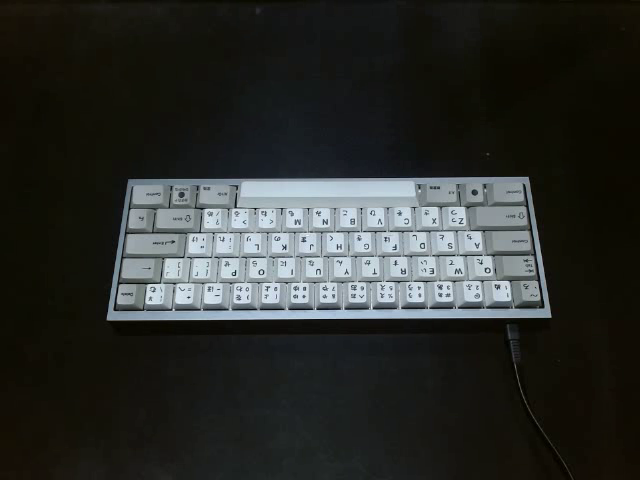
\includegraphics[width=0.7\textwidth]{60.png}
	\caption{A 60\% keyboard in modified \ac{ansi} layout.}
	\label{fig:60}
	\centering
\end{figure}


\section{Significance of the Research}
This research is beneficial for all users of physical keyboards. These include a
majority of the population as there are a lot of professions that rely heavily
on keyboards. Examples include developers, physicians, educators, and
accountants. By having better ergonomics while typing --- by touch typing
correctly --- wrist injuries can be prevented, and typing speed may be
increased.

This research also helps educators, especially early educators teaching beginner
typists. By automatically checking for correct technique, the burden of checking
each student is reduced, and directed interventions for bad habits can be easily
created as students with these bad habits are easily identified.

This research has a direct impact on people that have hand or wrist injuries
that are caused by poor typing habits. By correcting these poor habits, pain
from these injuries will be reduced, and even be prevented from occurring in the
first place. A specific example of this is by reducing ulnar deviation which
affects the nerve that is indicative of \ac{cts} \parencite{toosi2015}.

\chapter{Review of Related Literature}

\section{Keyboard Typing}

Keyboard typing is the process of using a keyboard to input characters in a
system. In the context of this paper, keyboard typing will refer to the act of
using a physical keyboard to input characters into a computer system.

\subsection{Keyboard Layouts and Form Factors}

One key characteristic of a keyboard is its physical attributes. Keyboards come
in a lot of layouts and form factors. Keyboard layouts are the shapes, size, and
positions of a key on a keyboard while the form factor of a keyboard refers to
its shape and dimensions. The form factor also refers to the number of keys included
in the keyboard \parencite{parkkinen2018}. By combining different layouts and
form factors, different permutations of a keyboard can be created.

Different keyboard layouts and form factors also produce different effects for
the user. This is due to how vastly different some keyboard layouts and form
factors are from one another. Some layouts focus on ergonomics, while others
focus on typing speed. Some form factors were designed for aesthetics, while
others focus on comfort and health. As such, different layouts may affect typing
performance, ergonomics, and long-term health effects \parencite{ciobanu2015}.

\subsubsection{ANSI and ISO Layout}

There are two common keyboard layouts around the world --- \ac{iso} and \ac{ansi}.

\citeauthor{ansi} is the standard that first defined the \ac{ansi} layout.
Figure~\ref{fig:ansi} illustrates what the \ac{ansi} layout looks like. This
layout is also used by countries other than America. Examples of countries that
use this layout as its standard are the Philippines, China, and Korea
\parencite{apple-layout}. However, these countries also opt to modify the layout
by adding extra layers to accommodate other character sets.

\citeauthor{iso} is the standard series that defines a framework that is used to
create other layouts. Layouts created from this standard are colloquially called
\ac{iso} Layouts. Countries around the world use this framework to create
layouts that fit the characters in their language. Examples of countries that
use this framework to create their layout are France, Greece, Canada, and Sweden
\parencite{apple-layout}.

Both of these layouts usually utilize the same key ordering. This ordering is
commonly called QWERTY, based on the first five characters of the first row
of this specific layout.

There are other layouts available, however, they are not as common as the two
previously mentioned layouts. Examples of this include \ac{jis}. Other esoteric
layouts, like Tsangan or split-backspace, also exist. These layouts modify the
\ac{iso} and \ac{ansi} standards by adding or removing certain keys to fit the
character set of a language, or for additional keys. Other layouts are also the
same as \ac{ansi} or \ac{iso}, however, these layouts change the arrangement of
the alphabet within the keyboard.

Despite the ubiquity of these common layouts, studies have shown that these
layouts are not ergonomic. The main issue with these layouts is the random
configurations of the letters. The randomness of the layout necessitates
memorization of the layout which reduces the ease of learning, reduces performance
in typing by reducing speed, and increases typing errors
\parencite{ciobanu2015}.

\subsubsection{Keyboard Form Factors}

There is only one common keyboard form factor used worldwide: the full-size
keyboard. This keyboard contains all the keys specified in the keyboard
layout. This includes the alphanumeric keys, the function keys, the navigation
cluster, and the Numpad.

Other common keyboard form factors are based on the full-size keyboard. The name
of these layouts, 60\%, 75\%, and 80\% reference the remaining number of keys
after cutting a portion off from the full-size keyboard. The 60\% keyboards only
contain the alphanumeric cluster while the 80\% and 75\% layouts retain the
navigation cluster and the function keys \parencite{parkkinen2018}. The main
draw for using keyboards with reduced sizes is for aesthetics, space
constraints, and ergonomics.

\begin{figure}[H]
	\centering
	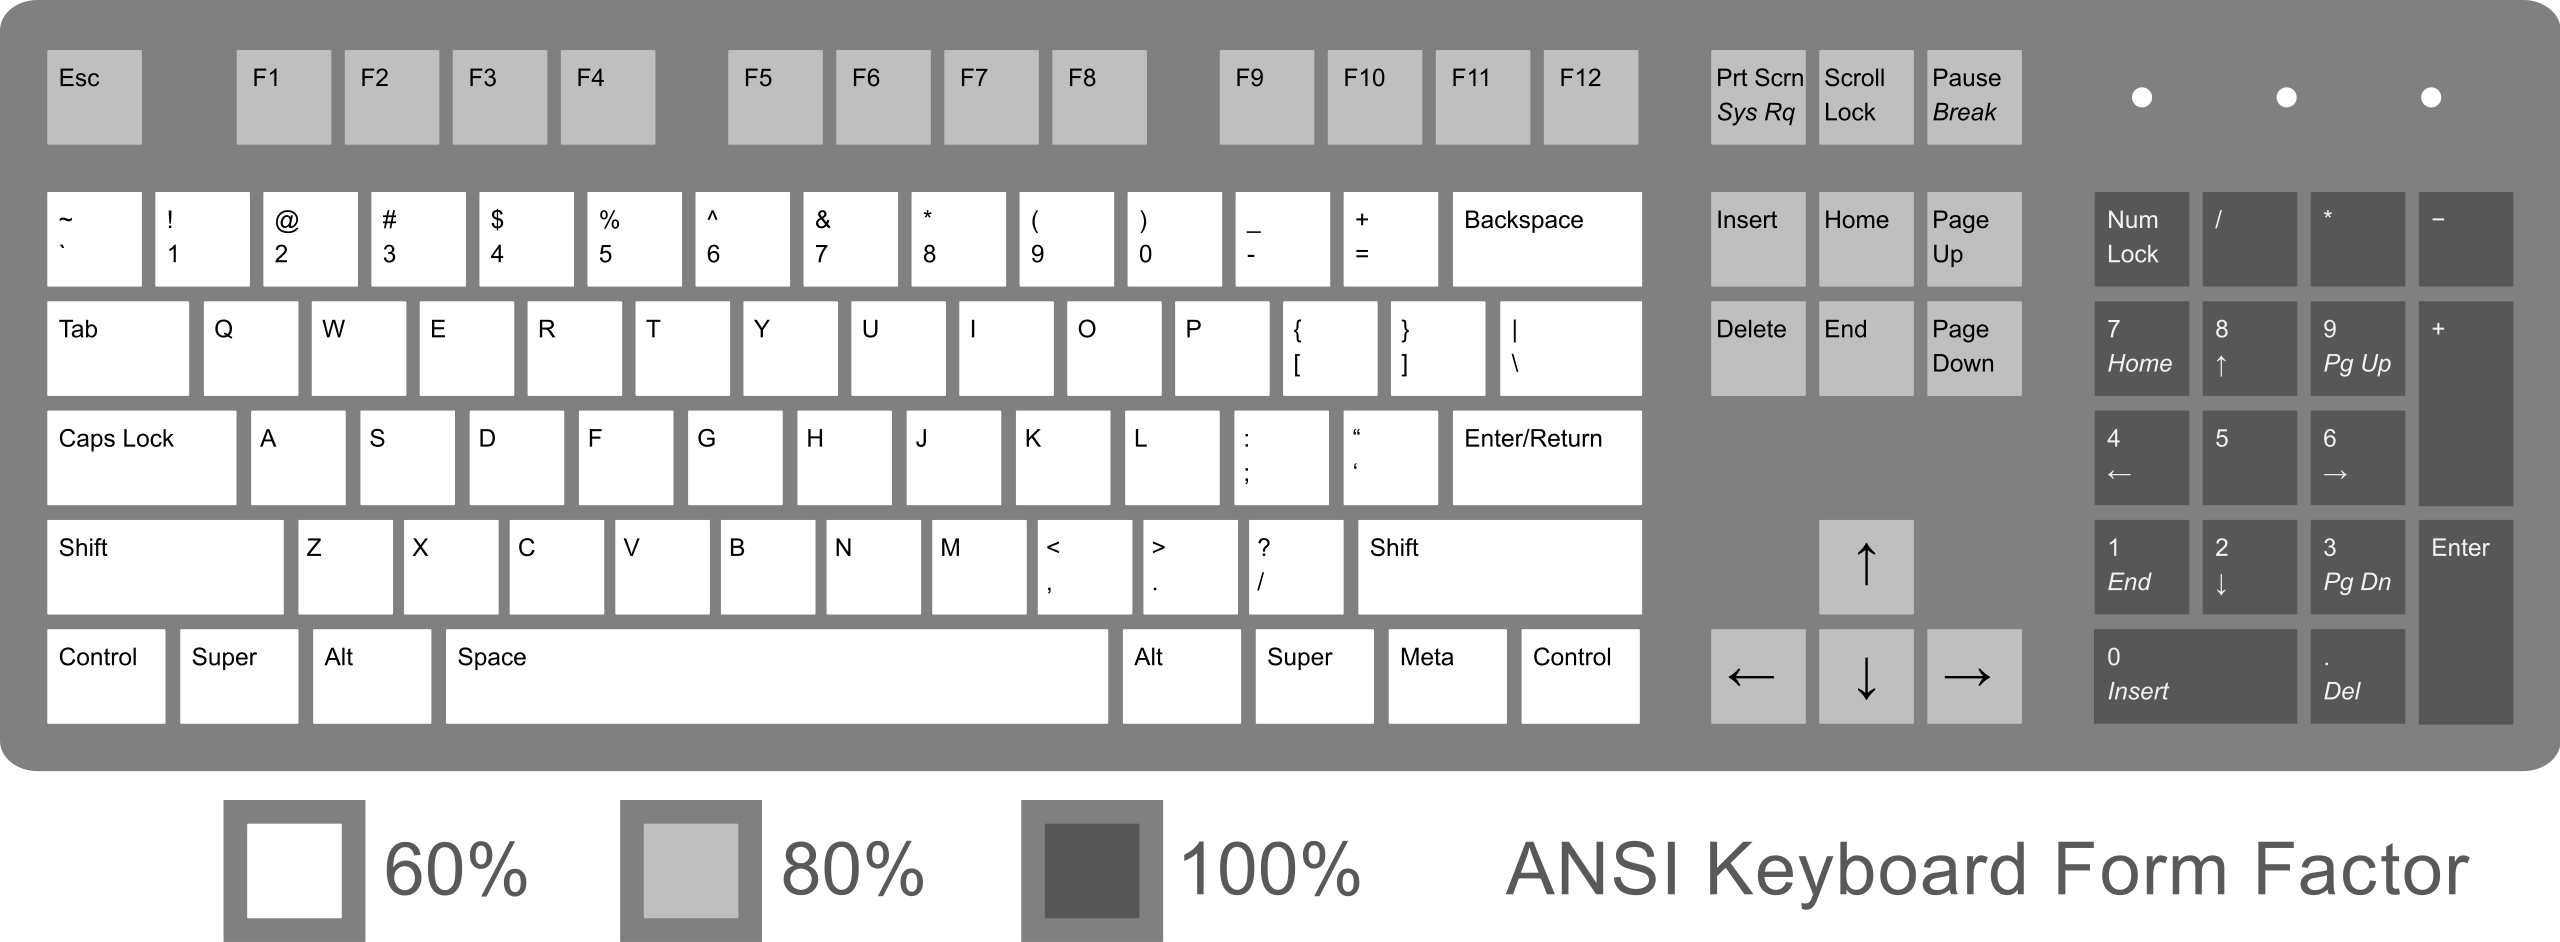
\includegraphics[width=0.8\textwidth]{ansi.png}
	\caption{\ac{ansi} Keyboard layout with form factors. Reprinted from \fullcite{figure-ansi}}
	\label{fig:ansi}
	\centering
\end{figure}

\subsubsection{Ergonomic Keyboards Layouts and Form Factors}

There have been other keyboard layouts and form factors created to mitigate
common issues associated with QWERTY layouts. These include Colemak, Dvorak, and
Alphabetical layouts. However, studies have shown that the layout itself does
not matter as beginners do not necessarily see the keyboard as a structured set,
but rather as a random collection of characters, even if it is alphabetized
\parencite{norman1982},

A different form factor has a great effect on ergonomics. One such example of a
form factor is an ergonomic keyboard developed by Microsoft called Microsoft
Natural MultiMedia Keyboard. \citeauthor{ripat2010} used this keyboard in
determining that ergonomic keyboards can help in reducing symptoms of \ac{neck}.
Figure~\ref{fig:mn} shows the layout of the Microsoft Natural MultiMedia
Keyboard.

\begin{figure}[H]
	\centering
	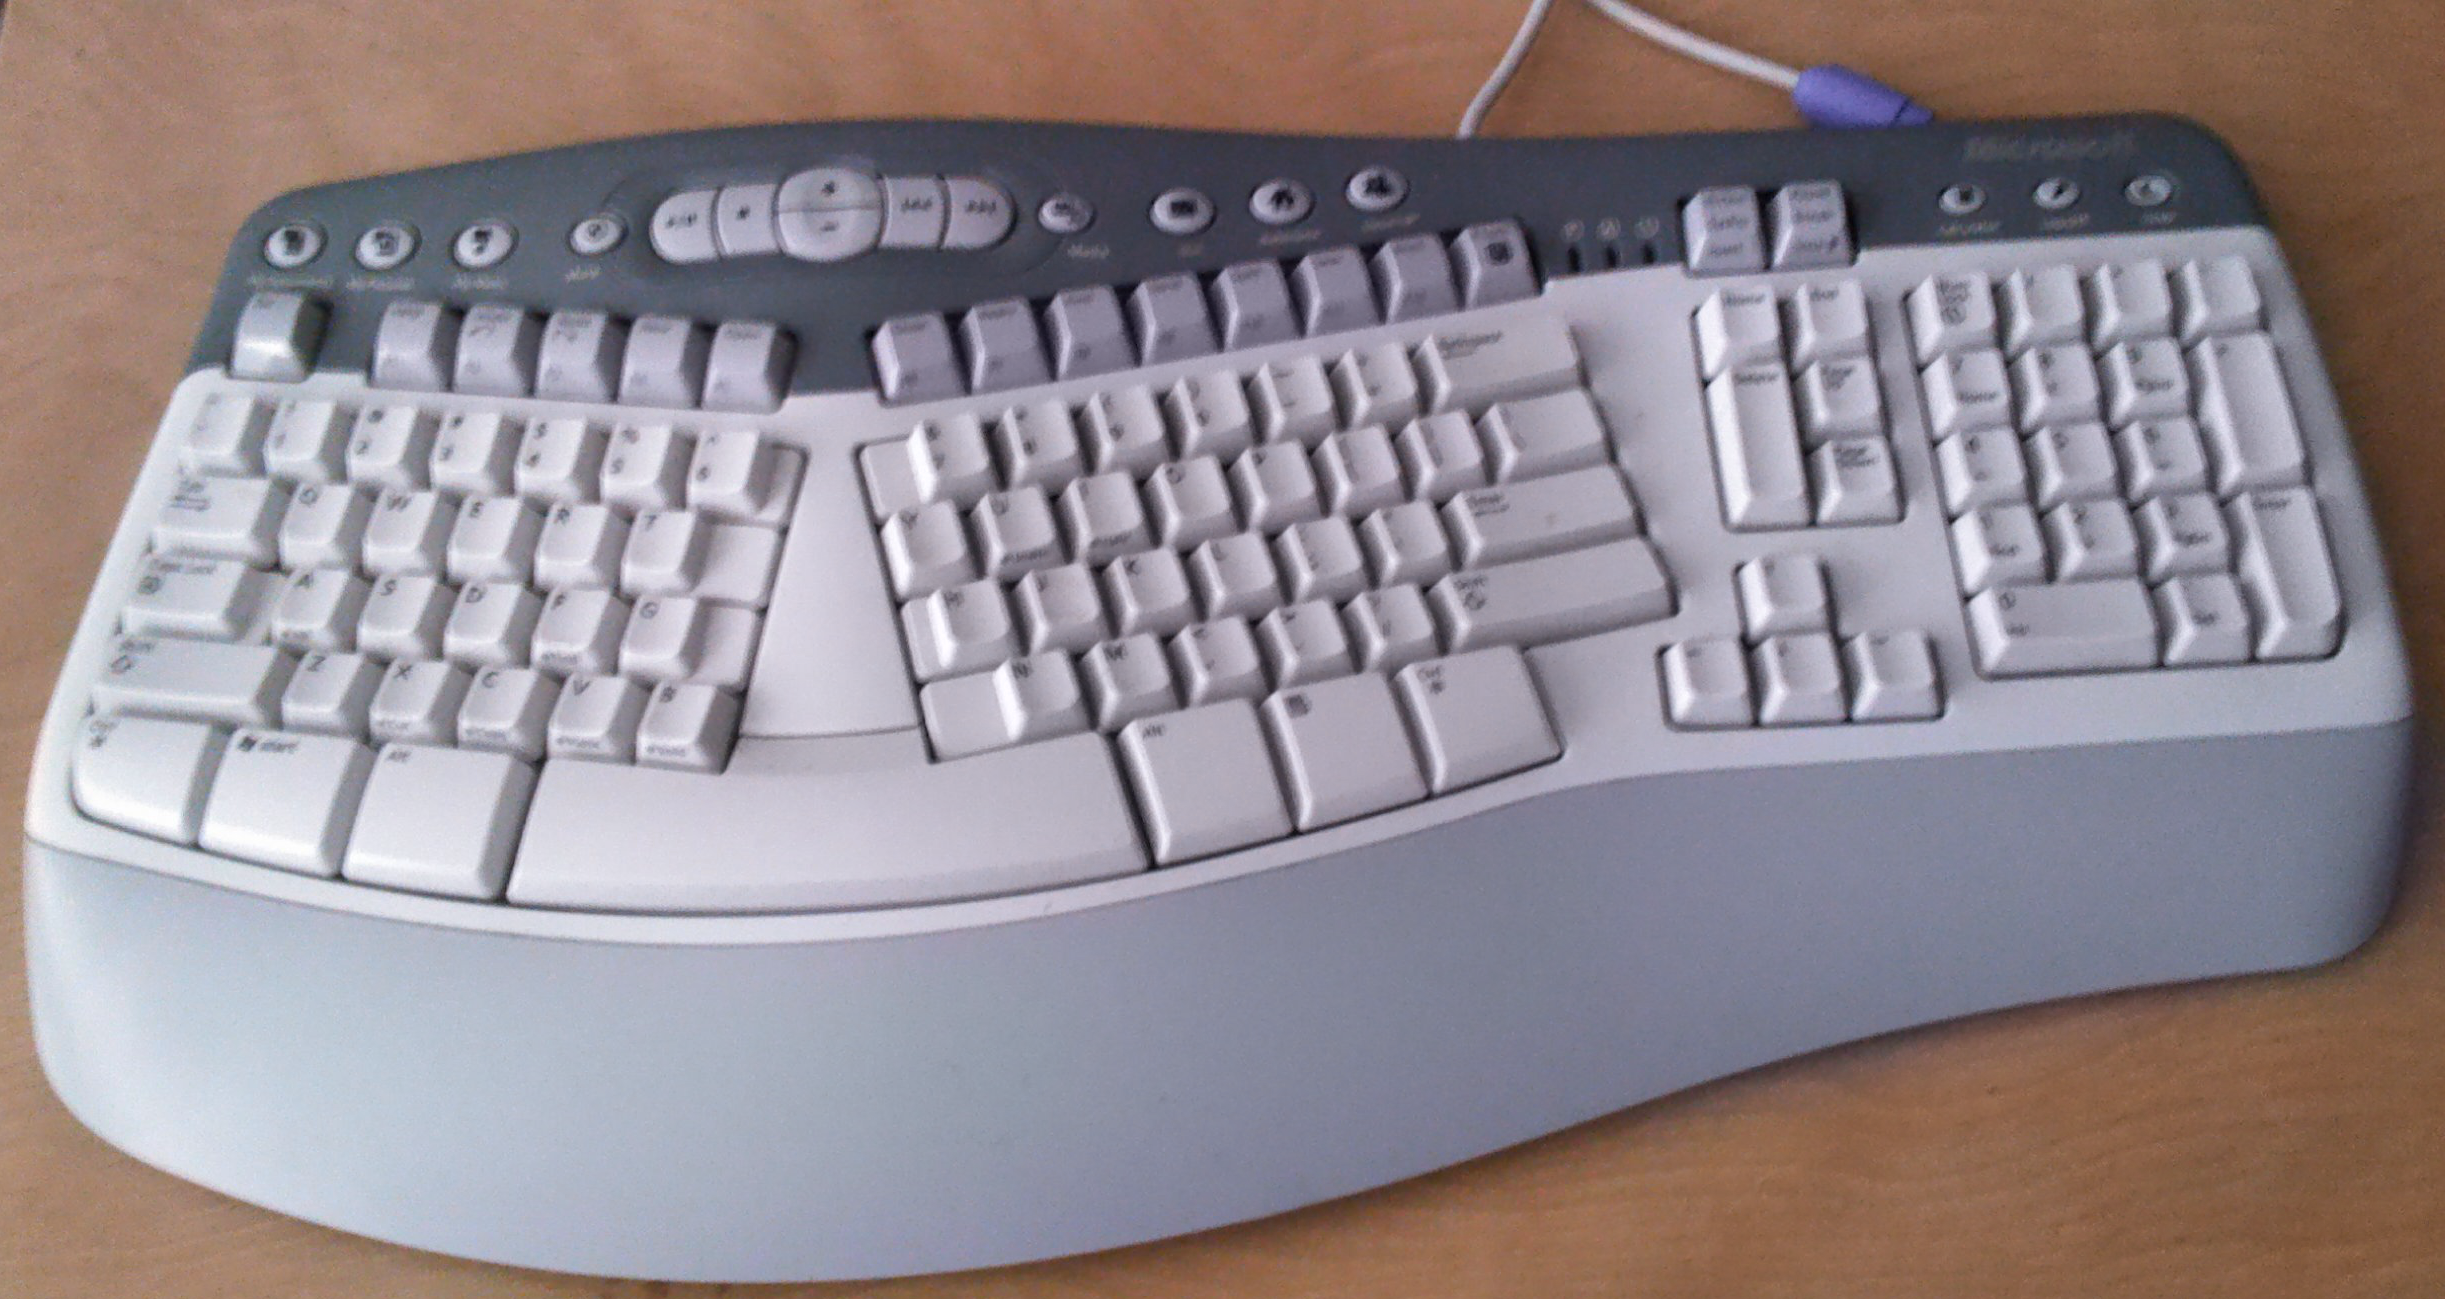
\includegraphics[width=0.8\textwidth]{mn.png}
	\caption{Microsoft Natural MultiMedia Keyboard. Reprinted from \fullcite{mn}}
	\label{fig:mn}
	\centering
\end{figure}

There are other form factors other than the full-size keyboard and variations
thereof that focus on ergonomics. One such example is a split keyboard layout
where the keyboard is split in half, one for the left hand and one for the
right. One such benefit, according to \citeauthor{ergodox}, is a more relaxed
position due to typing at shoulder width.

\subsection{Keyboard Typing Metrics}

There are numerous metrics used to quantify keyboard typing performance. Two
common metrics used in the majority of typing tests include Accuracy and Speed.

\subsubsection{Standardized Keyboard Typing Assessments}

To be able to measure these metrics, a keyboard typing assessment needs to be
done. However, there are no standardized keyboard typing assessments
\parencite{donica2018}. As such, teaching methods and assessments, like
Keyboarding without Tears, Monkeytype, and Keybr, may produce different metrics
for the same typist due to their difference in conducting the assessment.

\subsubsection{Speed}
Speed, also called as entry rate by \citeauthor{arif2009}, measures the number
of characters entered within a specific time frame. The most common metric that
measures speed is \ac{wpm}. \ac{wpm} as defined by \citeauthor{arif2009} is:

\begin{equation}
	WPM = \frac{|T| - 1}{S} \cdot 60 \cdot \frac{1}{5}
	\label{equ:wpm}
\end{equation}
\labelequations{Words per Minute}

Where, $|T|$ is the length of the text, $S$ is the time in seconds spent writing
the text. This time starts directly after the first character has been pressed,
and ends when the last letter has been entered. As such, $1$ is subtracted from
$|T|$, as the time spent to find and press the first character cannot be
accurately determined. However, some typing assessments do not subtract $1$ from
$|T|$. $60$ refers to the number of seconds in a minute and $\frac{1}{5}$
normalizes the metric for the average length of words.


Other metrics also measure speed, but they aren't as commonly used as \ac{wpm}.
These include Characters per Minute, Gestures per Second, Adjusted Words per
Minute, and Keystrokes per Second

\subsubsection{Accuracy}
Accuracy measures the number of correctly pressed characters in an input string.
Accuracy, as defined by \citeauthor{bartnik2021}, is:

\begin{equation}
	ACC = \frac{|C|}{|T|} \cdot 100\%
\end{equation}
\labelequations{Accuracy}

Where $|C|$ is the number of correct characters and $|T|$ is the length of the
text.

The inverse of accuracy is error rate, where the number of incorrectly pressed
characters is measured instead. \citeauthor{arif2009} describe 5 common error
rate metrics: Error Rate, Minimum String Distance Error Rate, Keystroke per
Character, Erroneous Keystroke Error Rate, and Total Error Rate.

\subsubsection{Limitations of the Metrics}
These metrics are all based on the inputted characters by the user. These
metrics do not take into account other aspects of keyboard typing such as
posture, hand and wrist positions, and finger placement. Consequently, these
metrics do not give a full picture of the performance of the person typing, and
they only provide a cursory view of how a person types.

\subsection{Keyboard Typing Methodology}
Keyboard typing can be accomplished in numerous ways. The main difference
between the different methodologies is the number of fingers used when typing
and how the typist navigates the keyboard to find the keys. The methodology
ranges from Hunt and Peck to Touch Typing, with variations of the two in
between.

Hunt and Peck uses one finger on one hand to press a key. This method is aided
by using vision to locate the specific key to press \parencite{hoot1986}. On the
other hand, Touch typing uses standard QWERTY mapping to type without using
visual cues. \parencite{dobson2009touch} This mapping involves assigning certain
fingers to certain keys. Figure~\ref{fig:touch-type} is the standard QWERTY
mapping used for an \ac{ansi} layout. Kinesthesis and proprioception are used in
locating the keys \parencite{logan2016}.

\begin{figure}[H]
	\centering
	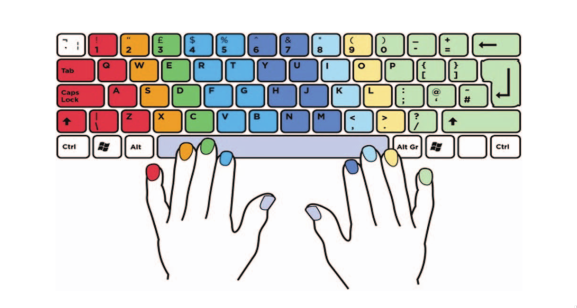
\includegraphics[width=0.8\textwidth]{touch-type.png}
	\caption{Standard QWERTY mapping for \ac{ansi}. Reprinted from \fullcite{logan2016}}
	\label{fig:touch-type}
	\centering
\end{figure}

\subsection{Typing Speed Statistics}

Median typing speed using a keyboard with QWERTY layout, based on test data from
\textcite{keybr}, is $\approx37.5$ \ac{wpm}. This median is taken from all the test
results they have gathered from all of their users.

\textcite{monkey-stats} released a dataset showing the speed of 12678 members of the
Monkeytype community with the speed role. The dataset shows the fastest time
that these members have achieved on 60-second tests. The median of the dataset
lies in the 100--109 \ac{wpm} range, with 52.74\% of the community having top
speeds slower than 100 \ac{wpm}.

\textcite{arif2009} also performed a survey with 12 participants using
multiple typing methods. They got an average \ac{wpm} of 75.85 with a standard
deviation of 15.61 when their participants used a physical QWERTY layout. This
average \ac{wpm} was also the highest among the other typing methods the
researchers studied.

\section{Keyboard Typing in Education}

Today, students are expected to type essays, articles, and other submissions
using word processors \parencite{poole2016}. Testing is also commonly done using
computerized assessments which require the need for keyboards
\parencite{moodle}. As such, there is a need for students to be well versed in
keyboard typing and for keyboard typing to be part of the curriculum.

Keyboard typing has been a part of this curriculum for a long time, with studies
about effective methods to teach keyboard typing reaching as far back as 1986
\parencite{hoot1986}. Studies have continued to this day to continue to optimize
and improve methods of teaching keyboard typing to students.

These studies start teaching kids at the kindergarten level and the studies try
to optimize the teaching methods to improve the speed and accuracy of typing of
the learners.

\subsection{Expectations of Keyboard Proficiency}

In the United States, keyboard typing is an expected learning outcome for third
grade in the Common Core State Standards \parencite{ccs}. At this grade level,
only basic keyboard typing skills are required. By fourth grade, students are
expected to have enough proficiency to type one page in one sitting. This is
increased to two pages by fifth grade.

In the Philippine context, the \citeauthor{deped} expects learners with a mental
age of 4--6.9 years old to use correct posture and locate characters, learners
with a mental age of 7--11.9 are introduced to home row finger placement, and
learners with a mental age of 12 and above are expected to ``use proper typing
technique with efficiency and accuracy without looking at the keyboard''
\parencite{deped}.

\subsection{Current Teaching Methods}

Current teaching methods involve replicating a given text. Learners then copy
the text into a given text field that records the typed characters. Correct and
incorrect characters are then identified, and suitable errors are presented.
Afterward, metrics, such as \ac{wpm}, and accuracy are given
\parencite{bartnik2021, typeracer}.

Through this process, the learner goes through the three stages of Motor
Learning Theory. The student undergoes the cognitive stage where they try to
understand and create strategies to accomplish the given task. Then the
associative stage follows where the strategies and skills learned from the
previous stage are refined. At this stage, the learners are expected to rely less
on visuals to locate the keys and more on kinesthesis. In the final stage, the
autonomous stage, the learner does not rely on visuals at all and focuses on
using kinesthetic feedback to find the keys. By this point, the learner has
progressed from using Hunt and Peck, to becoming proficient in touch typing.
\parencite{donica2018}

\subsubsection{Keyboarding without Tears}

Keyboarding without Tears is a web-based application and curriculum that teaches
students touch typing. However, one key differentiator of this curriculum is the
usage of a row-based standard mapping, rather than a column-based standard
mapping that is common in other teaching guides. Figure~\ref{fig:kwt} shows the
standard mapping used in this curriculum.

This curriculum is self-directed and learners can learn at their own pace. At
its core, the curriculum is designed to be 36-week long with 5--10 minutes of
lessons per day. The lessons in the curriculum follow the three stages of
Motor Learning Theory \parencite{kwt}.

\begin{figure}[H]
	\centering
	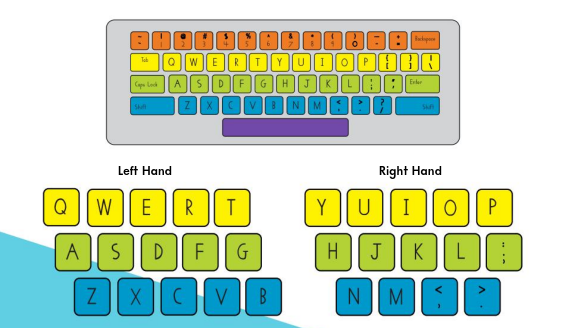
\includegraphics[width=0.8\textwidth]{kwt.png}
	\caption{Row based standard mapping. Reprinted from \fullcite{kwt}}
	\label{fig:kwt}
	\centering
\end{figure}


\subsubsection{Monkeytype, Typeracer}

These two keyboard typing tests are similar. They follow a common experience
where users type a predetermined phrase, quote, or random words, and metrics are
given after the test. Afterward, the learners may try the test again, or choose
another set of words to type. These typing tests do not have a structured
curriculum for learning how to touch type. It is left to the learner to practice
and learn on their own \parencite{bartnik2021, typeracer}.

\subsubsection{Keybr}

Keybr is similar to Monkeytype and Typerace, in that they also have the users
type a predetermined phrase, quote, or random words. However, this application
has more guidance compared to the two. Keybr uses statistics to create typing
lessons that are appropriate to the current typing proficiency of the learner.
The words selected are random at first, and the skill level of the learner is
determined by the performance of the user with these words and characters. The
information gathered is then used to generate new words for the next iteration.
As an example, if a learner has difficulty typing the letter q, the next
iterations will have a lot of words that contain the letter q.

Statistics from their website show that this learning method is successful, with
some learners improving their typing speed by 20--40 \ac{wpm} \parencite{keybr}.

\section{Keyboard Typing in Health}

There have been a lot of studies that show the effect of keyboard typing, and
its associated movements (or lack thereof), affects the human body. These
studies have shown that keyboard typing affects our neck, shoulder,
upper limb, wrist, arms, and fingers \parencite{szeto2005, baker2007digit}

\subsection{Health Issues arising from Keyboard Typing}

\ac{neck} are a common issue that is associated with an elongated length of time
maintaining a static posture. When using the computer, the posture commonly
adapted by users has the neck and shoulder regions in a static hold for a long
time. This results in forward neck flexion and increased muscle tension
\parencite{szeto2005}.

In addition, it has been shown that 22\% of computer users sustain
musculoskeletal disorders of the upper extremity. This includes the neck,
shoulder, hands, and wrists. \parencite{gerr2002}

Carpal tunnel syndrome is also a common issue in the general population. This is
caused by the chronic compression of the median nerve. There is a common belief
that typing is one main cause for the disorder \parencite{carpal-myth}. There
are no definite conclusions if this myth is true, however, a study by
\citeauthor{toosi2015} found that typing causes ulnar deviation, especially if
done without proper form. This ulnar deviation contributes to the swelling of
the median nerve during and after typing. However, the authors noted that it is
unclear if this swelling leads to long-term nerve injury.

\subsection{Finger and Wrist Kinematics}
The way people move their hands, wrists, and fingers differs between each
person. This can be attributed to the different typing styles each person has.
One key difference between people is the angle of the fifth digit.

However, there are some common movements and positions regardless of typing
style: flexion, or the curving of the fingers, across the fingers, is decreasing
across the hand, with the 2nd digit having the least flexion. This may be due to
the instinct to reduce pronation of the hand, which in turn increases the
distance of the 2nd digit to the keyboard. In addition, some people isolate or
extend one of their thumbs, usually the one not used for pressing a key. This is
also true for some people that do not use their fifth digit during typing
\parencite{baker2007}.

The movement and angle of the wrists also depend on the typing style of the
typists. Some people do not reposition their hands, while others do. This
difference comes from the way these people reach for certain far-away keys. Some
stretch their fingers to reach far-away keys, while others move their entire
hand to reach these keys.

For those that reach their keys by stretching their fingers, there is an
increased probability that the wrists and fingers adapt to non-neutral postures.
These include wrist extension, ulnar deviation, and pronation, which may cause
musculoskeletal disorders of the upper extremity (\textcite{marklin1999} as cited in
~\textcite{baker2007})

\section{Finger and Hand Tracking}
Finger and Hand tracking is a method of tracking fingers and hands in 3D space
using motion capture systems or computer vision. This technique allows computers
to perform actions and analyzes the motions and positions of these body parts.


\subsection{Types of Tracking}

\subsubsection{Hardware Aided Solutions}

Motion Capture Systems allow for capturing detailed skeletal motion in humans.
These systems usually capture full-body motion, focusing on large parts of the
human body, such as the torso, limbs, and head.

However, motion capture systems have difficulty in tracking more articulated
body parts --- with the fingers being one of them. The industry standard for
capturing finger movements is through the use of an optical marker-based motion
capture system. This is due to its ability to capture natural motion accurately.

This method uses cameras to triangulate the 3D location of markers attached to
the limbs of a person. For finger tracking, 13--20 markers are placed on the
fingers, and cameras are brought closer to track the small movements of the
finger \parencite{wheatland2015}.

But this method is cost-prohibitive, and cannot handle occlusions well.
\citeauthor{alexanderson2016} present a method for an optical marker-based
motion capture system that can predictably recover from self-occlusion and has a
better performance compared to previously used algorithms, however, the issue of
cost and self-occlusion persists.

Bend-sensor gloves are also an option for finger tracking. These gloves have
sensors within them that track joint angles in the hand and fingers. One key
differentiator of this solution compared to the others is the removal of
self-occlusion in the data. As such, this is commonly used in sign language, and
gesture recognition due to its accuracy.

However, these gloves need a lot of time to calibrate as cross-coupling of the
sensors proves a problem. Cross-coupling is prevalent because the movement of
one finger also moves other parts of the hand. These movements may cause a
sensor aimed to track a specific movement of a different part of the hand to
inadvertently detect a movement when there should be none
\parencite{wheatland2015}.

\subsubsection{Computer Vision}

At its core, Computer Vision aims to perform tasks that the human visual system
can do \parencite{cern}. This includes object classification, tracking, gesture
recognition, and face recognition. At the present, most computer vision systems
utilize deep learning algorithms, and convolutional networks to gather
information from an image, or a set of images. One such example of a
convolutional network used in computer vision is Inception by
\citeauthor{szegedy2015} which proposes a convolutional neural network
architecture for object classification and detection.

\subsection{Available CV Solutions for Tracking}

\subsubsection{OpenCV}

OpenCV is an open-source library that provides ${\approx2500}$ optimized
algorithms for computer vision and machine learning. This library is widely used
by companies, researchers, and open source communities that utilize computer
vision and machine learning in their projects. Examples of companies that use
OpenCV include Google, Sony, and Honda.

The library has C++, Python, Java, and Matlab interfaces. The library also supports
Windows, Linux, Android, and macOS, allowing for great developer experience, and
wide deployment capabilities \parencite{opencv}.

\subsubsection{MediaPipe}
\label{section:rrl-mediapipe}

MediaPipe is an open-source computer vision framework that allows developers to
create a perception pipeline. This perception pipeline is a directed graph of
calculators. Data passes through the graph as packets and a group of packets
constitutes a data stream. As the data passes through the pipeline, the
calculators, produce the desired output.

This framework allows for performant object detection, hand and finger tracking,
and human pose detection. The framework also allows for combining multiple
features, by adding them to the graph as calculators. MediaPipe has C++, Python,
JS, and Coral interfaces. It also supports Android and iOS devices
\parencite{mediapipe}.

Examples of projects that utilized MediaPipe and its solutions include a
real-time hand gesture recognition system by \textcite{mediapipe-sample-1} which
utilized MediaPipe Hands. Another example is by \textcite{mediapipe-sample-2}
who utilized MediaPipe Hands to track movements during pen spinning
competitions. \textcite{mediapipe-sample-3} developed a real-time sign language
recognition program using MediaPipe Hands.


\subsubsection{MATLAB}
MATLAB is a programming platform for the analysis and designing of systems.
MATLAB is commonly used by engineers and scientists for computational
mathematics \parencite{what-matlab}.

A toolbox offered by MATLAB is the Computer Vision Toolbox which contains
algorithms, and functions for use in the development of computer vision, 3D
vision, and video processing systems. By using the available algorithms in the
toolbox, such as YOLOv2, and ACF, hand detection and gesture recognition are
made possible in the platform \parencite{matlab}.

\subsection{Applications}

There have been multiple applications and products that utilize hand and finger
tracking as their main component.

\textcite{dorf2001} present a use case for finger tracking in augmented
environments. In the paper, interaction in a virtual environment through the use
of gestures. The tracking system uses an optical marker-based motion capture
system where the user wears a glove with retroreflective markers.

\textcite{chiang2014} used a Kinect, a 3D sensing device by Microsoft that
uses depth data, to track fingers to play virtual instruments. Virtual Pianos
and Guitars were created and played with reliable and stable tracking.

\textcite{yousaf2014} created a virtual keyboard that operates using finger
tracking. The tracking uses the movement of the finger joints as the basis for
selecting which key to press. The tracking first detects where the hands are.
The result of the detection is then piped to a different algorithm for finger
joint localization. These are then used to generate finger joint trajectories
using kernel tracking. A Dynamic Bayesian Network then uses feature vectors from
these trajectories to classify, detect, and recognize keystrokes.

\section{Summary of the Research Gap}
While there are a lot of applications and curricula aimed at teaching touch
typing, there is no automated system available that detects if a person uses the
correct finger to press a key.

By having this system, educators can accurately determine if and when a student
is having a hard time typing and if these students will need an intervention to
correct mistakes.

This is also important because certain movements and hand positions will cause
nerve and muscular disorders that will impact the user. By correcting these
problematic movements and hand positions, these disorders can be prevented.

\chapter{Methodology}

This section provides an overview of the development and testing of a real-time
finger-key identification module. First, the experimental setup used for data
collection will be presented. Following that, the algorithm used to implement
real-time finger-key identification will be discussed. The process of training
and testing the developed algorithm comes next. Afterward, the development and
design of the proof of concept trainer will be described. Finally, this section
introduces two metrics that were developed to quantify correct finger placement
during typing tests.

\section{Setup}
\label{section:metho-setup}

The experimental setup and configuration were composed of three elements: the
camera, the keyboard, and the environment. This setup was used to collect data
points to measure the algorithm's ability to perform finger-key identification
in a controlled environment. Figure~\ref{fig:metho-setup} is an image of the
experimental setup.


\begin{figure}[H]
	\centering
	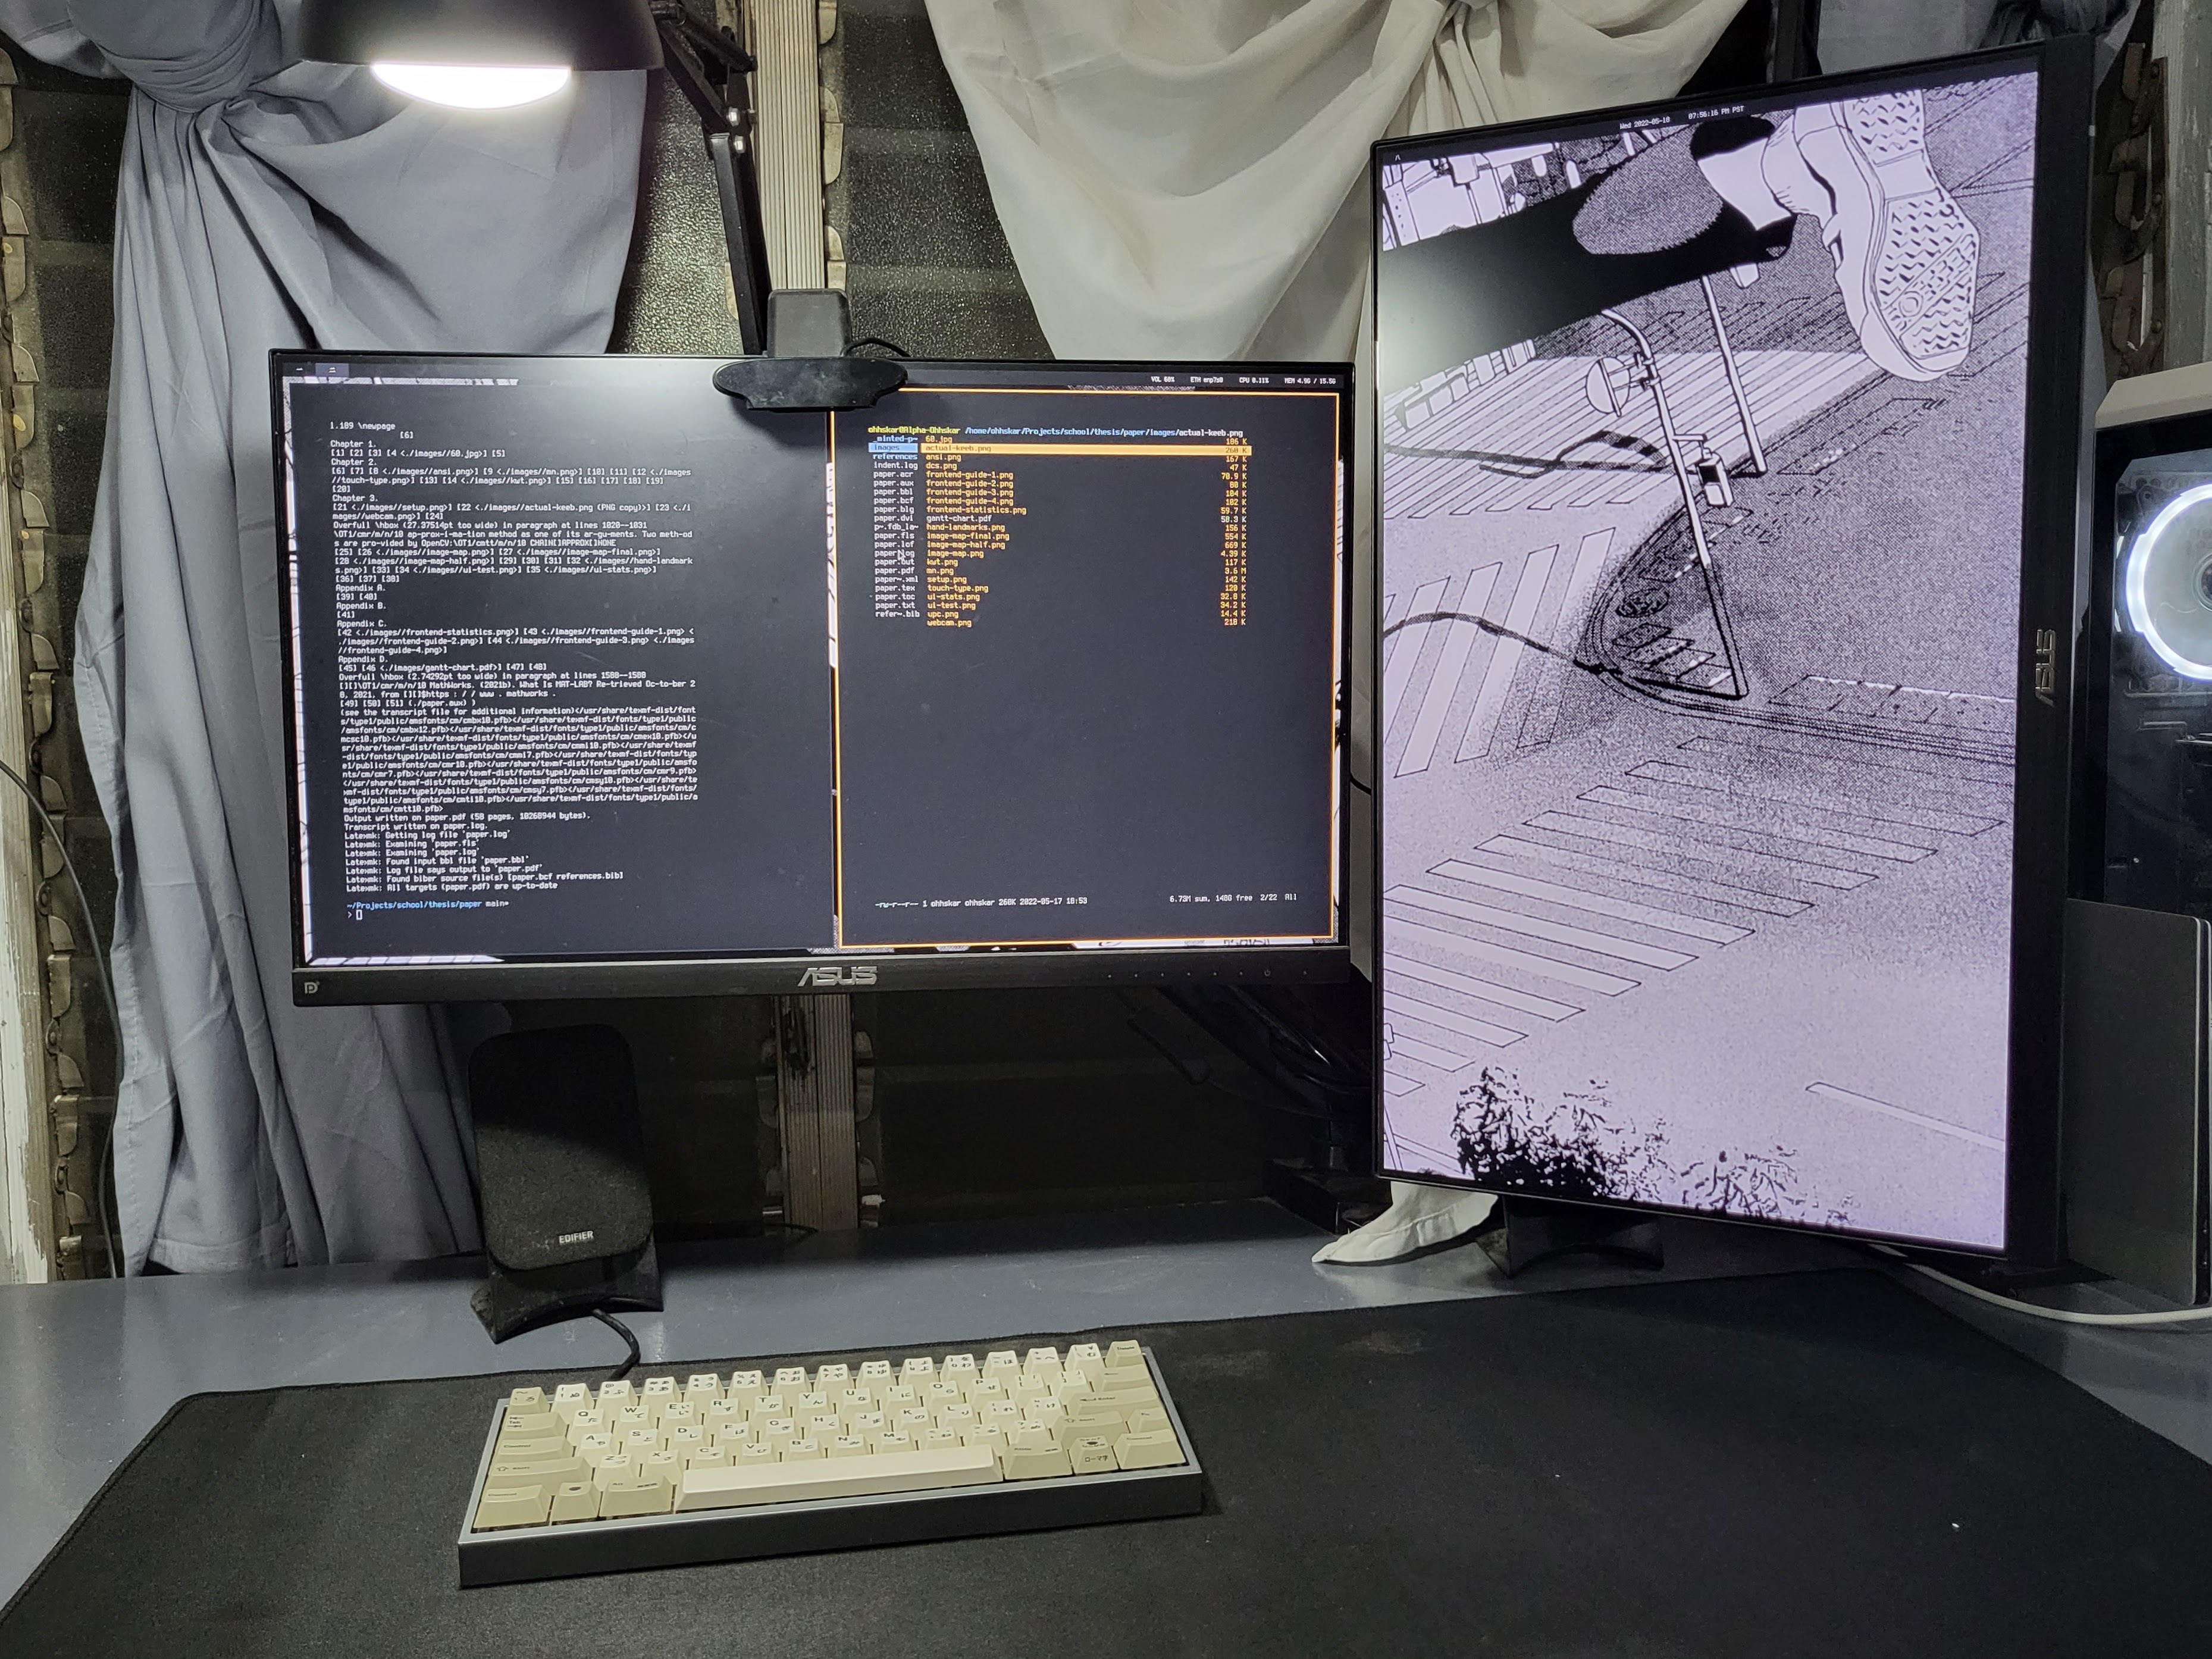
\includegraphics[width=0.8\textwidth]{full-setup.jpg}
	\caption{The experimental setup}
	\label{fig:metho-setup}
	\centering
\end{figure}

\subsection{Camera}
The setup used a single monocular camera positioned in a top-down view. The
camera captures the entirety of the keyboard and the movement of the ten
fingers. To do so, it was mounted on top of the monitor with the camera pointed
down towards the table. Figure~\ref{fig:metho-setup-camera-placement}
illustrates how the camera was mounted over the monitor and
Figure~\ref{fig:metho-setup-keeb} is a picture taken with the camera at this
position.

\begin{figure}[H]
	\centering
	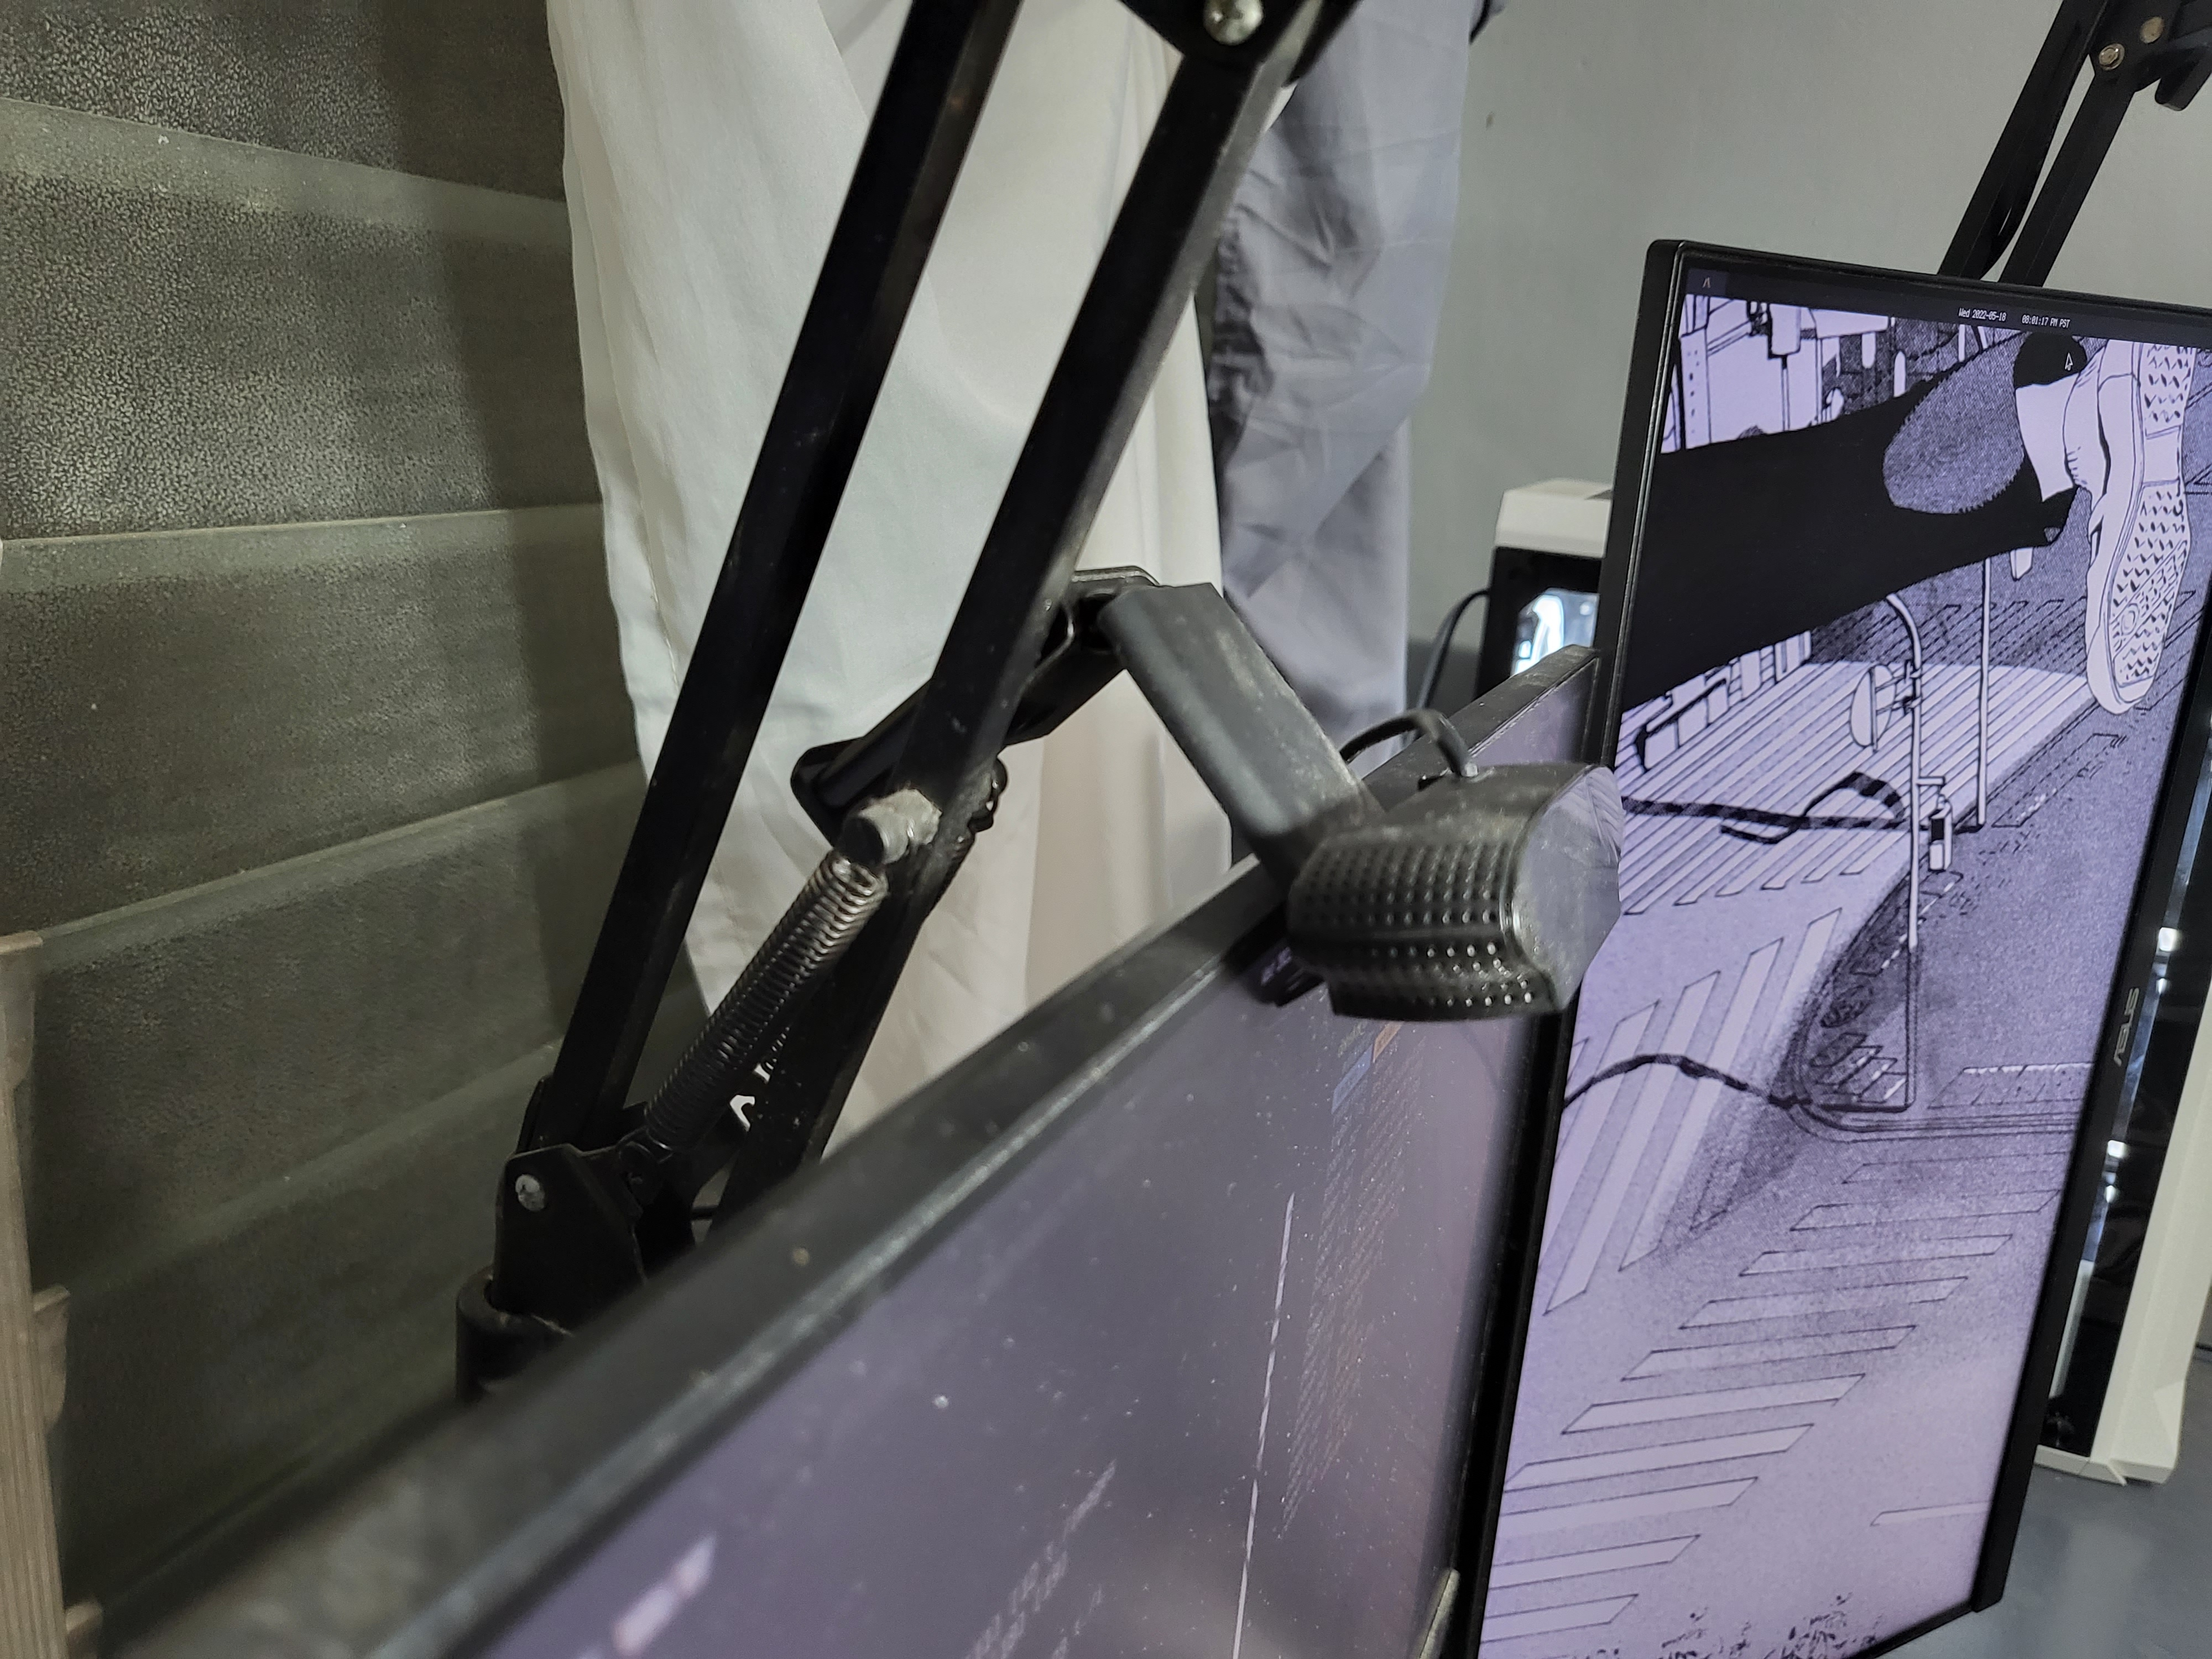
\includegraphics[width=0.8\textwidth]{camera-placement.jpg}
	\caption{The camera angled downwards to capture the keyboard}
	\label{fig:metho-setup-camera-placement}
\end{figure}

\begin{figure}[H]
	\centering
	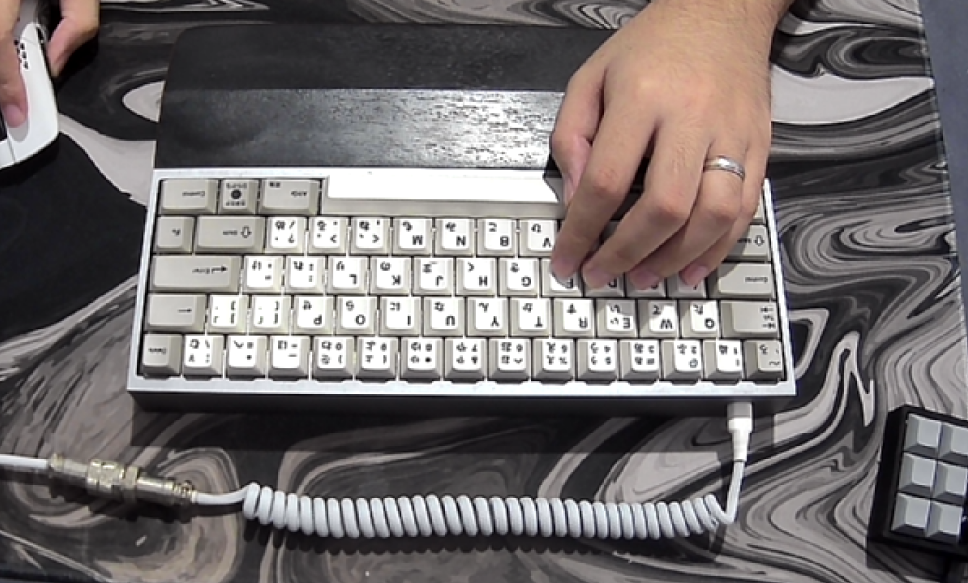
\includegraphics[width=0.8\textwidth]{actual-keeb.png}
	\caption{Image captured by the camera in one of the training iterations}
	\label{fig:metho-setup-keeb}
\end{figure}

The specific camera used was a Logitech C920. It is a 3 megapixel webcam that
is capable of capturing color video in 1080p/30fps and 720p/30fps with a
diagonal field of view of 78\degree. For the setup, the camera captured the
video in 480p/30fps. This camera has a universal mounting clip that allows the
camera to be correctly positioned within the experimental setup
\parencite{logitech}.

\subsection{Keyboard}
\label{section:metho-keeb}

The keyboard used was a 60\% keyboard as shown in
Figure~\ref{fig:metho-setup-keeb}. This limited the necessary mapping for the
algorithm to the alphanumeric portion of the keyboard. This keyboard choice also
reduced the area that the camera captured, as this keyboard type is considerably
smaller compared to a full-size keyboard. The keyboard also had its keycaps and
case in a light color that contrasted the dark surface it was placed on. It also
had a dark USB-C cable to blend with the dark surface. These color coordination
steps improved initial keyboard detection.

In addition, the keyboard layout was a modified \ac{ansi} layout. The majority
of the keys remained the same, however some keys were changed: the pipe key was
replaced by the backspace key, the backspace key was replaced by the pipe key
and a delete key, and the bottom row has a longer spacebar. Overall, these are
minor changes that does not affect the alphanumeric keys that are predominantly
used in typing.

\subsection{Computer}
The computer used to run the algorithm is a desktop computer. The specifications
of this computer is shown in Table~\ref{tab:table-specs}.

\begin{table}[H]
	\small
	\centering
	\caption{\label{tab:table-specs}Computer Specifications}
	\begin{tabular}{ p{0.3\textwidth} p{0.6\textwidth} }
		\toprule
		Component & Specification                          \\
		\midrule
		CPU       & AMD Ryzen 5 3600                       \\
		GPU       & AMD Radeon RX 5600 XT                  \\
		RAM       & G.Skill Trident Z Neo RGB 16GB 3200mhz \\
		Storage   & Samsung SSD 850 EVO                    \\
		OS        & Arch Linux                             \\
		\bottomrule
	\end{tabular}
\end{table}

\subsection{Environment}
The setup was lit with a lamp besides the camera. This light source evenly lit
the keyboard and the fingers used for typing. The light source used was a common
LED bulb rated at 9 watts with 700 lumens. This light is white with a color
temperature of 6500k.

In addition, the surface where the keyboard was placed was solid black
without any variation of color. This also improved initial keyboard detection.

\section{Algorithm}
\label{section:metho-algo}

\subsection{Computer Vision based Keyboard Detection, and Key Mapping}
\label{section:metho-algo-keyboard}

A computer vision algorithm was created as a starting point for mapping the keys
of the keyboard within a video. A rough flowchart of the algorithm is shown in
Figure~\ref{fig:metho-algo-key-flow}.

\begin{figure}[H]
	\centering
	\begin{tikzpicture}[font=\small,thick]
		\node[draw,
			rounded rectangle,
			minimum width = 2.5cm,
			minimum height = 1cm,
			inner sep = 3mm
		] (start) {START};

		\node[draw,
			trapezium,
			trapezium left angle = 65,
			trapezium right angle = 115,
			trapezium stretches,
			below=of start,
			minimum width=3.5cm,
			minimum height=1cm,
			inner sep = 3mm
		] (input) {Input Frame};

		\node[draw,
			below=of input,
			minimum width=3.5cm,
			minimum height=1cm,
			inner sep = 3mm
		] (map) {Get Image Map};

		\node[draw,
			below=of map,
			minimum width=3.5cm,
			minimum height=1cm,
			inner sep = 3mm
		] (contours) {Get Key Contour Points};

		\node[draw,
			trapezium,
			trapezium left angle = 65,
			trapezium right angle = 115,
			trapezium stretches,
			below=of contours,
			minimum width=3.5cm,
			minimum height=1cm,
			inner sep = 3mm
		] (output) {Key-Edge Coordinates Map};

		\node[draw,
			below=of output,
			rounded rectangle,
			minimum width=2.5cm,
			minimum height=1cm,
			inner sep = 3mm
		] (end) {END};

		\draw[-latex] (start) edge (input)
		(input) edge (map)
		(map) edge (contours)
		(contours) edge (output)
		(output) edge (end);

	\end{tikzpicture}
	\caption{Flowchart of Keyboard Detection and Mapping Algorithm}
	\label{fig:metho-algo-key-flow}
\end{figure}

\newpage

\subsubsection{Get Image Map}
The first portion of the algorithm creates an image map that is overlaid over
the detected edges of the keyboard. The flowchart for this function is shown in
Figure~\ref{fig:metho-algo-key-image-map}.

\begin{figure}[H]
	\centering
	\begin{tikzpicture}[font=\small,thick]
		\node[draw,
			rounded rectangle,
			minimum width = 2.5cm,
			minimum height = 1cm,
			inner sep = 3mm
		] (start) {START};

		\node[draw,
			trapezium,
			trapezium left angle = 65,
			trapezium right angle = 115,
			trapezium stretches,
			below=of start,
			minimum width=3.5cm,
			minimum height=1cm,
			inner sep = 3mm
		] (input) {Input Frame};

		\node[draw,
			below=of input,
			minimum width=3.5cm,
			minimum height=1cm,
			inner sep = 3mm
		] (gray) {Convert to Grayscale};

		\node[draw,
			below=of gray,
			minimum width=3.5cm,
			minimum height=1cm,
			inner sep = 3mm
		] (denoise) {Denoising};

		\node[draw,
			below=of denoise,
			minimum width=3.5cm,
			minimum height=1cm,
			inner sep = 3mm
		] (edge) {Edge Detection};

		\node[draw,
			below=of edge,
			minimum width=3.5cm,
			minimum height=1cm,
			inner sep = 3mm
		] (thresh) {Thresholding};

		\node[draw,
			right=of gray,
			minimum width=3.5cm,
			minimum height=1cm,
			inner sep = 3mm
		] (contours) {Find Contours};

		\node[draw,
			below=of contours,
			minimum width=3.5cm,
			minimum height=1cm,
			inner sep = 3mm
		] (sort) {Simplify Contour};

		\node[draw,
			below=of sort,
			minimum width=3.5cm,
			minimum height=1cm,
			inner sep = 3mm
		] (transform) {Transform Image Map};

		\node[draw,
			trapezium,
			trapezium left angle = 65,
			trapezium right angle = 115,
			trapezium stretches,
			below=of transform,
			minimum width=3.5cm,
			minimum height=1cm,
			inner sep = 3mm
		] (output) {Virtual Image Map};

		\node[draw,
			below=of output,
			rounded rectangle,
			minimum width=2.5cm,
			minimum height=1cm,
			inner sep = 3mm
		] (end) {END};

		\node[coordinate, right = 0.5cm of thresh] (below) {};
		\node[coordinate, right = 0.5cm of gray] (top) {};

		\draw[-latex] (start) edge (input)
		(input) edge (gray)
		(gray) edge (denoise)
		(denoise) edge (edge)
		(edge) edge (thresh)
		(thresh) -- (below) |- (top) |- (contours)
		(contours) edge (sort)
		(sort) edge (transform)
		(transform) edge (output)
		(output) edge (end);

	\end{tikzpicture}
	\caption{Flowchart of Get Image Map}
	\label{fig:metho-algo-key-image-map}
\end{figure}

\newpage

\paragraph{Convert to Grayscale}
The input frame from the camera was converted to a 256 level grayscale image
using \texttt{cvtColor} of OpenCV \parencite{opencv-cvtColor}. This step was
performed because future steps of the algorithm did not require color values to
work. In addition, this step optimized the algorithm as the number of dimensions
analyzed was reduced. Figure~\ref{fig:metho-algo-convert} is the output of this
step.

\begin{figure}[H]
	\centering
	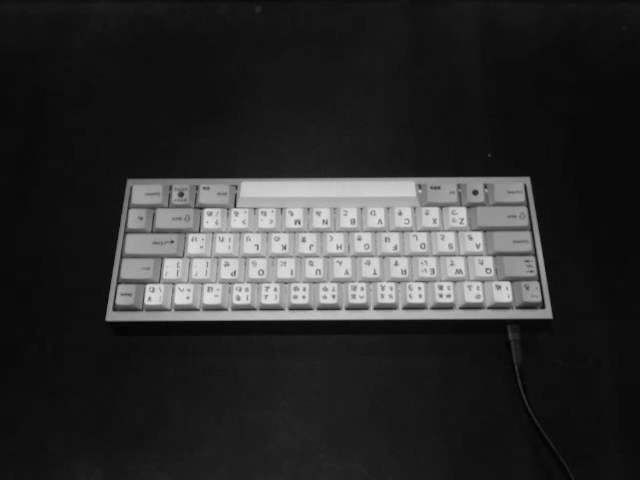
\includegraphics[width=0.8\textwidth]{grayscale.png}
	\caption{Camera capture converted to grayscale}
	\label{fig:metho-algo-convert}
	\centering
\end{figure}

\paragraph{Denoising}
The algorithm denoised the grayscale image using a bilateral filter as
implemented by OpenCV \parencite{opencv-bilateral-filter}. This filter takes the
range of the image into account, rather than just the domain. This resulted in
an image that is smoothed while preserving its edges
\parencite{bilateral-filter}. Figure~\ref{fig:metho-algo-denoise} is the output
of this step.

\begin{figure}[H]
	\centering
	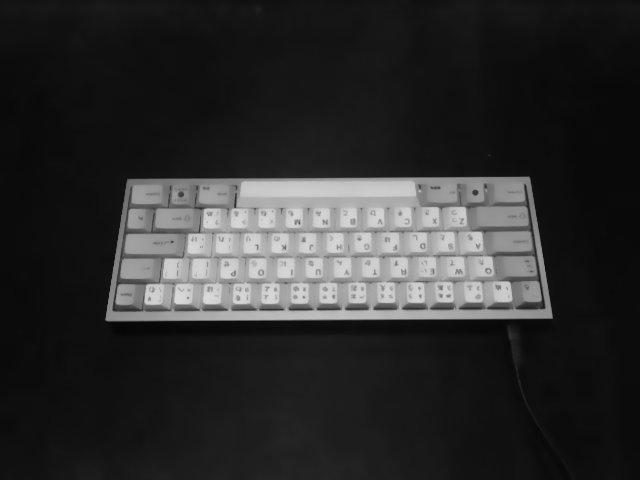
\includegraphics[width=0.8\textwidth]{denoised.png}
	\caption{Smoothed image with intact edges}
	\centering
	\label{fig:metho-algo-denoise}
\end{figure}


\paragraph{Edge Detection}
The algorithm used a Sobel filter for edge detection. This filter uses a
3$\times$3 kernel that is convolved twice --- once horizontally, and another
vertically --- to produce a grayscale image of the outlines within the frame.
The kernels used by the Sobel filter \parencite{sobel2014} is shown in
Figure~\ref{fig:metho-algo-key-sobel} and the output of this step is shown in
Figure~\ref{fig:metho-algo-sobel}.

\begin{figure}[H]
	\centering
	$\begin{bmatrix}
			+1 & 0 & -1 \\
			+2 & 0 & -2 \\
			+1 & 0 & -1
		\end{bmatrix}$
	$\begin{bmatrix}
			+1 & +2 & +1 \\
			0  & 0  & 0  \\
			-1 & -2 & -1
		\end{bmatrix}$
	\caption{Sobel Operator Kernels. Reproduced from \fullcite{sobel2014}}
	\label{fig:metho-algo-key-sobel}
\end{figure}

\begin{figure}[H]
	\centering
	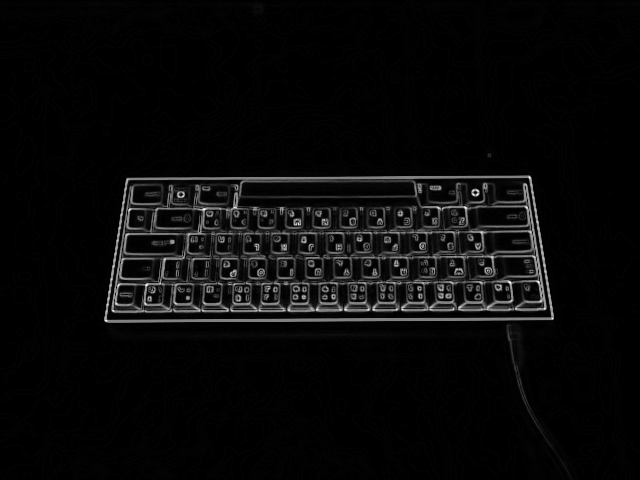
\includegraphics[width=0.8\textwidth]{sobel.png}
	\caption{Output of the Sobel filter}
	\centering
	\label{fig:metho-algo-sobel}
\end{figure}

\paragraph{Thresholding}
The output of the Sobel filter is a grayscale image of 256 values, with each
gray pixel indicating edges within the image. There is a need to reduce the
range of these values to improve the ability of the algorithm to find the
contours of these edges. To do so, the algorithm utilized Otsu's algorithm to
perform automated thresholding. Otsu's algorithm determines a single threshold
that is most optimal for the image \parencite{otsu}. This outputs a
black-and-white image, with only two values. Figure~\ref{fig:metho-algo-thresh}
is the resulting output of this step.

\begin{figure}[H]
	\centering
	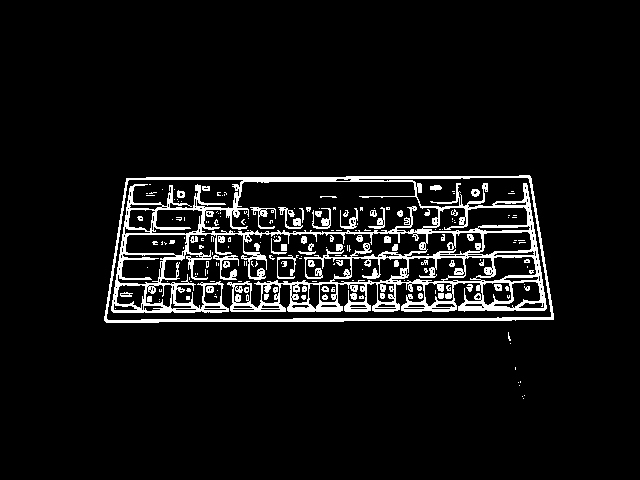
\includegraphics[width=0.8\textwidth]{threshed.png}
	\caption{Threshed image of the edges}
	\label{fig:metho-algo-thresh}
	\centering
\end{figure}


\paragraph{Find Contours}
\label{section:metho-algo-key-contours}
Contours are curves joining all continuous points that have the same color or
intensity \parencite{opencv-contours}. The OpenCV function
\texttt{findContours}, with the \texttt{CHAIN\_APPROX\_SIMPLE} contour
approximation method, was used to find the contours of the outlines of the
object found using the previous step. This approximation method removed
redundant points and returned the least amount of points that describe the
shape. This OpenCV function implements the algorithm of~\textcite{contours} in their
paper \citetitle{contours}. Figure~\ref{fig:metho-algo-contours} shows the contours
found in the threshed image.

\begin{figure}[H]
	\centering
	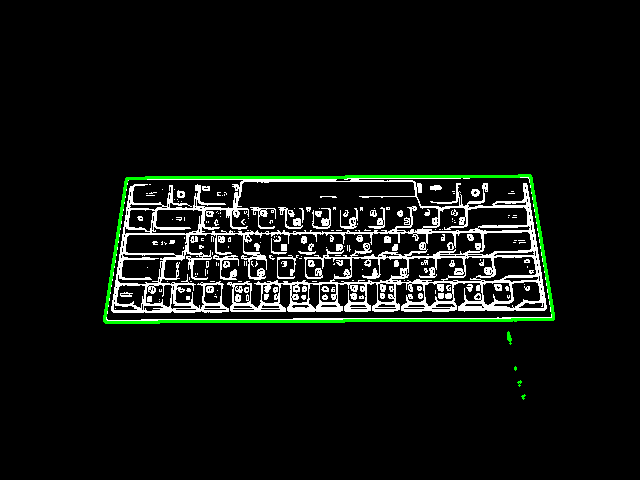
\includegraphics[width=0.8\textwidth]{find-contours.png}
	\caption{All the contours found in the image}
	\label{fig:metho-algo-contours}
	\centering
\end{figure}

\paragraph{Simplify Contour}
However, the points returned by the function can contain more than the four
extreme points at the edges of the keyboard. In addition, more than one contour
may be found within the image. As such, the algorithm sorted the contours by
area, and selected the largest one.

After sorting, the algorithm performed the Douglas-Peucker algorithm for Line
Simplification \parencite{douglas-peucker}. This reduced the number of points in
the largest contour to the minimum amount. In ideal cases, the number of points
would be four, with each point corresponding to the edges of the keyboard.
However, there were times when other objects would be within the frame, or they
intersected with the keyboard. This would result in a contour that would be
defined by more than four points --- which caused the entire algorithm to fail.

The contour points that described the contour were then sorted clockwise. This
was a necessity since the algorithm of~\textcite{contours} does not guarantee
that the largest contour's points were returned in a clockwise arrangement.
There is a need to have consistent ordering of these points since the
transformation that will be performed in the next step pairs the contour points
to a hard-coded array that indicates the edges of the image map. This hard-coded
array was sorted clockwise. As such, if the contour points were not sorted
clockwise, there will be no guarantee that the pairing would result in a
transformation that creates a transformed image map that is oriented correctly,
since the pairing may not pair the correct points.

Figure~\ref{fig:metho-algo-largest-contour} shows the four contour points found
at the edges of the keyboard within the image.

\begin{figure}[H]
	\centering
	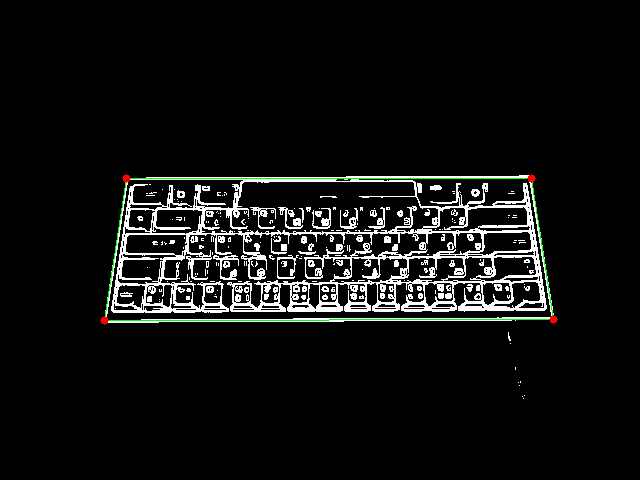
\includegraphics[width=0.8\textwidth]{get-largest-contour.png}
	\caption{Simplified contour}
	\label{fig:metho-algo-largest-contour}
	\centering
\end{figure}


\paragraph{Transform Image Map}
The virtual keyboard map is a rectangular image that contains individual
\ac{roi} for each key in a 60\% \ac{ansi} keyboard. Each key has a corresponding
color assigned to it and this color fills the region where this key is located
at. Figure~\ref{fig:metho-algo-key-map} is the initial image map and
Appendix~\ref{appendix:key-map} is a table that lays out the mapping of the
color code in BGR format and its associated character in the image map.

\begin{figure}[H]
	\centering
	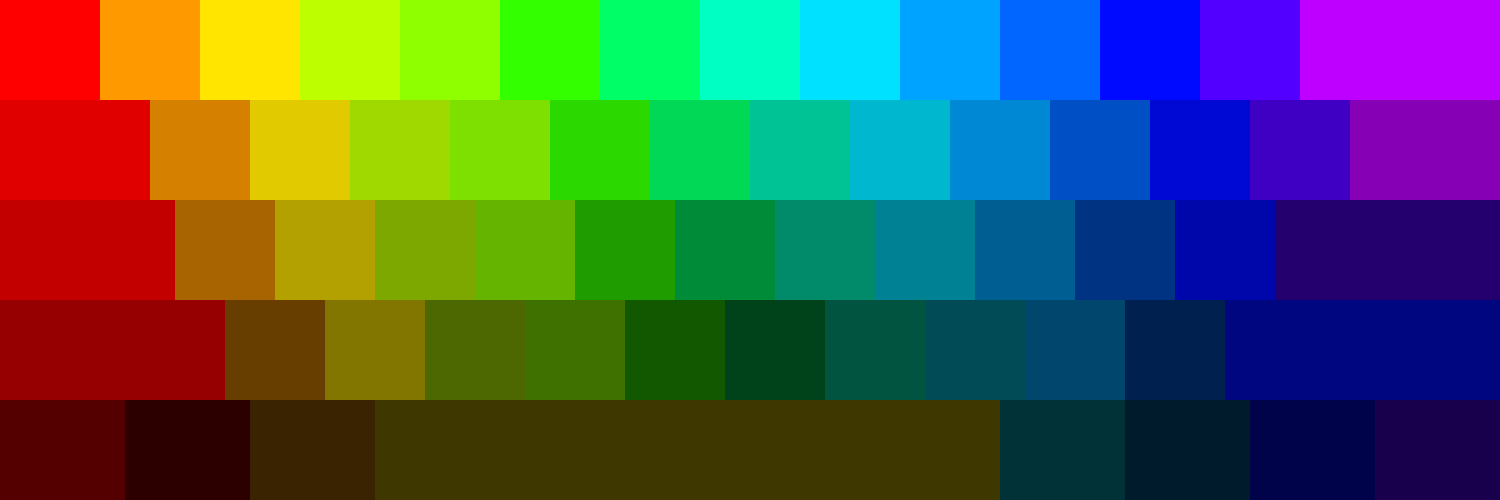
\includegraphics[width=0.6\textwidth]{image-map.png}
	\caption{Initial Image Map}
	\label{fig:metho-algo-key-map}
	\centering
\end{figure}

The virtual map was stretched over the keyboard using OpenCV's
\texttt{warpPerspective} function. The function requires a perspective transform
that was calculated using \texttt{getPerspectiveTransform}. This function takes
in two arrays with four points each. The input points are the edges of the
virtual map, ordered clockwise. The output points are the four points of the
contour, ordered clockwise \parencite{opencv-image-transform}. The resulting
transform was then used by \texttt{warpPerspective} to apply the transform to
the virtual map. Figure~\ref{fig:metho-algo-transform} is the image obtained
after warping the image map.

\begin{figure}[H]
	\centering
	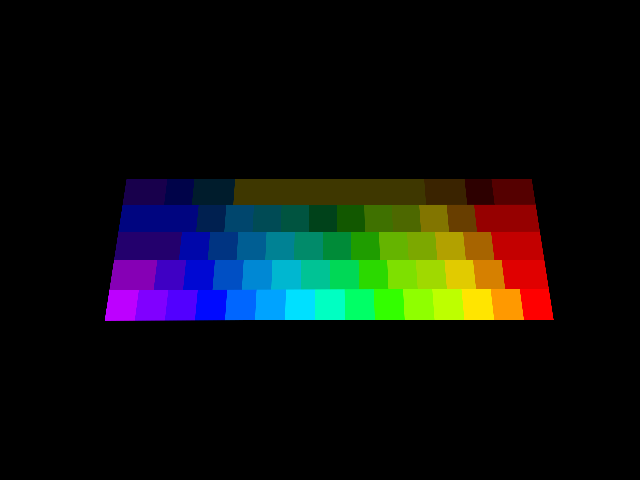
\includegraphics[width=0.6\textwidth]{transformed-image-map.png}
	\caption{Transformed image map}
	\label{fig:metho-algo-transform}
	\centering
\end{figure}

\subsubsection{Get Key Contour Points}
The second portion of the algorithm pre-computes the contour points of each key
in the keyboard based on the generated virtual map and the Key-Color Values map.
The flowchart of this function is shown in
Figure~\ref{fig:metho-algo-key-contour-points}

\begin{figure}[H]
	\centering
	\begin{tikzpicture}[font=\small,thick]
		\node[draw,
			rounded rectangle,
			minimum width = 2.5cm,
			minimum height = 1cm,
			inner sep = 3mm
		] (start) {START};

		\node[draw,
			trapezium,
			trapezium left angle = 65,
			trapezium right angle = 115,
			trapezium stretches,
			below = of start,
			minimum width = 3.5cm,
			minimum height = 1cm,
			align = center,
			inner sep = 3mm
		] (input) {Virtual Map \\ Key-Color Values Map};

		\node[draw,
			diamond,
			aspect = 2,
			below = of input,
			minimum width = 4cm,
			inner sep = 2mm] (for) {for Key, Color in Key-Color Values Map};

		\node[draw,
			below=of for,
			minimum width=3.5cm,
			minimum height=1cm,
			inner sep = 3mm
		] (filter) {Filter Virtual Map};

		\node[draw,
			below=of filter,
			minimum width=3.5cm,
			minimum height=1cm,
			inner sep = 3mm
		] (contours) {Find and Simplify Contour};

		\node[draw,
			below=of contours,
			minimum width=3.5cm,
			minimum height=1cm,
			inner sep = 3mm
		] (scale) {Scale Contours};

		\node[draw,
			trapezium,
			trapezium left angle = 65,
			trapezium right angle = 115,
			trapezium stretches,
			below=of scale,
			minimum width=3.5cm,
			minimum height=1cm,
			inner sep = 3mm
		] (output) {Key-Edge Coordinates Map};


		\node[draw,
			below=of output,
			rounded rectangle,
			minimum width=2.5cm,
			minimum height=1cm,
			inner sep = 3mm
		] (end) {END};

		\node[coordinate, right = 1cm of for] (top-right) {};
		\node[coordinate, right = 1cm of output] (below-right) {};
		\node[coordinate, left = 1cm of for] (top-left) {};
		\node[coordinate, left = 2cm of scale] (below-left) {};

		\draw[-latex] (start) edge (input)
		(input) edge (for)
		(for) edge (filter)
		(for) -- (top-right) -- (below-right) |- (output)
		(filter) edge (contours)
		(contours) edge (scale)
		(scale) -- (below-left) -- (top-left) |- (for)
		(output) edge (end);

	\end{tikzpicture}
	\caption{Flowchart of Get Key Contour Points}
	\label{fig:metho-algo-key-contour-points}
\end{figure}

\paragraph{Filter Virtual Map}
The color that corresponds to each key in the virtual map is stored in the
Key-Color Value Map. This color was used to create a mask for the virtual map
for a specific key. This mask was obtained by using this snippet of code
\texttt{(virtualMap == key).all(axis=2)}. This mask was then used to black out
the rest of the virtual map, leaving only the \ac{roi} of the key in the image.

This specific method was used as the other method that was trialed,
\texttt{np.where(virtualMap != key)}, did not consider all 3 channels when
comparing each pixel --- i.e.\ a key assigned with the color value of
\texttt{[100, 0, 0]} will not be blacked out if the color value of the key to be
isolated is \texttt{[100, 243, 0]} as the blue channel of the pixel,
\texttt{100} is equal in both. This would result in other keys remaining in the
virtual map, even if only one key corresponds to that color.
Figure~\ref{fig:metho-algo-filtered} shows the image where the Left Control key
was isolated.

\begin{figure}[H]
	\centering
	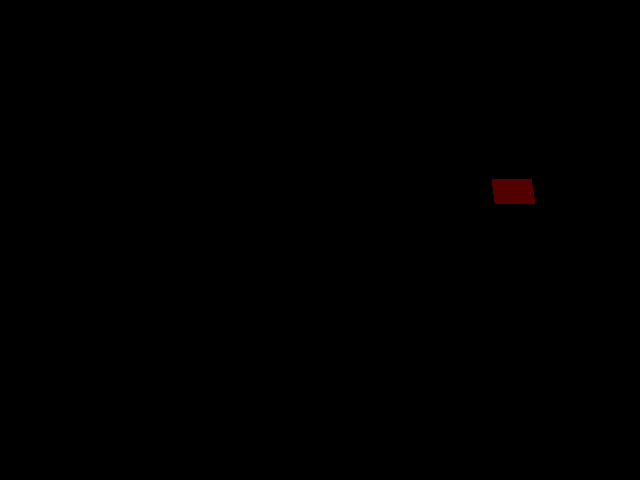
\includegraphics[width=0.8\textwidth]{filtered-key.png}
	\caption{Filtered key}
	\label{fig:metho-algo-filtered}
	\centering
\end{figure}

\paragraph{Find and Simplify Contours}
The same method in finding and simplifying the contour of the keyboard was used
to find and simplify the contour of the \ac{roi} of the key.
Figure~\ref{fig:metho-algo-contour-key} illustrates the four edges of the
isolated key.

\begin{figure}[H]
	\centering
	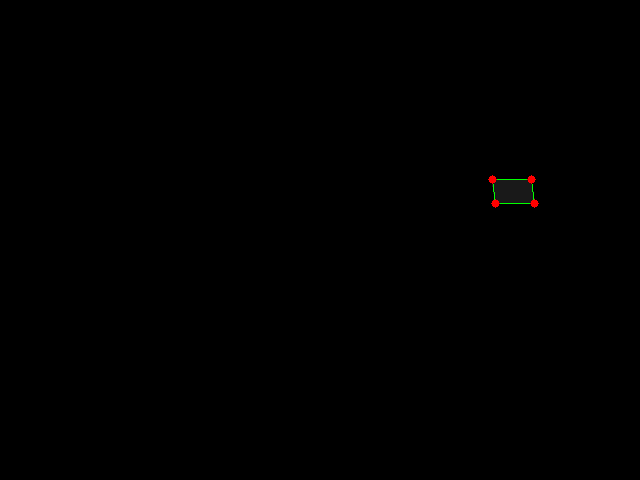
\includegraphics[width=0.8\textwidth]{key-contour.png}
	\caption{Contour points of the \ac{roi}}
	\label{fig:metho-algo-contour-key}
	\centering
\end{figure}

\paragraph{Scale Contours}
During testing using training data, a lot of the failures in finger-key
identification were due to the tight fit of the contour to the key. The contour
on its own did not give enough buffer for the placement of the finger. This
buffer was needed as, in some instances, the finger used to press the key was
not exactly on top of the key, but rather to its side. In addition, it can also
be observed that the finger tracking does not annotate the very edge of the
fingertip, but rather, it labels somewhere in the middle of the fingernail.

The algorithm accounts for this situation by adding a buffer. This was achieved
by scaling the contour points by seven pixels on each side.
Figure~\ref{fig:metho-algo-scale-roi} shows the increased buffer in relation to
the key. This value was obtained after testing other possible values. A buffer
of five pixels did not have a lot of effect in reducing the number of failures.
A buffer of ten pixels did reduce the number of failures, but it also greatly
increased the algorithm's uncertainty in determining the finger --- uncertainty
is defined as detecting two or more fingers within one \ac{roi}. Seven was a
good middle ground in decreasing failures, without greatly increasing
uncertainty.

\begin{figure}[H]
	\centering
	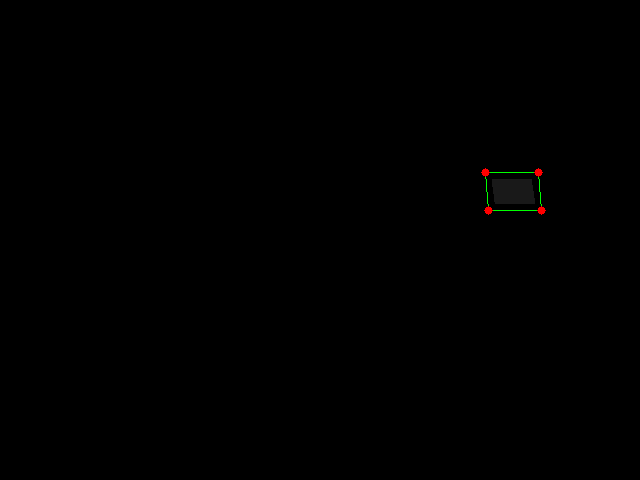
\includegraphics[width=0.8\textwidth]{scaled-contour.png}
	\caption{Scaled contour points of the \ac{roi} with the buffer of seven pixels}
	\label{fig:metho-algo-scale-roi}
	\centering
\end{figure}

\paragraph{Key-Edge Coordinates Map}
After all the keys have passed through the loop, a Key-Edge Coordinates Map was
generated. Each key now has four points that serve as the coordinates of the
edge of its \ac{roi}.

The coordinate system that the contour points are based on had its origin at the
top left, starting at 0, 0. Going to the right increased the value of the
x-axis, and going to the bottom increased the value of the y-axis. This results
in a coordinate system that only has positive values with each value
corresponding to a pixel.


\subsection{Computer Vision based Finger Detection, and Tracking}
\label{section:metho-algo-finger}
MediaPipe Hands was used as the finger detection and tracking solution. This
algorithm is composed of two ML models working in conjunction to be able to
detect the different parts of the hands and track them accurately.

\subsubsection{Palm Detection Model}
The first model, the Palm Detection Model detects the initial hand locations
using a single shot detector model based on the paper by~\textcite{ssd}. This model
achieves an average precision of 95.7\% in palm detection
\parencite{mediapipe-hands}.

MediaPipe Hands detects the palms first, instead of whole hands with one model
because hands lack high contrast patterns. This reduces the model's ability to
detect hands with accuracy. In addition, detecting a palm is simpler compared
to detecting hands with articulated fingers since estimating a bounding box
around a rigid object, i.e.\ a palm is much simpler. Furthermore, a palm can be
modeled using only square anchors reducing the number of anchors by a factor of
3--5 \parencite{mediapipe-hands}.

\subsubsection{Hand Landmark Model}
After the palms have been detected and an appropriate anchor has been
established, the Hand Landmark Model pinpoints 21 3D hand-knuckle coordinates
inside the detected hand. This is done using direct coordinate prediction.

This model was trained using 30,000 manually annotated, real-world images with
21 3D hand-knuckle coordinates. Using this information, the model can also
accurately add landmarks to partially visible hands and hands with
self-occlusion. This is also made possible by the model's consistent internal
hand pose representation \parencite{mediapipe-hands}.

\subsection{Integration for finger-key identification and mapping}

The two previously chosen algorithms were combined to accomplish finger-key
identification and mapping.

The integration of the algorithm was a two-step process. The first step was to
get the Key-Edge Coordinates Map shown in
Section~\ref{section:metho-algo-keyboard}.

The second step runs whenever a key press has been detected. This step used the
Key-Edge Coordinates Map in conjunction with the finger tracking algorithm selected
in Section~\ref{section:metho-algo-finger}. The flowchart of the algorithm is
shown in Figure~\ref{fig:metho-algo-integration}

\begin{figure}[H]
	\centering
	\tikzset{
		rectangle connector/.style={
				-latex,
				to path={(\tikztostart) -- ++(6cm,0pt) \tikztonodes |- (\tikztotarget) },
				pos=0.5
			},
	}
	\begin{tikzpicture}[font=\small,thick]
		\node[draw,
			rounded rectangle,
			minimum width = 2.5cm,
			minimum height = 1cm,
			inner sep = 3mm
		] (start) {START};

		\node[draw,
			diamond,
			aspect = 2,
			below = of start,
			minimum width = 4cm,
			inner sep = 3mm] (if-packet) {Keypress Detected};

		\node[draw,
			trapezium,
			trapezium left angle = 65,
			trapezium right angle = 115,
			trapezium stretches,
			below = 2cm of if-packet,
			minimum width = 3.5cm,
			minimum height = 1cm,
			align = center,
			inner sep = 3mm
		] (map) {Key-Edge Coordinates Map \\ Finger Tracking Data};

		\node[draw,
			below=of map,
			minimum width = 3.5cm,
			minimum height = 1cm,
			inner sep = 3mm
		] (find-finger) {Find which fingertip is on that \ac{roi}};

		\node[draw,
			trapezium,
			trapezium left angle = 65,
			trapezium right angle = 115,
			trapezium stretches,
			below = of find-finger,
			minimum width = 3.5cm,
			minimum height = 1cm,
			inner sep = 3mm
		] (return) {Return which fingertip};

		\node[draw,
			below = of return,
			rounded rectangle,
			minimum width = 2.5cm,
			minimum height = 1cm,
			inner sep = 3mm
		] (end) {END};

		\draw[-latex] (start) edge (if-packet)
		(map) edge (find-finger)
		(find-finger) edge (return)
		(return) edge (end);

		\draw[-latex] (if-packet) edge node[pos=0.5, fill=white, inner sep=2] {true} (map);
		\draw[rectangle connector] (if-packet) to node[fill=white, inner sep=2] {false} (end);

	\end{tikzpicture}
	\caption{Flowchart of the overall flow}
	\label{fig:metho-algo-integration}
\end{figure}

\subsubsection{Find which fingertip is on that \ac{roi}}
The Finger Tracking Data contained the pixel positions of each landmark of the
hand. For this step, the algorithm finds the landmark which is positioned within
the single \ac{roi} obtained from the previous step. This was done using a
series of checks.

Each landmark's coordinates were compared to the coordinates of the edges of the
\ac{roi}. A landmark was determined as positioned within the \ac{roi} if all the
following conditions are true:

\begin{enumerate}
	\item On the X-axis, the landmark's coordinates are greater than one or both of
	      the two coordinates found on the left side of the \ac{roi}
	\item On the X-axis, the landmark's coordinates are less than one or both of
	      the two coordinates found on the right side of the \ac{roi}
	\item On the Y-axis, the landmark's coordinates are greater than one or both of
	      the two coordinates found on the top side of the \ac{roi}
	\item On the Y-axis, the landmark's coordinates are less than one or both of
	      the two coordinates found of the bottom side of the \ac{roi}
\end{enumerate}

These conditions maximized the total area of the \ac{roi}, and it is not strict
about exact accuracy. In essence, these conditions create a perfectly
rectangular box that contained the quadrilateral formed by the four points from
the coordinates. Figure~\ref{fig:metho-algo-sample} is an example of a frame with a
successful finger-key identification using the conditions previously mentioned.

\begin{figure}[H]
	\centering
	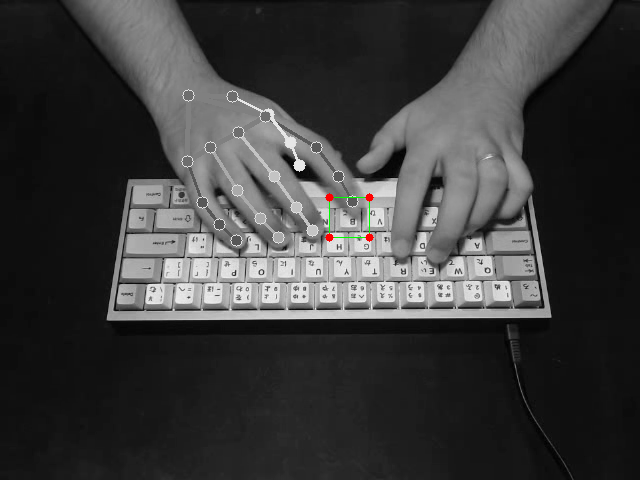
\includegraphics[width=0.8\textwidth]{detected-finger.png}
	\caption{Fingertip within an \ac{roi}}
	\label{fig:metho-algo-sample}
	\centering
\end{figure}

\subsubsection{Return which fingertip}
The landmark was then used to determine which specific finger corresponds to the
key press. Figure~\ref{fig:metho-algo-integration-landmarks} shows each possible
landmark that may be returned from the previous step. This step returned the
name of the landmark, up until the first underscore. As an example, if the
landmark found is \texttt{MIDDLE\_FINGER\_TIP}, this step will return
\texttt{MIDDLE} denoting that the middle finger is the finger that corresponds
with the key press. In addition, the specific hand will also be returned as one
of two strings, \texttt{LEFT} and \texttt{RIGHT}, since this information is also
bundled together with the landmarks. The two strings were then concatenated with
an underscore. An example return value is \texttt{RIGHT\_RING}.

As such, the expected output of the module is the hand and the finger used to
press the key. This allows for a more flexible utilization of the data as it
carries greater context, compared to just returning if the finger used was
correct or not.

\begin{figure}[H]
	\centering
	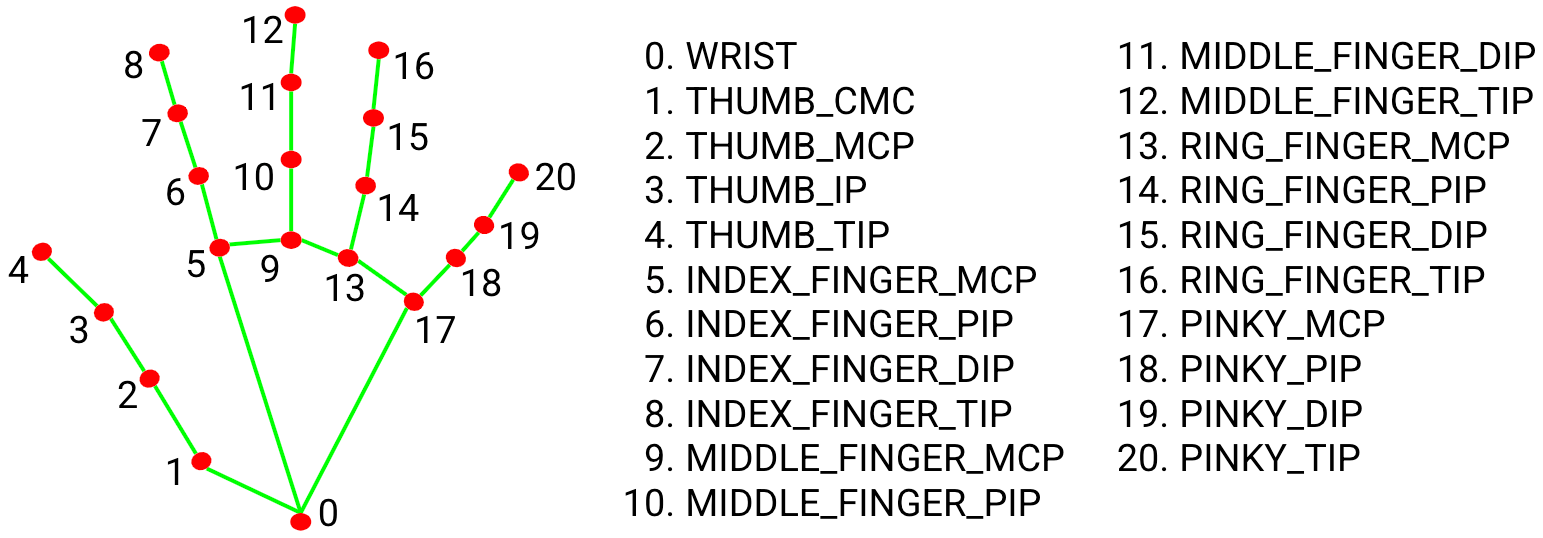
\includegraphics[width=0.6\textwidth]{hand-landmarks.png}
	\caption{Hand landmarks that may be returned by the algorithm. Reproduced from \fullcite{mediapipe-hands}}.
	\label{fig:metho-algo-integration-landmarks}
	\centering
\end{figure}

\subsection{Implementation}
\label{section:metho-algo-implementation}
The previously discussed algorithms were implemented using Python. The Keyboard
Detection and Mapping Algorithm in Section~\ref{section:metho-algo-keyboard} was
implemented as a separate module in Python using OpenCV. The Finger Detection
and Tracking Solution in Section~\ref{section:metho-algo-finger} was implemented
using the prebuilt Python package offered by the MediaPipe team. Finally, the
integration of the two was done as another separate module in Python.

\section{Training and Testing}

\subsection{Typing Test Sequences}
Typing test sequences are strings that were used in testing the user in their
ability to type. The test sequences that were used came from text found in the
public domain obtained from Project Gutenberg and the Internet Archive.
Sentences were isolated from these texts and used as test sequences if they fit
the criteria.

The criteria for choosing test sequences were as follows: (1) $\approx80\%$ of
the characters on the keyboard is present in a test sequence. (2) The number of
words in a test sequence does not exceed 25. (3) Numbers and punctuations should
be present in at least $\approx30\%$ of the total test sequences.

There was a total of 10 test sequences that were gathered. An example test
sequence is ``What of it, if some old hunks of a sea-captain orders me to get a
broom and sweep down the decks?'' from Moby Dick by~\textcite{moby-dick}. The 9
other test sequences can be found in Appendix
Chapter~\ref{appendix:test-sequences}.

\subsection{Data Gathering}
\subsubsection{Video Capture}
There were 3 sets of 10 videos that were captured by the researcher, for a total
of 30 videos. Each set corresponds to three predetermined speeds of typing: slow
(15wpm), average (35wpm), and fast (80wpm). These speeds were based on test data
from~\textcite{keybr}. The researcher typed the 10 typing test sequences at
these predetermined speeds. Best effort was made to stick to the predetermined
speeds. During typing, errors were not consciously taken into account, and
errors happened naturally as part of the typing process --- with more errors
happening more frequently as the typing speed increased.

A Python script was created to facilitate this process. The script captured a
video of the researcher as the researcher was typing the test sequences.
Whenever the researcher pressed a key, the corresponding frame count was
captured, and the key pressed was recorded in conjunction. This was stored in
the format \texttt{FRAME\_NO:KEY\_PRESSED}, and each keypress was then stored as
a line in a file.

One caveat of the camera used was its autofocus capabilities. This meant that
there was a set amount of time during the start of the recording where the
camera captured blurry images of the keyboard. This necessitates around three
seconds for the autofocus to complete and focus on the keyboard. There was one
video capture where the whole test sequence was scrapped as the researcher
started typing even if the camera was not focused.

\subsubsection{Keypress Labeling}
The researcher then manually performed finger-key identification for all key
presses present in the video. This was also done through a Python script. The
script parsed the file associated with a video. The frame number found at each
line was then shown, and the associated data with the frame was superimposed
over it. Figure~\ref{fig:metho-data-process} is an example of a frame with these
data overlaid over the captured image. The researcher then pressed keys that
corresponded with the finger used to press the key. This was then again stored
in the format \texttt{FRAME\_NO:KEY\_PRESSED:FINGER\_USED}, and each keypress
was then stored as a line in a file.

\begin{figure}[H]
	\centering
	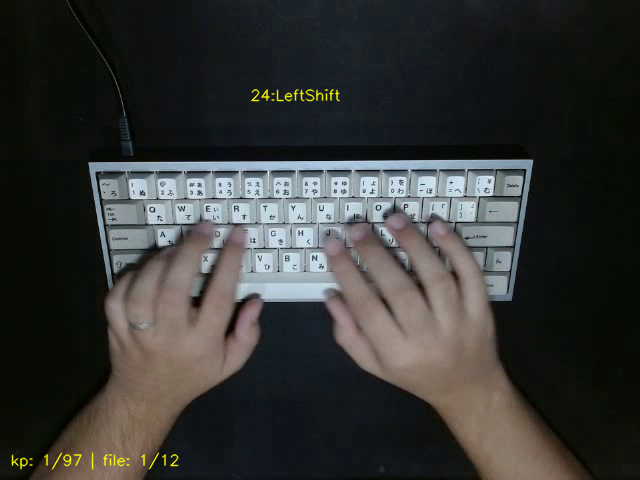
\includegraphics[width=0.6\textwidth]{labeling.png}
	\caption{Screen showing the labeling process}
	\label{fig:metho-data-process}
	\centering
\end{figure}


\subsubsection{Test-Training Split}
The annotated data was then divided into training and test data at a ratio of
60:40.

\subsubsection{Data Inventory}

\begin{figure}[H]
	\centering
	\begin{tikzpicture}
		\begin{axis}[
				xbar, xmin=0,
				bar width=4pt,
				width=0.8\textwidth,
				ylabel=Key,
				xlabel=Count,
				symbolic y coords={
						J,
						Q,
						Dash,
						ForwardSlash,
						Z,
						1,
						LeftAlt,
						X,
						Comma,
						K,
						V,
						G,
						B,
						Backspace,
						W,
						Period,
						P,
						U,
						C,
						LeftShift,
						F,
						Y,
						M,
						H,
						D,
						L,
						I,
						R,
						N,
						T,
						S,
						A,
						O,
						E,
						Spacebar,
					},
				ytick=data,
				tick label style={font=\footnotesize},
				label style={font=\footnotesize},
				xmajorgrids=true
			]
			\addplot table[x=Value,y=Key]{training-data.txt};
		\end{axis}
	\end{tikzpicture}
	\caption{Training Dataset Inventory}
	\label{fig:metho-inventory-training}
\end{figure}

Individual counts of the characters in the training iteration data set is shown
in Figure~\ref{fig:metho-inventory-training}. The letters were not represented
equally in the data set. Of note, J and Q were not in the dataset.

\begin{figure}[H]
	\centering
	\begin{tikzpicture}
		\begin{axis}[
				xbar, xmin=0,
				bar width=4pt,
				width=0.8\textwidth,
				ylabel=Key,
				xlabel=Count,
				symbolic y coords={
						J,
						Q,
						Z,
						Dash,
						ForwardSlash,
						X,
						V,
						Period,
						K,
						B,
						Comma,
						G,
						F,
						Backspace,
						P,
						W,
						C,
						U,
						M,
						Y,
						D,
						LeftShift,
						L,
						H,
						N,
						R,
						S,
						I,
						O,
						A,
						T,
						E,
						Spacebar,
					},
				ytick=data,
				tick label style={font=\footnotesize},
				label style={font=\footnotesize},
				xmajorgrids=true
			]
			\addplot table[x=Value,y=Key]{test-data.txt};
		\end{axis}
	\end{tikzpicture}
	\caption{Test Dataset Inventory}
	\label{fig:metho-inventory-test}
\end{figure}

The letters were also not represented equally in the test dataset as shown in
Figure~\ref{fig:metho-inventory-test}. Three characters in the alphabet were not
represented in the dataset: J, Q, and Z. The inequality of representation in
both of these datasets can be attributed to the source materials of the typing
test sequences --- novels and texts. While there were criteria to select which
text was sourced, there was no conscious decision to equally represent all
characters in the data set.

\subsection{Training}
A script was created to test the accuracy of the module. This script opened each
video and the associated labeled file. There were three frames taken for each
video to perform step one of the module: frames ten, fifteen, and twenty. The
first frame that returned a Key-Edge Coordinates Map after going through step
one of the module was used. The rest of the frames were not passed through the
module and were discarded.

The script then parsed the labeled file and opened the frame for each keypress.
The second algorithm of the module was then run, using the data needed for the
algorithm: the key pressed. The result of the module was then compared with the
manual labeling of the keypress. The resulting data from the test was then
stored in a \texttt{.csv} file with the following content:

\begin{table}[H]
	\small
	\centering
	\caption{\label{tab:csv-output}CSV File Contents}
	\begin{tabular}{ p{0.3\textwidth} p{0.6\textwidth} }
		\toprule
		Column Name                           & Definition                                             \\
		\midrule
		\texttt{file\_name}                   & Name of the file                                       \\
		\texttt{frame}                        & Frame number                                           \\
		\texttt{key}                          & Key pressed                                            \\
		\texttt{finger}                       & Manual labeling of the finger used to press the key    \\
		\texttt{is\_correct}                  & If the module was correct                              \\
		\texttt{fingertips\_detected}         & The fingertips detected by the module                  \\
		\texttt{keyboard\_detection\_time}    & Time spent in creating the Key-Edge Coordinates Map    \\
		\texttt{finger\_classification\_time} & Time spent in classifying which finger pressed the key \\
		\bottomrule
	\end{tabular}
\end{table}

Adjustments were then made to the algorithm after each training pass to improve
its performance. Some runs had improvements in their statistics without doing
any adjustments. These were runs that showed errors in the manual labeling and
were corrected afterward.

\subsection{Analysis}
The resulting \texttt{.csv} file was imported into Google Sheets and key
statistics were obtained based on the data. Appendix~\ref{appendix:sheets} shows
the screenshots where this was performed. The statistics obtained can be found
in Table~\ref{tab:acquired-stats}. These key statistics informed what to adjust
in the algorithm and its overall performance.

\begin{table}[H]
	\small
	\centering
	\caption{\label{tab:acquired-stats}Acquired statistics}
	\begin{tabular}{ p{0.3\textwidth} p{0.6\textwidth} }
		\toprule
		Identifications                                                                                                                    \\
		\midrule
		Successes                                & Number of successful finger-key identifications                                         \\
		Failures                                 & Number of failed finger-key identifications                                             \\
		Success Percentage                       & Percentage of successful finger-key identifications                                     \\
		Failure Percentage                       & Percentage of failed finger-key identifications
		\\[0.25cm]
		\midrule
		Failure Types                                                                                                                      \\
		\midrule
		Mismatched Identification                & Module output did not match manual labeling                                             \\
		No Identification                        & Module did not detect fingertips in \ac{roi}
		\\[0.25cm]
		\midrule
		Uncertain Successes                                                                                                                \\
		\midrule
		Total                                    & Total uncertain successes, defined as detecting two or more fingers within one \ac{roi} \\
		Spacebar                                 & All uncertain successes that were on the spacebar                                       \\
		Spacebar Percentage                      & Percentage of spacebar uncertain successes over all uncertain successes                 \\
		Spacebar Percentage (Total)              & Percentage of spacebar uncertain successes over total keypresses                        \\
		Non-spacebar                             & All other uncertain successes                                                           \\
		Non-spacebar Percentage                  & Percentage of non-spacebar uncertain successes over all uncertain successes             \\
		Non-spacebar Percentage \newline (Total) & Percentage of non-spacebar uncertain successes over total keypresses
		\\[0.25cm]
		\midrule
		Average Running Time                                                                                                               \\
		\midrule
		Keyboard Detection Time                  & Average keyboard detection time of all videos                                           \\
		Finger Identification Time               & Average finger identification time of all key presses                                   \\
		\bottomrule
	\end{tabular}
\end{table}

\subsection{Testing}
The same script was run through the test data. The same format of output was
gathered, and the same key statistics were recorded.

\section{Trainer}
A trainer was developed as a proof of concept of a real-world implementation of
the finger-key identification module.

\subsection{Design}
The design was heavily based on Monkeytype by \textcite{bartnik2021}. Additional
components were added to enable real-time finger-key identification. There are
three main screens:

\begin{figure}[H]
	\centering
	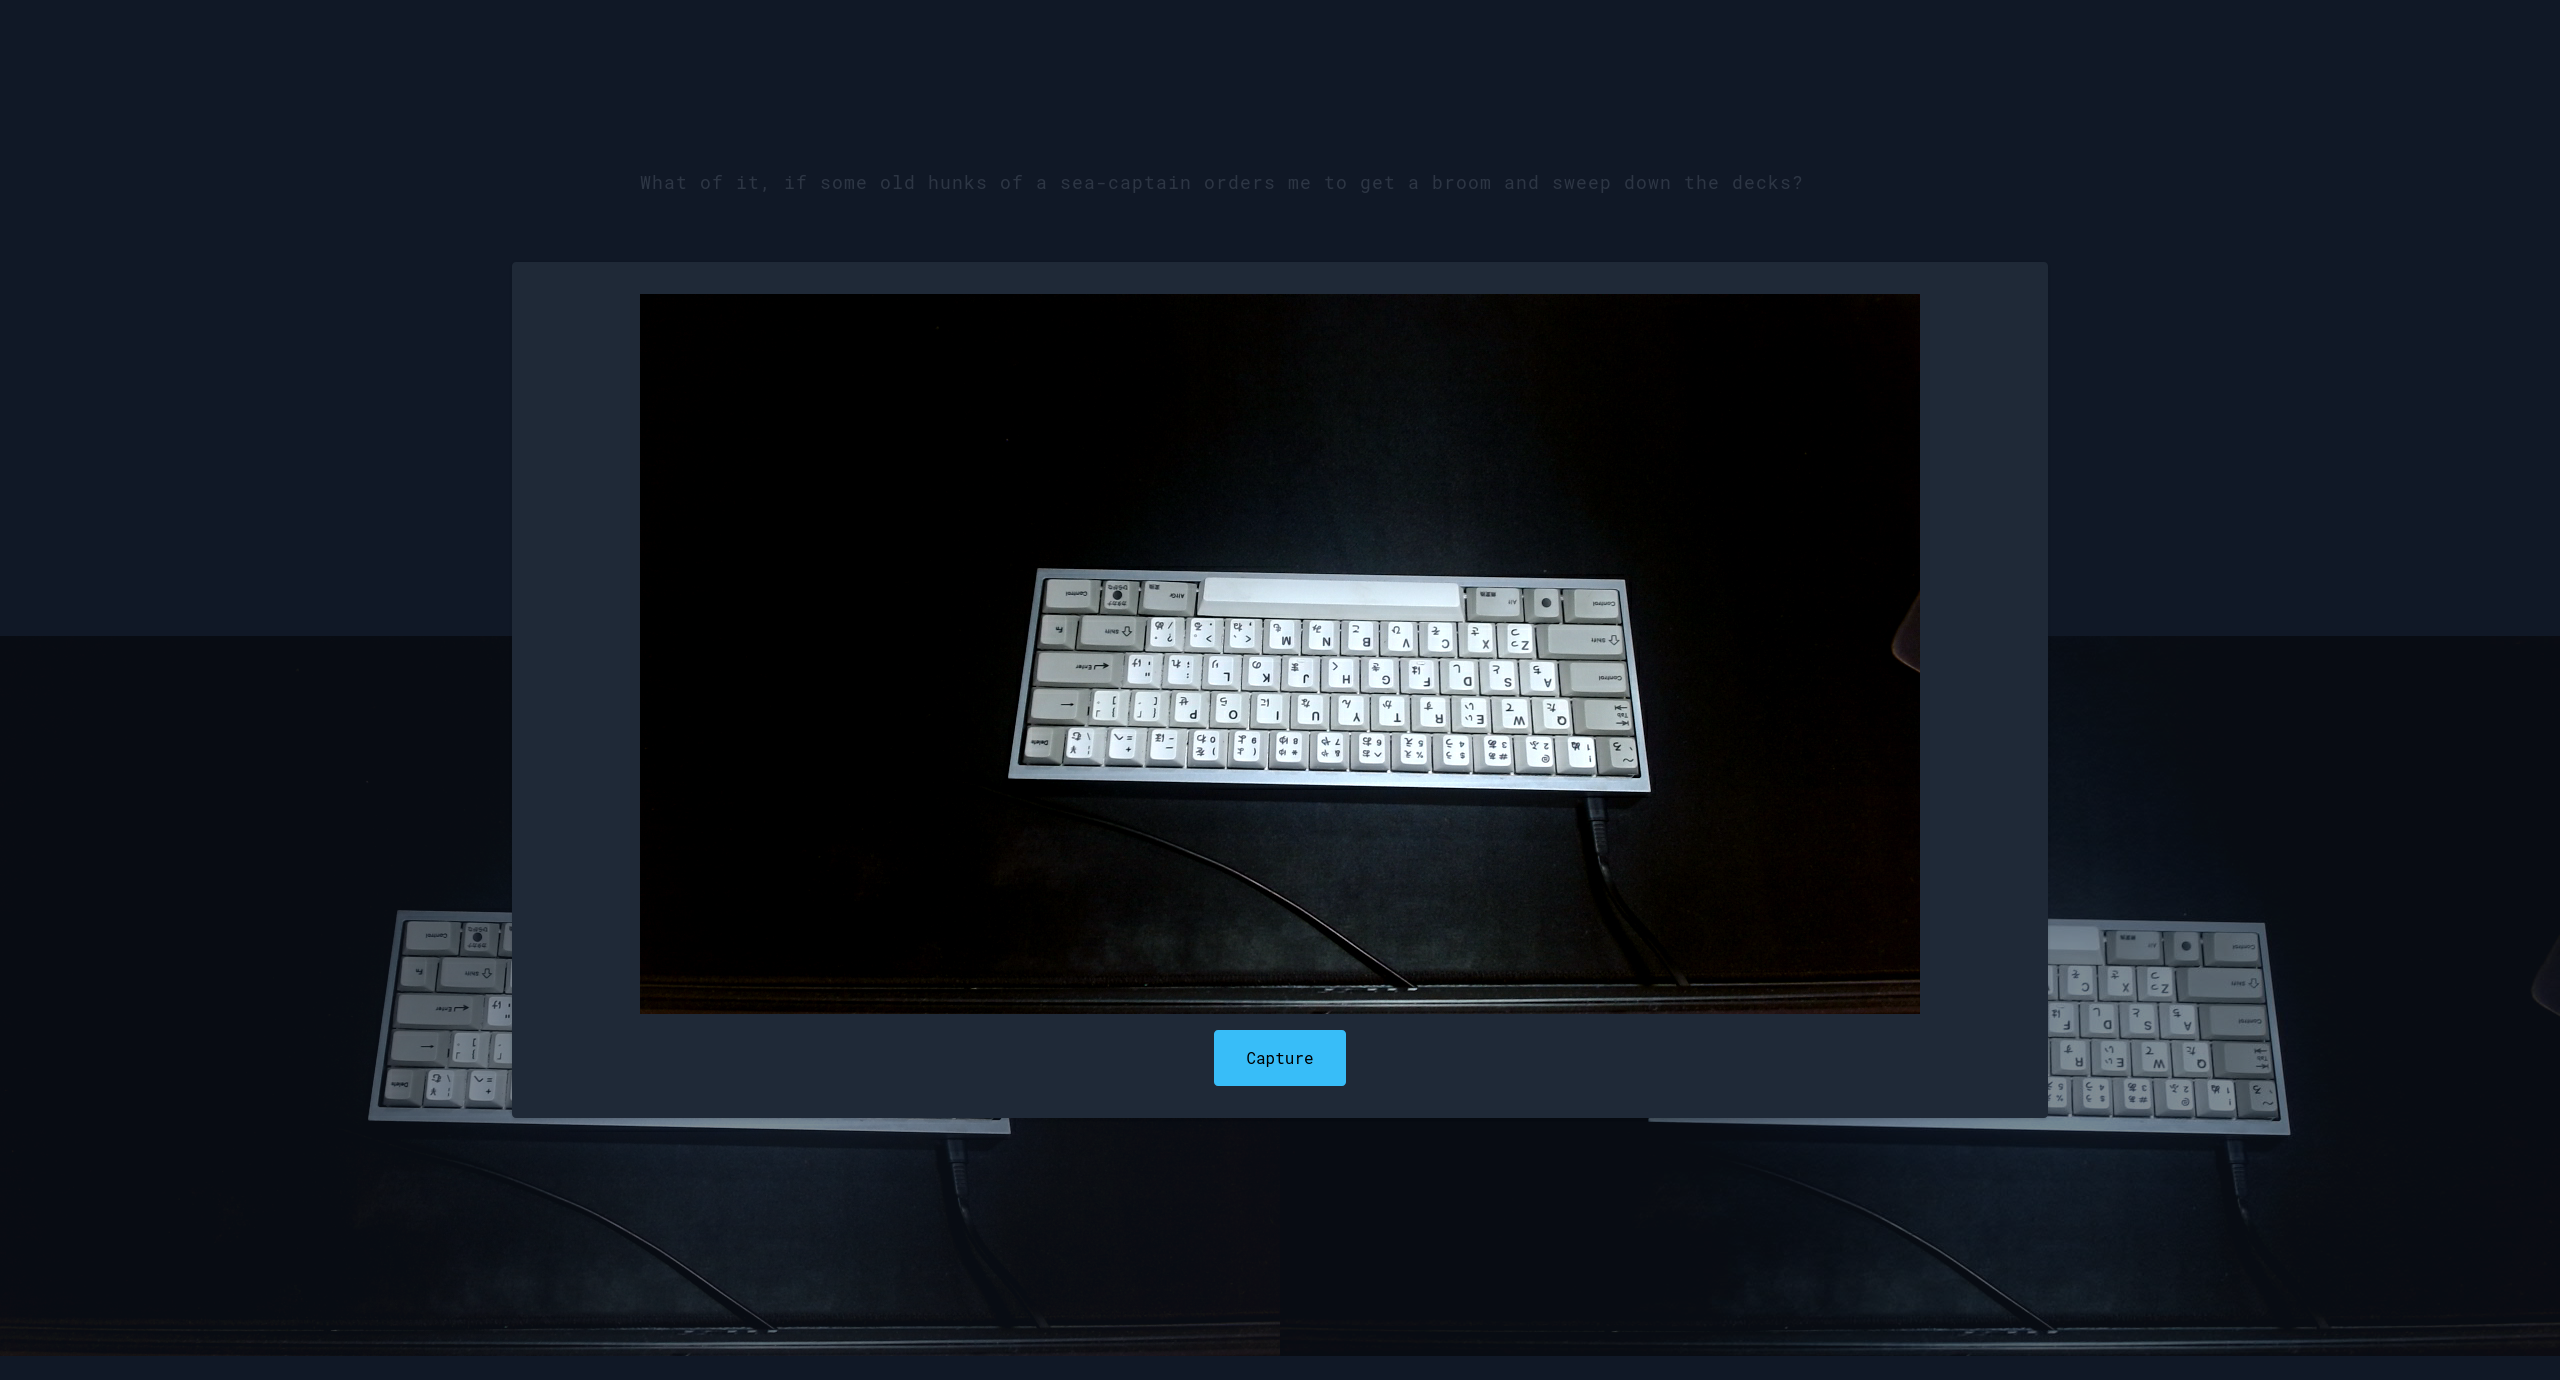
\includegraphics[width=1\textwidth]{frontend-edge-coords.png}
	\caption{Frontend Screen for obtaining Key-Edge Coordinates Map}
	\label{fig:metho-front-coords}
	\centering
\end{figure}

Figure~\ref{fig:metho-front-coords} shows the first screen the user sees. This page
captured the keyboard and passed it to the backend to obtain the Key-Edge
Coordinates Map.

\begin{figure}[H]
	\centering
	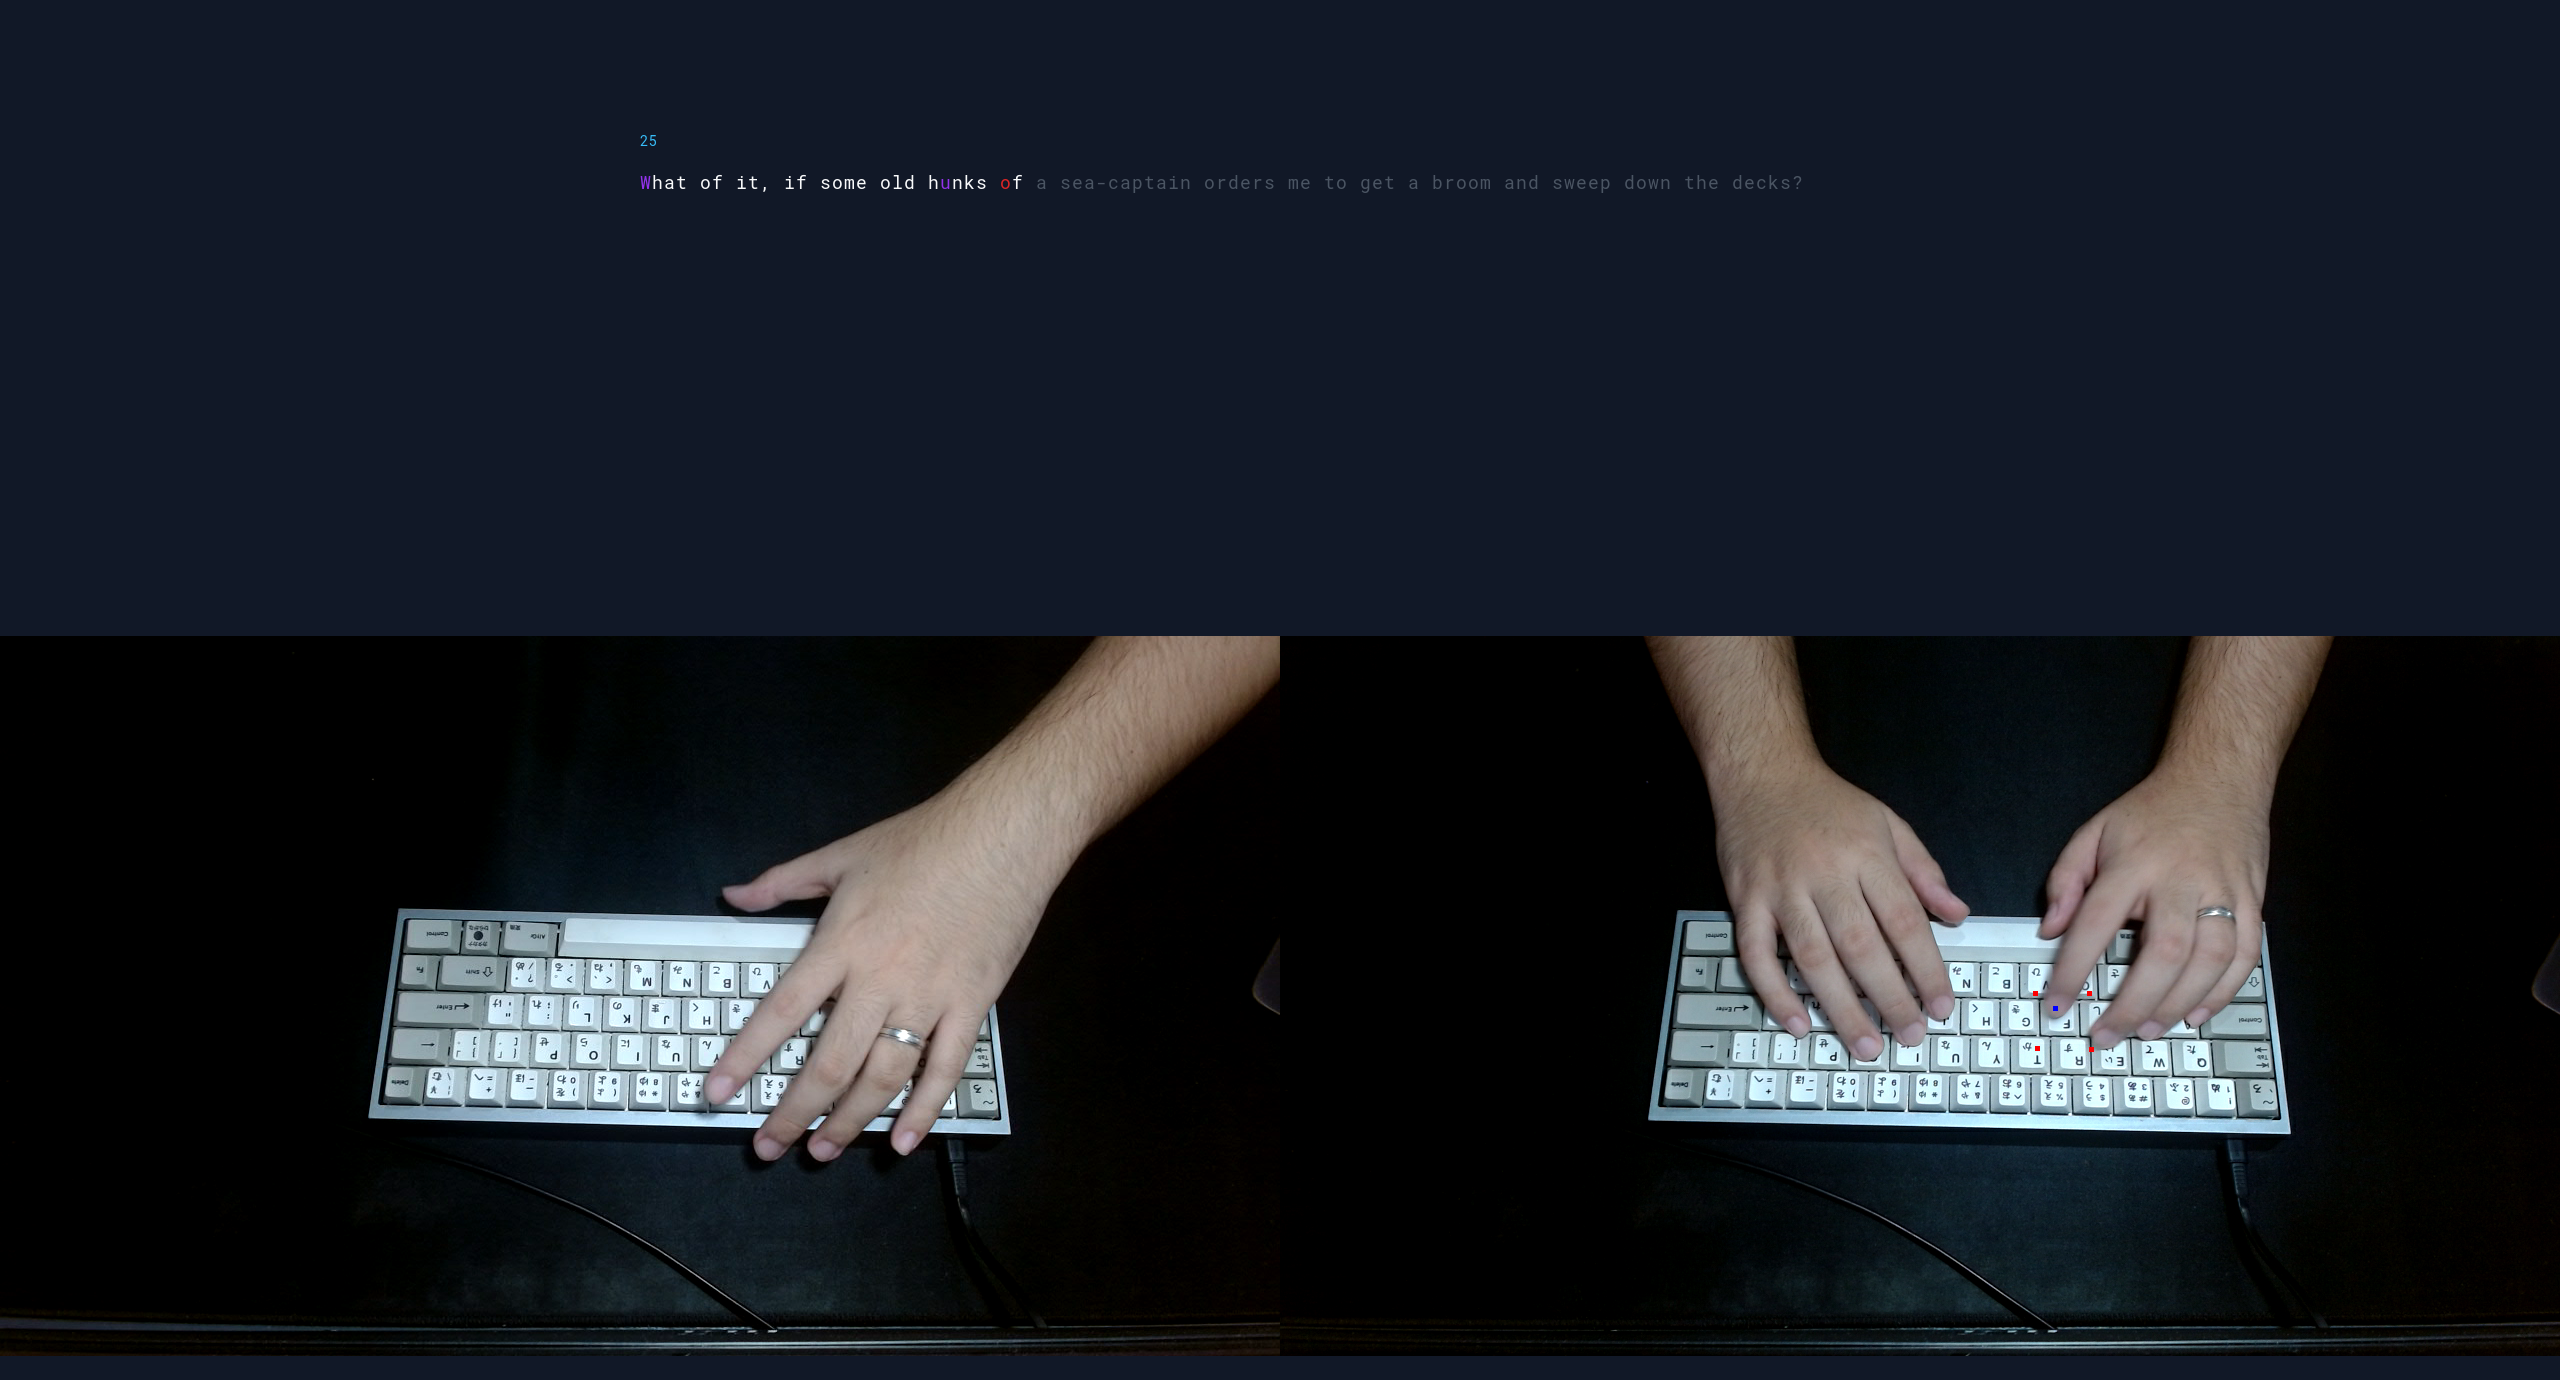
\includegraphics[width=1\textwidth]{frontend-test.png}
	\caption{Testing page of the trainer}
	\label{fig:metho-front-test}
	\centering
\end{figure}

Figure~\ref{fig:metho-front-test} is the screen where the user performs the
typing test. On this screen, the typing test sequence was placed above. If a
letter was typed correctly with the correct finger, the character was colored
white. If the wrong character was typed, the character was colored red. If the
correct character was typed, but the finger used was incorrect, the character
was colored purple.

At the bottom, the video captured by the webcam was shown on the left. Right
beside it, important coordinates of the finger-key identification module are
overlaid over the specific frame that was used as the input.

\begin{figure}[H]
	\centering
	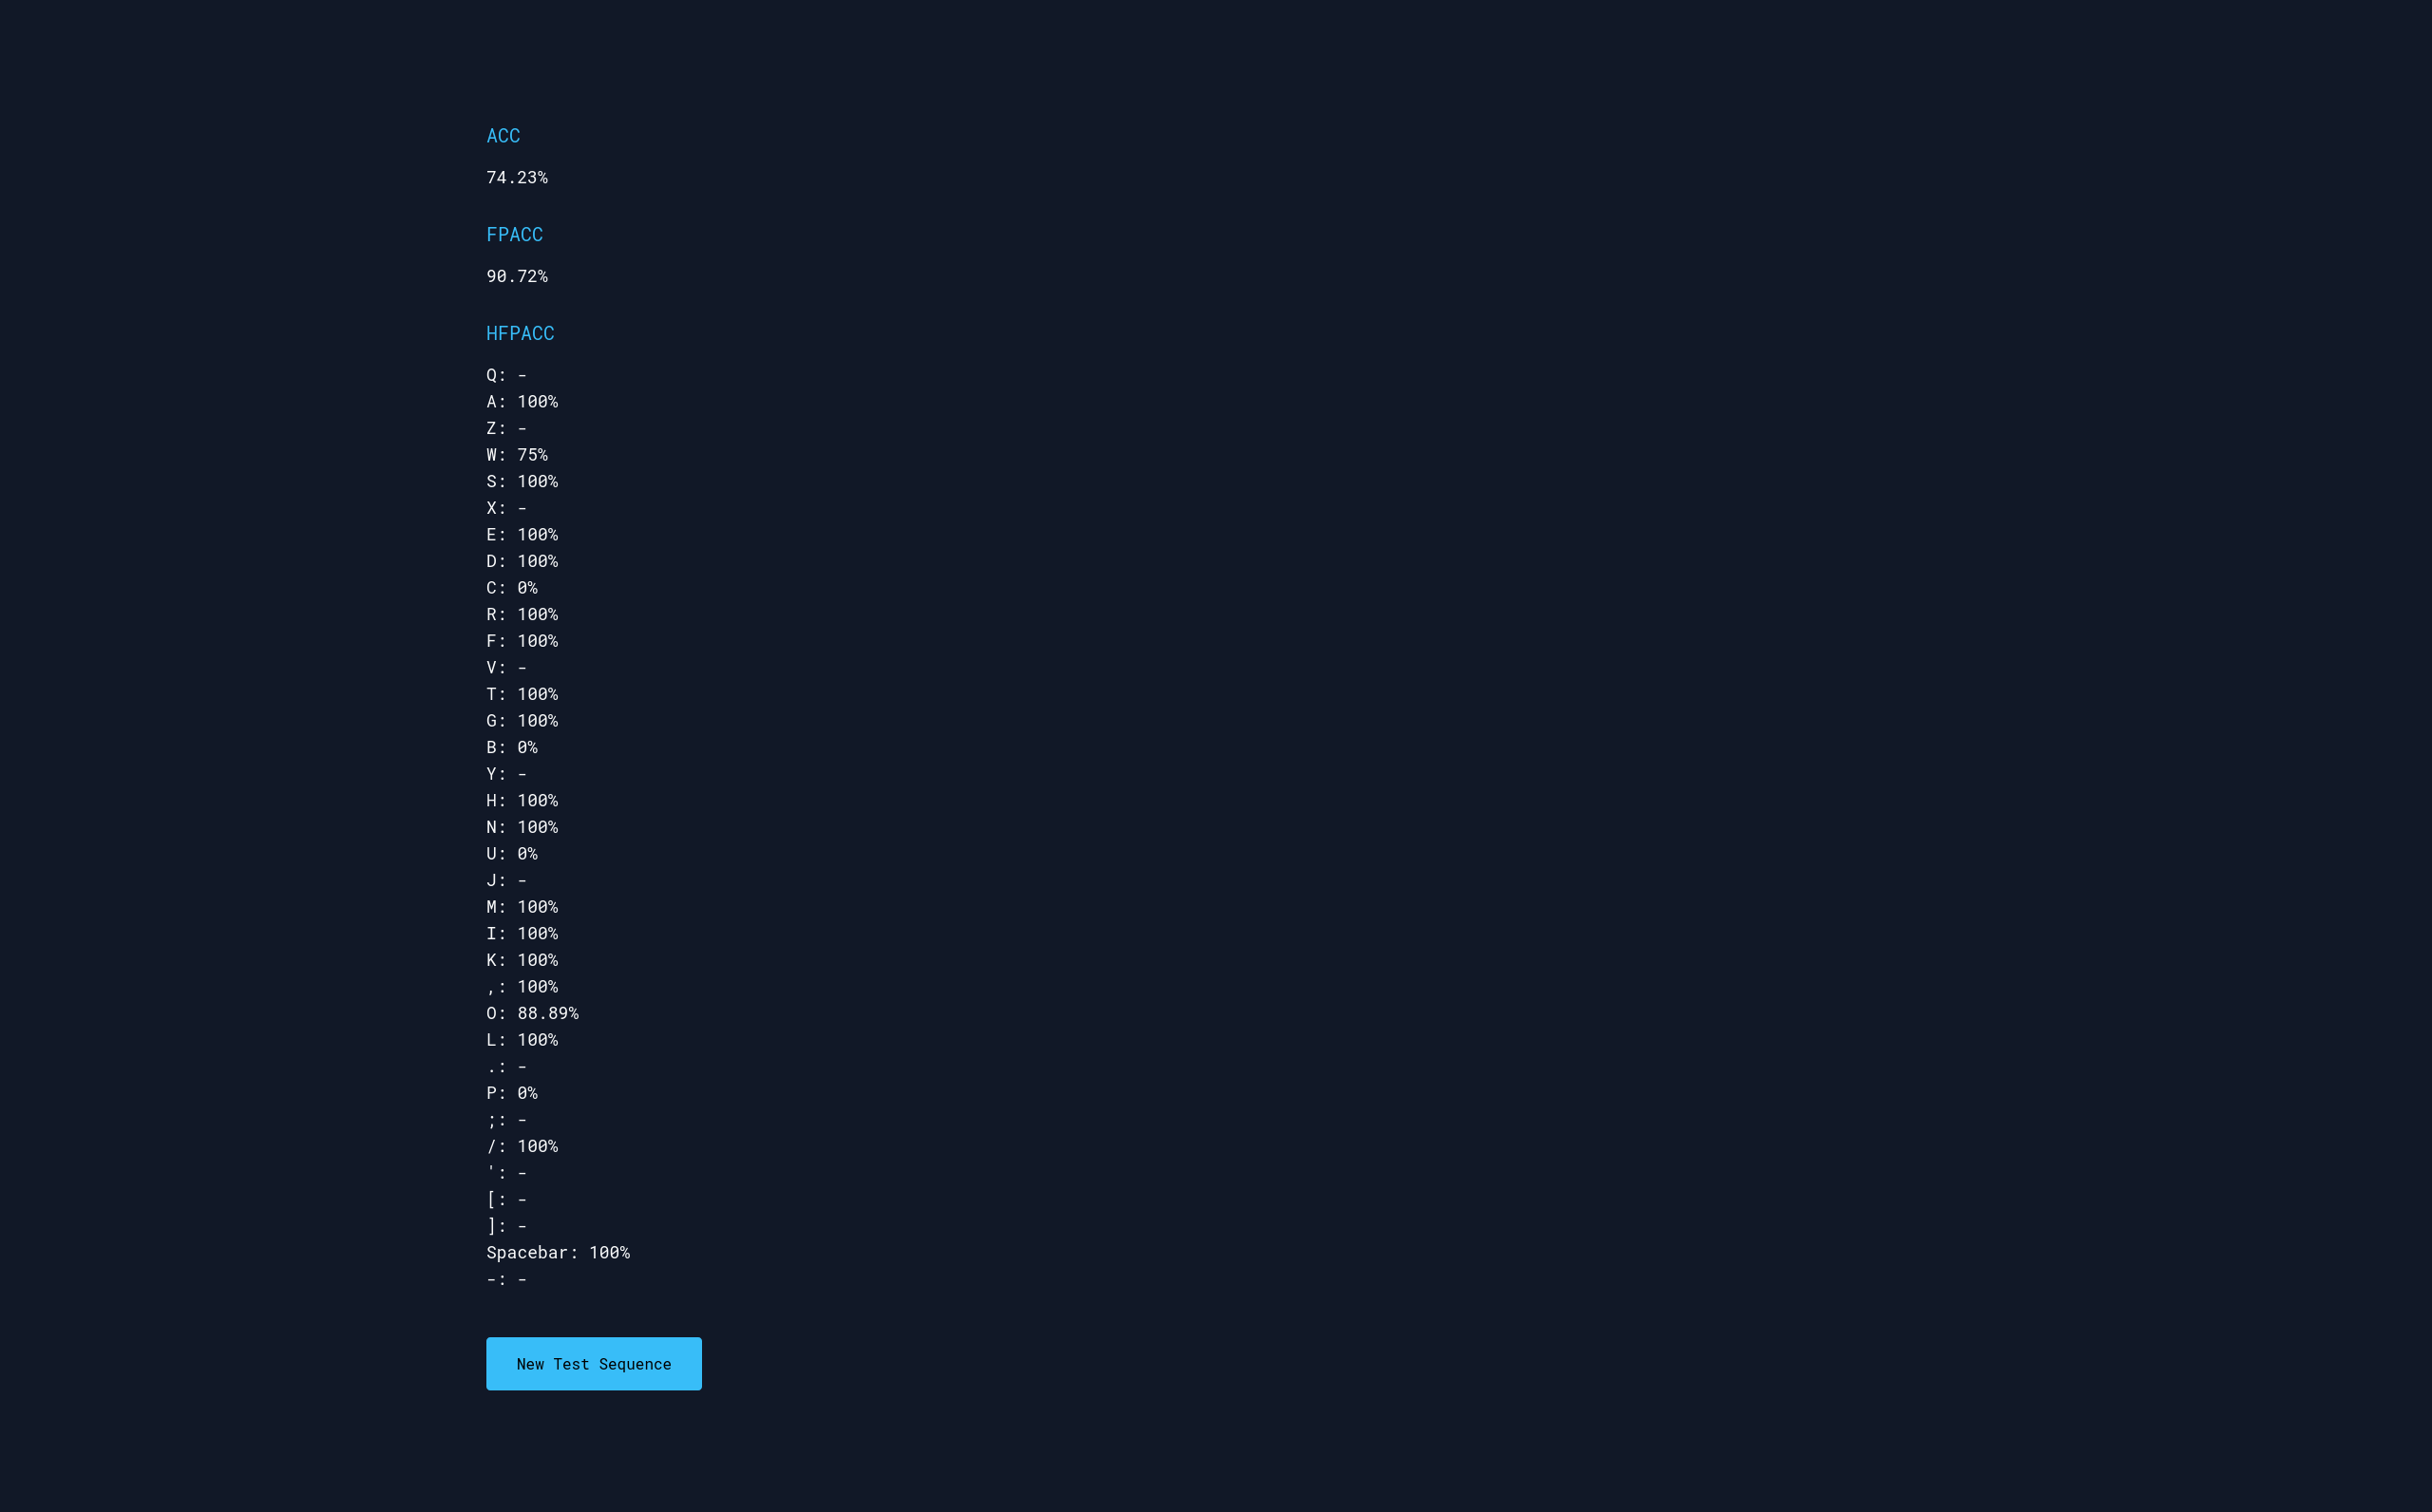
\includegraphics[width=1\textwidth]{frontend-metrics.png}
	\caption{Page presenting the metrics obtained from the trainer}
	\label{fig:metho-front-metrics}
	\centering
\end{figure}

The metrics gathered from the test sequences are shown on a page as illustrated
in Figure~\ref{fig:metho-front-metrics}. This page presents metrics that will be
discussed in Section~\ref{section:metric}. Of note, the metrics shown on this
page that use multiple test sequences as an input uses tests that were obtained
only during the time the page was opened. This proof of concept does not store
the data of a user's previous test sequences that were performed from a
different session.

\subsubsection{Implementation}
The frontend was developed in Svelte, and the backend was developed with Flask.
The frontend handled capturing the video, presenting the layout, and capturing
input events. Finger Tracking was done on the frontend through the use of
MediaPipe Hand's JavaScript library. The frontend also handled checking what
fingertip was inside the \ac{roi} of the key that was entered. The backend
handled the generation of the Key-Edge Coordinates Map using the image passed
from the frontend.

Two of the key steps in the module: finger tracking and integration were
offloaded in the frontend as the wall of latency that exists between the
frontend and the backend would cause performance issues. While this issue also
exists in obtaining the Key-Edge Coordinates Map, this wouldn't affect real-time
finger-key identification since this is a preprocessing step and is not ran
during the time the user performs the typing test.

\section{Metrics}
\label{section:metric}

There were two total metrics obtained pertaining to finger and key mapping. The
first was per test sequence, and the second was per key.

\subsection{Per Test Sequence}
The metric which calculates per test sequence is \ac{fpacc}. This metric
computes the percentage of accurate keys pressed with the correct finger over
the length of the typing test sequence. Inputting the wrong character, even if
pressed with the correct finger, reduces \ac{fpacc} since \ac{fpacc} measures
\emph{accurate key presses}, and incorrect characters are considered inaccurate
key presses.

The equation for calculating \ac{fpacc} is as follows:

\begin{equation}
	FP ACC = \frac{|F|}{|T|} \cdot 100\%
\end{equation}
\labelequations{Finger Placement Accuracy}


Where $|F|$ refers to the number of accurate keys pressed with the
correct finger and $|T|$ refers to the length of the text.

\subsection{Per Key}
This metric, \ac{hfpacc}, computes the accuracy of the user in pressing a
certain key with the correct finger over all test sequences. The same criteria
in determining accurate key presses. This allows the user to easily verify which
keys need attention and training if there is a high frequency of error.

The equation for calculating a key's \ac{hfpacc} is as follows:

\begin{equation}
	HFP ACC_{char} = \frac{|F_{char}|}{|C_{char}|} \cdot 100\%
\end{equation}
\labelequations{Historical Finger Placement Accuracy}

Where $|F_{char}|$ refers to the number of accurate keys pressed with the
correct finger for a certain character, identified as $char$. $|C_{char}|$
refers to the number of times the character has appeared in all test sequences
for the user.

\chapter{Results and Discussion}
\label{section:rd}

\section{Accuracy}
Accuracy, in the context of the finger-key identification module, calculates the
percentage of successful finger-key identifications that the module has
performed. In this case, success is defined as having the expected finger, based
on the manual labeling, equal to the return value of the module. Accuracy is
calculated as:

\begin{equation}
	ACC = \frac{|S|}{|T|}
\end{equation}
\labelequations{Finger-Key Identification Module Accuracy}

Where $|S|$ is the number of successful finger-key identifications, and $|T|$ is
the total number of keypresses for all typing test sequences. This is also
referred to as the success percentage.

\subsection{Training Results}
There were a total of seven training iterations. These training iterations
served as a way to improve the performance of the module by adjusting its
parameters.

\subsubsection{Identifications}

\begin{figure}[H]
	\centering
	\begin{tikzpicture}
		\begin{axis}[
				ybar stacked,
				bar width=30pt,
				xlabel={Training Iteration},
				ylabel={Percentage over total keypresses},
				xmin=1, xmax=7,
				ymin=86, ymax=100,
				xtick={1,2,3,4,5,6,7},
				ytick={86, 86, 88, 90, 92, 94, 96, 98, 100},
				enlargelimits=0.15,
				area legend,
				tick label style={font=\footnotesize},
				legend style={font=\footnotesize},
				label style={font=\footnotesize},
				every axis legend/.append style={cells={anchor=west}},
				ymajorgrids=true,
			]

			\addplot[
				CornflowerBlue,
				fill=CornflowerBlue,
			]
			coordinates {
					(1, 88.54) (2, 89.02) (3, 98.58) (4, 99.62) (5, 98.54) (6, 99.24) (7, 99.55)
				};
			\addplot[
				Salmon,
				fill=Salmon,
			]
			coordinates {
					(1, 11.46) (2, 10.98) (3, 1.42) (4, 0.38) (5, 1.46) (6, 0.76) (7, 0.45)
				};
			\legend{Successes, Failures}


		\end{axis}
	\end{tikzpicture}
	\caption{Identification results of the training iterations}
	\label{fig:rd-training-identification}
\end{figure}

Over the seven training iterations, there was an increase in success percentage
as shown in Figure~\ref{fig:rd-training-identification}. Consequently, there was
also a decrease in failure percentage. There was a total of 1475 total
keypresses for iterations one to three, and 1571 total keypresses for iterations
four to seven.

The increase in total keypresses starting from iteration four was due to adding
multiple tries to the training routine in obtaining the Key-Edge Coordinates
Map. Iterations one through three only tried frame 10 as the source frame for
the module while iterations four through seven tried frames 10, 15, and 20.

There was a need to try different frames since the camera was not consistent in
its ability to focus on the keyboard for each video. In some videos video, the
camera was not focused on the keyboard in frame 10, but it was able to focus on
frame 15. As a result, the total number of available keypresses to test
increased.

The 0.48\% jump between iterations one and two can be attributed to correcting
erroneous finger-key identifications that were obtained from manual labeling.
The 9.56\% jump in success percentage between iterations two and three was due
to adding buffers around the \ac{roi} by scaling the contours by 10 pixels on
each side. Iteration four's increase was due to fixing the image map. Certain
keys had incorrect color values assigned in the Key-Color Values Map, and some
keys were of incorrect shape. Iterations five to seven were performed to test
different values and shapes for scaling the \ac{roi}.

\subsubsection{Uncertain Successes}

\begin{figure}[H]
	\centering
	\begin{tikzpicture}
		\begin{axis}[
				ybar stacked,
				bar width=30pt,
				xlabel={Training Iteration},
				ylabel={Percentage over total keypresses},
				xmin=1, xmax=7,
				ymin=0, ymax=30,
				xtick={1,2,3,4,5,6,7},
				ytick={0,5,10,15,20,25,30},
				enlargelimits=0.15,
				area legend,
				tick label style={font=\footnotesize},
				legend style={font=\footnotesize},
				label style={font=\footnotesize},
				every axis legend/.append style={cells={anchor=west}},
				ymajorgrids=true,
			]

			\addplot[
				CornflowerBlue,
				fill=CornflowerBlue
			]
			coordinates {
					(1, 5.69) (2, 5.69) (3, 12.61) (4, 12.86) (5, 9.32) (6, 10.76) (7, 12.86)
				};
			\addplot[
				Salmon,
				fill=Salmon,
			]
			coordinates {
					(1, 0.61) (2, 0.61) (3, 17.15) (4, 17.06) (5, 3.95) (6, 6.49) (7, 9.68)
				};
			\legend{Spacebar, Non-spacebar}


		\end{axis}
	\end{tikzpicture}
	\caption{Uncertain Successes of the training iterations}
	\label{fig:rd-training-uncertain-successes}
\end{figure}

Uncertain Successes are instances where the finger-key identification module was
able to detect two or more fingertips within the \ac{roi} of the key. As such,
the module is uncertain which of the multiple fingertips pressed the key.
However, it is still classified as a success since the expected finger from the
manual labeling exists within the array of fingertips returned by the module.
Figure~\ref{fig:rd-training-uncertain-successes} shows the trend of this metric
throughout the different training iterations.

\paragraph{Spacebar}
In a 60\% keyboard, the spacebar is the longest key on the keyboard. In
addition, this key is right below the non-dominant hand's thumb default resting
position when the hand's posture follows the proper touch typing posture. As
such, it was to be expected that a majority of the uncertain successes were
because of the spacebar. However, this was not the case for iterations three and
four. This was because the buffer for the \ac{roi} was too big and this caused
the module to detect more than one fingertip within that \ac{roi}.

\paragraph{Non-spacebar}
There were cases where the module had uncertain successes that were not over the
spacebar. In almost practically all cases, these were over the alphanumeric
keys. These uncertain successes stem from the increased buffer of the \ac{roi}.
This type of uncertain success carries more weight compared to spacebar
uncertain successes since the keys where these uncertain successes come from are
the smallest keys on the keyboard. This means that the chances that a person has
two or more fingers over the keys are rare, compared to the spacebar.


\subsubsection{Uncertain Successes vs Success Percentage}
\label{section:rd-uncertain vs success}

\begin{figure}[H]
	\centering
	\begin{tikzpicture}
		\begin{axis}[
				xlabel={Training Iteration},
				ylabel={Percentage over total keypresses},
				xmin=1, xmax=7,
				ymin=0, ymax=100,
				xtick={1,2,3,4,5,6,7},
				ytick={0,20,40,60,80,100},
				tick label style={font=\footnotesize},
				legend style={font=\footnotesize},
				label style={font=\footnotesize},
				enlargelimits=0.15,
				ymajorgrids=true,
				xmajorgrids=true,
				nodes near coords,
				every node near coord/.append style={font=\footnotesize},
				every axis legend/.append style={at={(0.98, 0.02)}, anchor=south east, cells={anchor=west}}
			]

			\addplot[
				color=CornflowerBlue,
				mark=square,
			]
			coordinates {
					(1, 88.54) (2, 89.02) (3, 99.58) (4, 99.62) (5, 98.54) (6, 99.24) (7, 99.55)
				};
			\addplot[
				color=Salmon,
				mark=square,
			]
			coordinates {
					(1, 6.31) (2, 6.31) (3, 29.76) (4, 29.92) (5, 13.18) (6, 17.25) (7, 22.53)
				};

			\legend{Successes, Total Uncertain Successes}

		\end{axis}
	\end{tikzpicture}
	\caption{Uncertain Successes of the training iterations}
	\label{fig:rd-training-uncertain-successes-vs-success}
\end{figure}


Tuning the algorithm required managing both uncertain successes and the success
percentage and making compromises between one or the other. The goal of the
training process was to maximize the success percentage while limiting the
number of uncertain successes.

As seen in Figure~\ref{fig:rd-training-uncertain-successes-vs-success}, it can
be noted that in iterations one and two, the success rate was lower compared to
the other iterations. However, the percentage of uncertain successes was also
the lowest. Iteration three was the first iteration that created a buffer around
each key, however, this buffer of 10 pixels was too aggressive, with the
uncertain successes spiking upwards to nearly 30\%. Iteration five reduced the
buffer size by half to five pixels. This did not affect the success rate that
much, with only a reduction of 1.08\%. This also greatly decreased the uncertain
success percentage by 16.74\%. The sixth iteration met halfway between
iterations four and five, by adding a buffer of seven pixels. This increased the
success rate back to 99.24\% without greatly increasing the number of uncertain
successes. In comparison with the fourth iteration, the sixth iteration had its
success rate decrease by 0.38\%, but its percentage of uncertain successes
decreased by 12.67\%. A seventh iteration was trialed where the increase in
buffer was asymmetrical. For each key, the points nearer the user were increased
by 10 pixels, while the points farther away were increased by five pixels only.
This slightly increased the success rate by 0.31\%. However, the percentage of
uncertain successes also increased by 5.28\%.

While the percentage of uncertain successes in iterations five through seven was
in the range of 13\% to 20\%, The majority of these uncertain successes were
spacebar uncertain successes, as shown in
Figure~\ref{fig:rd-training-uncertain-successes}.

Based on these results, the final selected parameters for the module were the
parameters set in iteration six, with the buffer set to seven pixels as it was a
good middle ground between success rate and uncertain successes.


\subsubsection{Failure Types}

\begin{figure}[H]
	\centering
	\begin{tikzpicture}
		\begin{axis}[
				ybar stacked,
				bar width=30pt,
				xlabel={Training Iteration},
				ylabel={Percentage over total keypresses},
				xmin=1, xmax=7,
				ymin=0, ymax=15,
				xtick={1,2,3,4,5,6,7},
				ytick={0,3,6,9,12,15},
				enlargelimits=0.15,
				area legend,
				tick label style={font=\footnotesize},
				legend style={font=\footnotesize},
				label style={font=\footnotesize},
				every axis legend/.append style={cells={anchor=west}},
				ymajorgrids=true,
			]

			\addplot[
				CornflowerBlue,
				fill=CornflowerBlue
			]
			coordinates {
					(1, 0.47) (2, 0) (3, 0.14) (4, 0) (5, 0) (6, 0) (7, 0)
				};
			\addplot[
				Salmon,
				fill=Salmon,
			]
			coordinates {
					(1, 10.98) (2, 10.98) (3, 1.29) (4, 0.38) (5, 1.46) (6, 0.76) (7, 0.45)
				};
			\legend{Mismatched Detection, No Detection}


		\end{axis}
	\end{tikzpicture}
	\caption{Uncertain Successes of the training iterations}
	\label{fig:rd-training-failure-types}
\end{figure}

\begin{figure}[H]
	\centering
	\begin{subfigure}{.5\textwidth}
		\centering
		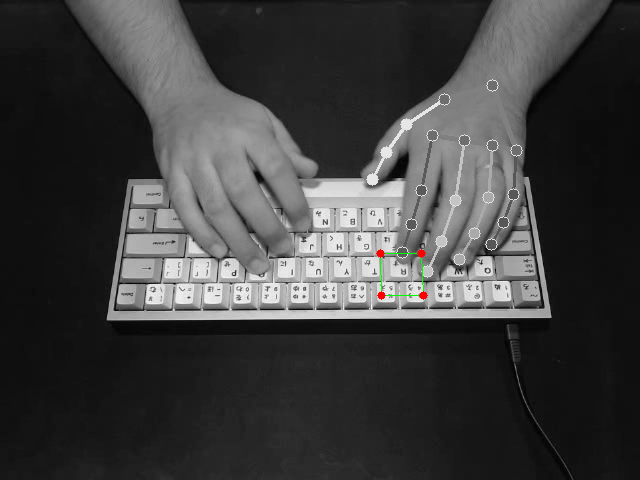
\includegraphics[width=.995\linewidth]{failure-3.png}
	\end{subfigure}\\
	\begin{subfigure}{.5\textwidth}
		\centering
		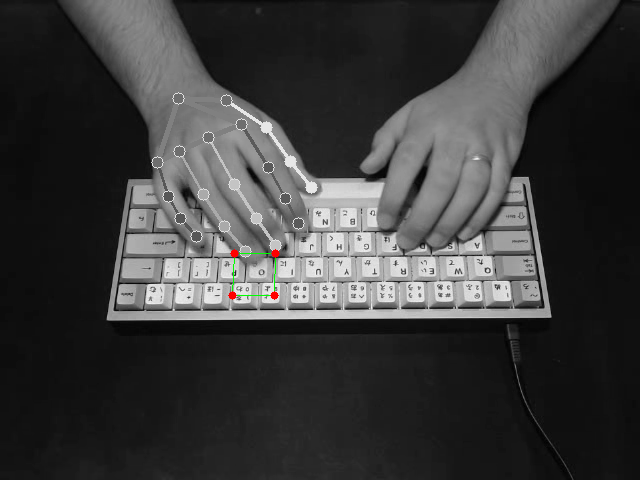
\includegraphics[width=.995\linewidth]{failure-1.png}
	\end{subfigure}%
	\begin{subfigure}{.5\textwidth}
		\centering
		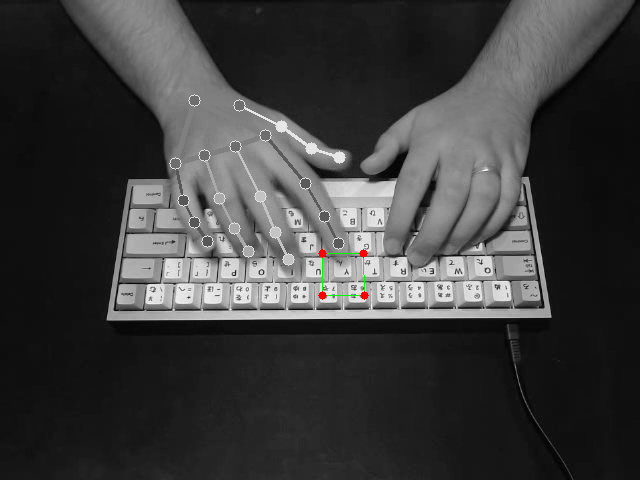
\includegraphics[width=.995\linewidth]{failure-2.png}
	\end{subfigure}
	\caption{Example of No Identification Failures}
	\label{fig:rd-training-sample}
\end{figure}

\paragraph{Mismatched Identification}
These are failures where the module did not return the expected fingertip based
on the manual labeling. This type of failure only manifested in iterations one
and three. The failures in iteration one, after double-checking the video, were
due to an error during manual labeling. In iteration three, these errors were
due to an incorrect image map and Key-Color Values map. The information for some
keys was not consistent between both.

Based on this information and from the gathered data as shown in
Figure~\ref{fig:rd-training-failure-types}, this failure type is non-existent
for the module in real-life conditions.

\paragraph{No Identification}
These are failures where the module did not detect any fingertips within the
\ac{roi}. Figure~\ref{fig:rd-training-sample} shows examples of frames where
these errors occurred. These made up all the failures from the test results.
These types of failures occurred because the fingertips used to press the key
were not directly above the key, but rather offset to its side. Scaling the
\ac{roi} would reduce the number of no identification failures, but it would
also increase the number of uncertain successes. See
Section~\ref{section:rd-uncertain vs success}, Uncertain Successes vs Success
Percentage for more information.

\subsubsection{Occlusion}
The module was also successful in finger-key identification, even if both the
key and finger were occluded. Figure~\ref{fig:rd-occluded} is one frame where
this occurred. The module was successful in identifying that the Left Thumb was
used to press the Left Shift.

\begin{figure}[H]
	\centering
	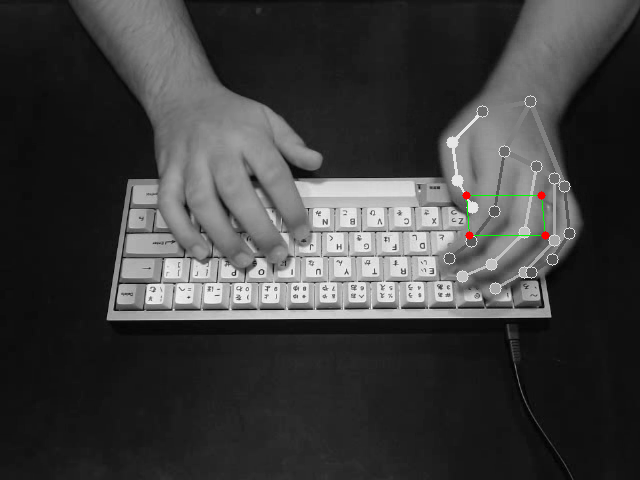
\includegraphics[width=0.8\textwidth]{occluded.png}
	\caption{Occluded finger and key}
	\label{fig:rd-occluded}
\end{figure}


\subsection{Test Results}
\begin{table}[H]
	\small
	\centering
	\caption{\label{tab:rd-accuracy}Accuracy Results of the Module with Test Data}
	\begin{tabular}{ p{0.4\textwidth} R{0.2\textwidth} }
		\toprule
		Category                        & Value   \\
		\midrule
		Total Keypresses                & 942     \\[0.25cm]
		\midrule
		Identifications                           \\
		\midrule
		Successes                       & 938     \\
		Failures                        & 4       \\
		Success Percentage / Accuracy   & 99.58\% \\
		Failure Percentage              & 0.42\%  \\[0.25cm]
		\midrule
		Failure Types                             \\
		\midrule
		Mismatched Identification       & 0       \\
		No Identification               & 4       \\[0.25cm]
		\midrule
		Uncertain Successes                       \\
		\midrule
		Total                           & 133     \\
		Spacebar                        & 72      \\
		Spacebar Percentage             & 54.14\% \\
		Spacebar Percentage (Total)     & 7.64\%  \\
		Non-spacebar                    & 61      \\
		Non-spacebar Percentage         & 45.86\% \\
		Non-spacebar Percentage (Total) & 6.48\%  \\
		\bottomrule
	\end{tabular}
\end{table}

Table~\ref{tab:rd-accuracy} provides the accuracy results of the module with
test data. These results were satisfactory after running the module with the
parameters from the sixth training iteration on the test data. There was another
run with the same test data and the same parameters, however, these results were
omitted since this run had inconclusive results as there was a single
identification that was incorrectly labeled during manual finger-key
identification.

\section{Speed}

Based on the definition of \ac{wpm} from \textcite{arif2009} as seen in
Equation~\ref{equ:wpm}, it can be extrapolated that calculating \ac{cps} is:

\begin{equation}
	CPS = \frac{WPM}{60} \cdot 5
	\label{eq:cps}
\end{equation}
\labelequations{Characters per Second}

The average \ac{wpm} when typing using the QWERTY layout, according to test data
from \citeauthor{keybr} is $\approx37.5$ \ac{wpm}. As such, we can calculate
that the average Characters per Second when typing using the QWERTY layout is
3.125. We can calculate the seconds needed per character by this equation:

\begin{equation}
	s = \frac{1}{CPS}
	\label{eq:s}
\end{equation}
\labelequations{Seconds per Character}

This means that each character, on average, requires 0.32 seconds to type. This
sets the maximum time spent for finger-key identification for a single
character. Any more than this would result in a noticeable slowdown during
typing.

\subsection{Results}

\subsubsection{Training Iterations}

\begin{figure}[H]
	\centering
	\begin{tikzpicture}
		\begin{axis}[
				xlabel={Training Iteration},
				ylabel={Seconds},
				xmin=1, xmax=7,
				ymin=0, ymax=1,
				xtick={1,2,3,4,5,6,7},
				ytick={0, 0.1, 0.2, 0.3, 0.4, 0.5, 0.6, 0.7, 0.8, 0.9, 1.0},
				tick label style={font=\footnotesize},
				legend style={font=\footnotesize},
				label style={font=\footnotesize},
				enlargelimits=0.15,
				ymajorgrids=true,
				xmajorgrids=true,
				nodes near coords,
				every node near coord/.append style={font=\footnotesize},
				every axis legend/.append style={cells={anchor=west}}
			]

			\addplot[
				color=CornflowerBlue,
				mark=square,
			]
			coordinates {
					(1, 0.9123) (2, 0.8225) (3, 0.8144) (4, 0.8211) (5, 0.8258) (6, 0.8366) (7, 0.8118)
				};
			\addplot[
				color=Salmon,
				mark=square,
			]
			coordinates {
					(1, 0.0895) (2, 0.0903) (3, 0.0823) (4, 0.0835) (5, 0.0845) (6, 0.0828) (7, 0.0797)

				};
			\legend{Avg. Keyboard Detection Time, Avg. Finger Identification Time}

		\end{axis}
	\end{tikzpicture}
	\caption{Keyboard detection time of the training iterations}
	\label{fig:rd-training-keyboard-detection-time}
\end{figure}

The training iterations had an average keyboard detection time of
$0.8620\pm0.0502s$ and average finger identification time of $0.0863\pm0.0040s$.
Throughout the training, there was no noticeable difference in running time over
the same dataset as shown in
Figure~\ref{fig:rd-training-keyboard-detection-time}. However, the first
training iteration had issues with gathering the speed of the module, as the
average keyboard detection time included other operations that were not part of
getting the Key-Edge Coordinates Map. Removing this iteration, the average
keyboard detection time becomes more consistent, with it being
$0.8295\pm0.0070s$.

\subsubsection{Test Results}

\begin{table}[H]
	\small
	\centering
	\caption{\label{tab:rd-speed}Speed Results of the Module with Test Data}
	\begin{tabular}{ p{0.4\textwidth} R{0.2\textwidth} }
		\toprule
		Category                        & Seconds \\
		\midrule
		Avg. Keyboard Detection Time    & 0.838   \\
		Avg. Finger Identification Time & 0.083   \\
		\bottomrule
	\end{tabular}
\end{table}

These results, as tabulated in Table~\ref{tab:rd-speed} were consistent with the
training iterations. This means that the module has repeatable and predictable
running times.

\subsection{Average Keyboard Detection Time}
This is the time that was measured as the module generated the Key-Edge
Coordinates Map. This corresponds with the first step of the module. It is to be
noted that this time does not affect keyboard typing and is not limited by the
0.32 threshold as the user is not yet typing at this point.

\subsection{Average Finger Identification Time}
This is the time spent in finger-key identification for a single key. As such,
this time should be below 0.32 seconds for the module to be capable of
performing finger-key identification in real-time without noticeable slowdown
from the perspective of the user.

The average finger identification time that the module got was 0.083s which is
well below 0.32s. This can be attributed to the speed of the MediaPipe library,
and the pre-calculation of the edge coordinates.

\subsubsection{Real-Time Finger-Key Identification}
With each keypress only requiring 0.083s for finger-key identification, it can
be gathered that the maximum \ac{cps} which the module can still perform
real-time finger-key identification is 11.9200 \ac{cps}, based on
Equation~\ref{eq:s}. It follows that the maximum \ac{wpm} that still allows for
real-time finger-key identification is 143.040 \ac{wpm}, based on
Equation~\ref{eq:cps}. This is well above the median of 37.5 \ac{wpm} on Keybr.
The module can also perform real-time finger-key identification for 90.99\% of
the community members of Monkeytype with the speed role.

\chapter{Conclusion}

The finger key identification module was successfully developed and implemented
in this study.

The finger-key identification solution was split into two parts, keyboard
detection and key mapping, and finger detection. Keyboard detection and key
mapping used the following algorithm and techniques: (1) Edge Detection using
Sobel filter \parencite{sobel2014}, (2) Thresholding using Otsu's algorithm
\parencite{otsu}, (3) Finding contours using the algorithm of
\textcite{contours}, (4) Line Simplification using the Douglas-Peucker algorithm
\parencite{douglas-peucker}, and (5) Perspective transform
\parencite{opencv-image-transform}. Finger detection utilized a ready-made
solution called MediaPipe Hands by \textcite{mediapipe}. The two were combined
to perform finger-key identification.

The keyboard used was a 60\% keyboard in ANSI. It was light in color and was
connected with a black USB-C cable. The surface of the desk was dark, and a LED
Bulb rated at 9 Watts, 700 lumens, and 6500k color temperature was used to
uniformly light the capture area. The single optical camera, a Logitech C920,
was placed above the keyboard, pointing directly downwards. It captured videos
in 720p/30fps with a diagonal field of view of 78\degree \parencite{logitech}.
The computer used had an AMD Ryzen 5 3600 CPU, AMD Radeon RX 5600 XT GPU,
G.Skill Trident Z Neo RGB 16GB 3200mhz RAM, and Samsung SSD 850 EVO SSD.

The development of the module utilized OpenCV as the main image manipulation
platform that implemented the algorithms mentioned previously. OpenCV was also
used to capture videos from the optical camera. It was all written in Python.

The module was accurate in 99.58\% of identifications in a data set composed of
942 keypresses. However, 14.12\% of the identifications were uncertain
successes. These are successes where more than one fingertip was found in an
\ac{roi}. Of these, 6.48\% were non-spacebar uncertain successes. These are
uncertain successes over keys that are not the spacebar. This bears more weight
since most of these keys are the smallest on the keyboard, and in most cases,
only one fingertip could fit within the key. These uncertain successes were due
to the addition of a buffer around each \ac{roi} to increase the success rate.

The module is fast enough for real-time finger-key identification up to typing
speeds of 143.040 \ac{wpm}. This is above the median typing speed of 37.5
\ac{wpm} on Keybr \parencite{keybr}. This also handles 90.99\% of the 12678
members with the speed role on Monkeytype \parencite{monkey-stats}.

Two metrics were developed and implemented in a proof of concept trainer: (1)
Finger Placement Accuracy which computes the percentage of keys pressed with the
correct figure over the length of the test sequence, and (2) Historical Finger
Placement Accuracy which computes the number of times the user is successful if
pressing a key with the correct finger over all test sequences.

\chapter{Future Work}


\section{Trainer}
A proof of concept trainer with real-time finger-key identification was
developed, however this trainer is lacking in functionality to be an actual
usable trainer that will be used for educational purposes.

In addition, the wall of latency that exists during th Key-Edge Coordinates Map
can be removed by doing this process on the browser. This can be done by redoing
the process in C, and compiling that to WebAssembly. The MediaPipe team did the
same thing for MediaPipe Hands, and performance, for this use case, was more or
less equal.

\section{Standardized Finger-Key Mapping}
While there are mappings for the default ANSI and ISO layouts, these layouts
were not official and were defacto standards. While the trainer uses this
defacto standard, it wouldn't be difficult to adapt the trainer to use another
standard for finger-key mapping.


\section{Character Representation}
The test and training data did not have equal representation of the keys within
the keyboard. For the module to undergo more rigorous testing, it would be
better to have a dataset that has equal representation of all of the characters
in the keyboard.

\section{Effects on Touch Typing Education}
The paper created a method for finger-key identification in hopes of improving
touch typing education, however, there was no test done to prove that the module
will affect the learner's skill in touch typing

\section{Effects on Health}
In connection with the previous section, the module also has no testing done to
quantify if training using the module will improve the posture and reduce
problematic hand positions and movements that can cause nerve and muscular
disorders.

\section{Environmental Setup}
The environmental setup was tightly controlled, with the keyboard and the desk
of contrasting color, lighting was nearly perfect, and the camera was of great
quality. This is not realistic and is not representative of the real world.
Future work could improve upon this area. An idea would be to have a separate
process where the user could just select four points rather than relying on an
automated computer vision process to detect the four edges.

\section{ROI Buffer}
The buffer was selected after trail and error in the training phase of the
algorithm. However, this buffer may not be the best and adaptive techniques or a
machine learning algorithm may select better values for the buffer.

\section{Detecting Keyboard Movement Between Frames}
The module is limited in its ability to track keyboards that move between
keypresses. While this is not something that usually happens during keyboard
typing, having the ability to track movements would be a great addition to
improving the module's performance.

\section{Different Keyboard Types, Layouts, and Colors}
The module is limited to detecting keypresses with a 60\% keyboard. This type of
keyboard is not that commonly used. Other keyboard types, like the 100\%, 75\%,
and TKLs would be good starting points for adding support. In addition,
supporting other layouts, like ISO, would also greatly increase the number of
people that could use the module. Furthermore, supporting other color schemes
would also widen the number of keyboards that can be used with the module.

\newpage
\appendix

\twocolumn
\chapter{Key-Color Values Map}
\label{appendix:key-map}

\tablehead{\toprule Key &\multicolumn{1}{l}{Color (in BGR)} \\ \midrule}
\tabletail{%
	\midrule \multicolumn{2}{r}{{Continued on next column}} \\ \midrule}
\tablelasttail{%
	\\\midrule
	\multicolumn{2}{r}{{Concluded}} \\ \bottomrule}
\centering
\small
\begin{supertabular}{ll}
	LeftControl & (85, 0, 0)\\
	LeftSuper & (45, 0, 0)\\
	LeftAlt & (58, 35, 0)\\
	Spacebar & (62, 55, 0)\\
	RightAlt & (0, 28, 44)\\
	RightSuper & (0, 3, 73)\\
	RightControl & (24, 0, 76)\\
	` & (255, 0, 0)\\
	1 & (255, 153, 0)\\
	2 & (255, 229, 0)\\
	3 & (189, 255, 0)\\
	4 & (143, 255, 0)\\
	5 & (51, 255, 0)\\
	6 & (0, 255, 102)\\
	7 & (0, 255, 194)\\
	8 & (0, 224, 255)\\
	9 & (0, 163, 255)\\
	0 & (0, 102, 255)\\
	- & (0, 10, 255)\\
	= & (82, 0, 255)\\
	$\vert$ & (128, 0, 255)\\
	Delete & (189, 0, 255)\\
	Tab & (224, 0, 0)\\
	Q & (214, 128, 0)\\
	W & (225, 203, 0)\\
	E & (160, 217, 0)\\
	R & (126, 224, 0)\\
	T & (43, 217, 0)\\
	Y & (0, 216, 86)\\
	U & (0, 195, 149)\\
	I & (0, 183, 208)\\
	O & (0, 136, 212)\\
	P & (0, 79, 196)\\
	] & (0, 8, 211)\\
	{[} & (63, 0, 196)\\
	Backspace & (134, 0, 181)\\
	CapsLock & (195, 0, 0)\\
	A & (167, 100, 0)\\
	S & (178, 161, 0)\\
	D & (124, 168, 0)\\
	F & (101, 180, 0)\\
	G & (31, 157, 0)\\
	H & (0, 139, 56)\\
	J & (1, 139, 106)\\
	K & (0, 130, 148)\\
	L & (0, 94, 147)\\
	; & (0, 52, 130)\\
	' & (0, 7, 170)\\
	Enter & (35, 0, 109)\\
	LeftShift & (150, 0, 0)\\
	Z & (104, 62, 0)\\
	X & (130, 117, 0)\\
	C & (77, 104, 0)\\
	V & (63, 113, 0)\\
	B & (18, 88, 0)\\
	N & (0, 66, 26)\\
	M & (0, 84, 64)\\
	, & (0, 75, 85)\\
	. & (0, 70, 109)\\
	/ & (0, 32, 80)\\
	RightShift & (0, 5, 128)\\

\end{supertabular}

\onecolumn
\chapter{Typing Test Sequences}
\label{appendix:test-sequences}
\normalsize
\begin{enumerate}
	\item ``What of it, if some old hunks of a sea-captain orders me to get a broom and sweep down the decks?'' \parencite{moby-dick}
	\item ``I sat down on an old wooden settle, carved all over like a bench on the Battery.'' \parencite{moby-dick}
	\item ``I lay there dismally calculating that sixteen entire hours must elapse before I could hope for a resurrection.'' \parencite{moby-dick}
	\item ``How slowly the time passes here, encompassed as I am by frost and snow!'' \parencite{frankenstein}
	\item ``I listened to my father in silence and remained for some time incapable of offering any reply.'' \parencite{frankenstein}
	\item ``Think you’re escaping and run into yourself. Longest way round is the shortest way home.'' \parencite{ulysses}
	\item ``History, Stephen said, is a nightmare from which I am trying to awake'' \parencite{ulysses}
	\item ``A man of genius makes no mistakes. His errors are volitional and are the portals of discovery.'' \parencite{ulysses}
	\item ``Never trust to general impressions, my boy, but concentrate yourself upon details'' \parencite{sherlock}
	\item ``I have no data yet. It is a capital mistake to theorise before one has data.'' \parencite{sherlock}
\end{enumerate}

\chapter{Screenshots of Data Analysis}
\label{appendix:sheets}

\begin{figure}[H]
	\centering
	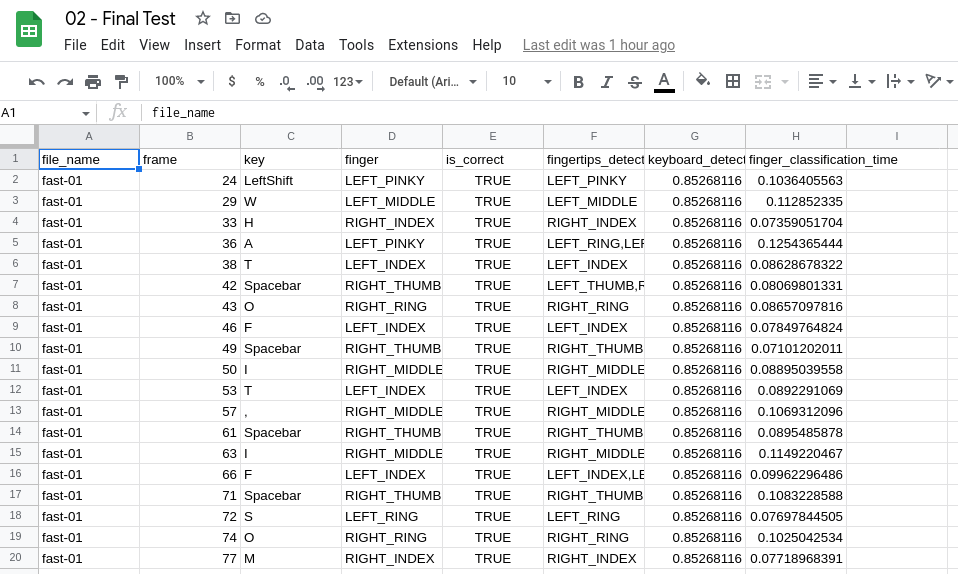
\includegraphics[width=0.8\textwidth]{sheets-raw-data.png}
	\caption{Raw data as seen on Google Sheets}
\end{figure}

\begin{figure}[H]
	\centering
	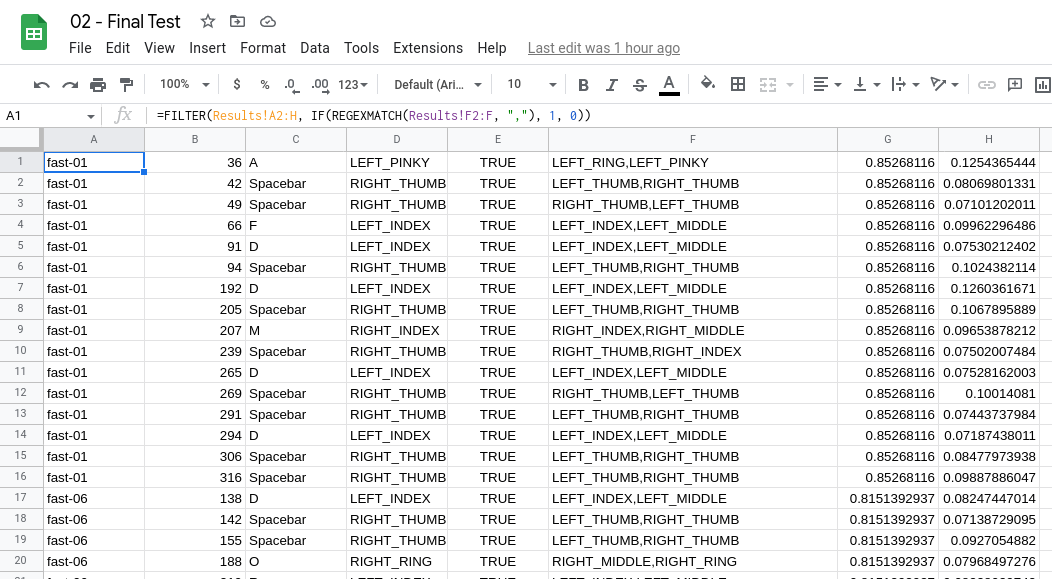
\includegraphics[width=0.8\textwidth]{sheets-uncertain.png}
	\caption{Filtered raw data to show uncertain successes}
\end{figure}

\begin{figure}[H]
	\centering
	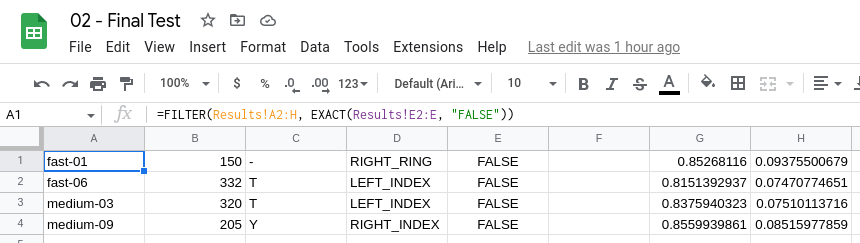
\includegraphics[width=0.8\textwidth]{sheets-failures.png}
	\caption{Filtered raw data to show failures}
\end{figure}

\begin{figure}[H]
	\centering
	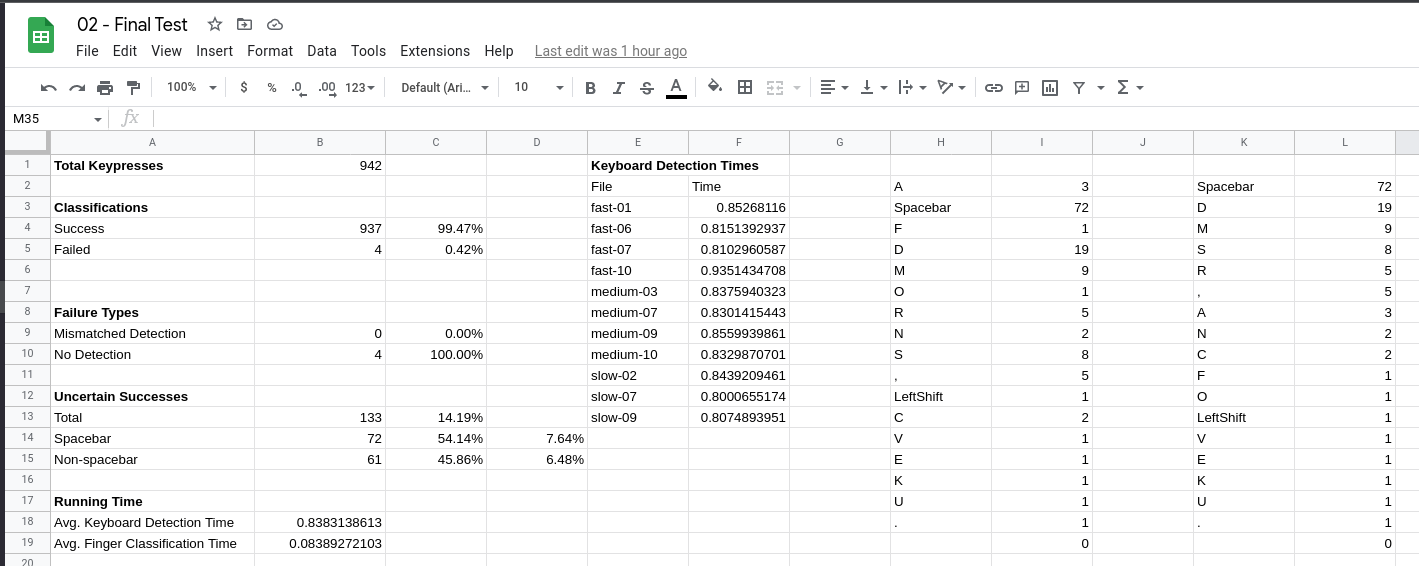
\includegraphics[width=0.8\textwidth]{sheets-analysis.png}
	\caption{Metrics calculated from the raw data}
\end{figure}

\chapter{Gantt Chart}
\begin{landscape}
	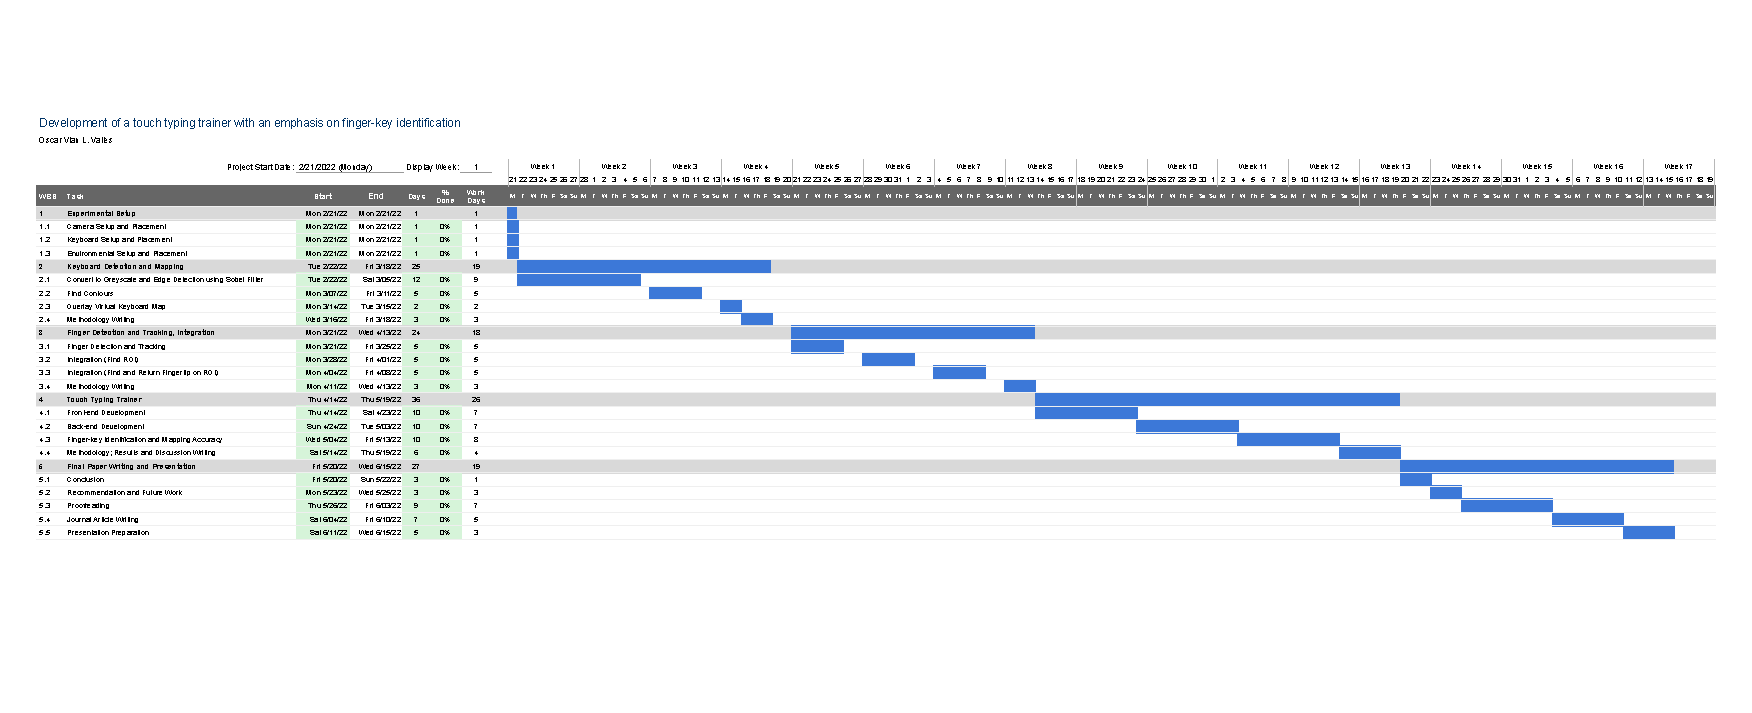
\includepdf[pages=-,landscape,scale=0.8,pagecommand={}]{images/gantt-chart.pdf}
\end{landscape}

\newpage
\printbibliography[heading=bibintoc,title={References}]{}

\end{document}
